% !TeX spellcheck = en_GB
% %%% ***************** CHAPTER RESULTS ***************** %%%
%%%%%%%%% Snowfall comparison model MEPS %%%%%%%%%%%%%%
\section{Snow}
After the analysis of meteorological quantities, the snow at Haukeliseter during the Christmas storm will be investigated.
\\
First the results from the optimal estimation retrieval scheme will be examined and compared to the observations of the double fence. After the overestimation of surface accumulation will be analysed, followed by a vertical comparison of observed estimates of snow water content and predictions. The sections finishes with the relation between wind and precipitation related to the surrounding topography at Haukeliseter. 
%%%%%%%%%%%%%%%%%%%%%%%%%%%%%%%%%%%%%%%%%%%%%%%%%%%%%%%%%%%%%%%%%%%%%%%%%%
\newpage
%%%%%%%%% retrieval sensitivity study %%%%%%%%%%%%%%
\subsection{Sensitivity of the Optimal Estimation Retrieval}\label{sec:ret:sensitivity}
%%%%%%% image observed ice crystals %%%%%%%%%%%%%%%%
\begin{figure}[h]
	\centering
	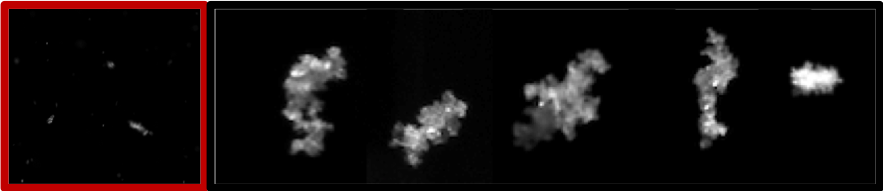
\includegraphics[width=0.8\textwidth]{./MASC_obs/blow_part}
	\caption{MASC particle images of small ground-up blowing snow (red frame) and rimed aggregates (five images to the right). Images taken during the Christmas storm 2016. }\label{fig:ret:all_part}
\end{figure}
%%%%%%%%%%%%%%%%%%%%%%%%%%%%%%%%%%%%%%%%%%%%%%
\noindent
% \textcolor{red}{Include some more specific: Which observations, which quantity was used to generate the optimal estimation retrieval? }
The optimal estimation retrieval scheme for snow was applied to the six-day Christmas 2016 storm event.  MASC images of snow particles during the event were used to guide the selection of the appropriate particle model and PSD input for the retrieval scheme. In this section, the sensitivity of retrieval results to these inputs is explored for the \SI{22}{\dec} as an example. 
This day is used as an example day because it showed the smallest difference between double fence gauge and retrieved surface amount (\Cref{sec:ret_dofe_comp}) during the 2016 Christmas event.
Such an exercise should also allow an identification of those properties that yield the best match with Met-Norway snow gauge measurements at Haukeliseter.  
\\
The majority of the MASC images from Haukeliseter contained snow particles that looked like the left image \Cref{fig:ret:all_part} (red frame). Such images suggest small ground-up blowing snow particles that are consistent with the high winds observed during the event.  However, a careful examination of the MASC images finds the presence of rimed aggregates such as those in the right five images (\Cref{fig:ret:all_part}). Pristine crystals such as plates and columns were not observed during the Christmas 2016 event.  As such, the use of two different aggregate particle models developed for the CloudSat mission are further investigate (\Cref{fig:ret:all_part}). 
\\
\Cref{fig:ret_sensitivity} presents hourly measured surface precipitation amounts on \SI{22}{\dec} plotted against retrieved values for the two different aggregate assumptions. The 'B8' aggregate is a low reflectivity per unit mass aggregate that worked well for the cold, dry conditions observed at Barrow as described in \citet{cooper_variational_2017}. The 'B6' aggregate, presented in \Cref{app:scat_scheme}, is a high reflectivity per unit mass particle (\Cref{sec:ret_scheme}).  As such, the 'B6' aggregate would seem more physically consistent with the observed rimed particles (\Cref{fig:ret:all_part}, 5 aggregates to the right) and humid environment found in the coastal mountains at Haukeliseter.  The presence of a water or rimed coating on the aggregates aloft would greatly enhance their effective reflectivity. 
\\
%\Cref{fig:ret_sensitivity} shows an example of observed and retrieved surface accumulation if the 'B6' or 'B8' particle model is applied on \SI{22}{\dec}.
Indeed, \Cref{fig:ret_sensitivity} suggests that the reflective 'B6' aggregate agree much better than the less reflective 'B8' aggregate with the snow gauge. During the Christmas storm 2016 the assumption of the 'B8' aggregate shows overestimation of precipitation amount at the ground compared to the double fence gauge for all six-days.
%
\\
%%%%%%% image acc B6,B8 %%%%%%%%%%%%%%%%
\begin{figure}[t]
	\centering
	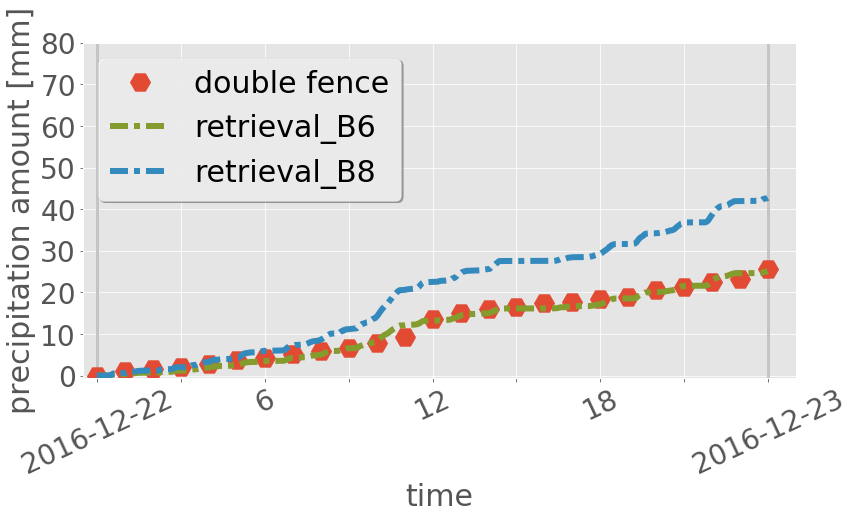
\includegraphics[width=0.75\textwidth]{./fig_obs_ret/20161222_2}
	\caption{Hourly double fence surface precipitation accumulations [mm] plotted against retrieved values for \SI{22}{\dec} for different retrieval assumptions permutations. Double fence precipitation accumulation, red hexagons, retrieved precipitation amount for the here used study (B6), green, dash-dotted, and for small aggregates (B8), blue dashed.}\label{fig:ret_sensitivity}
\end{figure}
%%%%%%%%%%%%%%%%%%%%%%%%%%%%%%%%%%%%%%%%%%%%%%
\\
\Cref{tab:res:ret_sens} presents the percentage differences between snow gauge and retrieved estimates found when using these particle model assumptions for \SI{22}{\dec}. Use of the 'B6' aggregate agreed within \SI{5}{\percent} of the double fence observations (\Cref{tab:res:ret_sens}) for both \SI{12}{\hour} and \SI{24}{\hour} surface accumulations. Admittedly, use of the ‘B6’ aggregate produced slightly too little snow amount relative to the gauges for the remaining days of the event as discussed in \Cref{sec:ret_dofe_comp}. The use of the ‘B8’ aggregate, however, overestimates accumulated snow by at least \SI{65}{\percent} for both the \SI{12}{\hour} and \SI{24}{\hour} surface accumulations (\Cref{tab:res:ret_sens}). Since this aggregate had low reflectivity per unit mass, it required significantly more SWC in the forward model calculations (\Cref{sec:ret_scheme}) to match MRR reflectivities. The retrieval therefore overestimates snowfall rate for these meteorological conditions at Haukeliseter during the Christmas 2016 storm.
\\
The sensitivity study here has focused on MASC estimates of habit instead of particle size distribution or fall speed. The reason is that MASC and PIP primarily detected blowing snow particles at the surface that likely were much smaller than the particles that the MRR remotely sensed aloft. The use of the PSD measured by the MASC or PIP in the retrieval therefore produced much larger surface precipitation amount than those measured by the double fence snow gauges, e.g. on \SI{22}{\dec} (\Cref{fig:ret_sensitivity}). Essentially, it takes a much greater mass of small particles than large particles to match a given reflectivity. The results during the Christmas 2016 event contrast with those found for low wind speed events at Haukeliseter where the use of MASC habit, PSD, and fall speed observations resulted in retrieved snow accumulations very close to Met-Norway double fence gauge observations.  Regardless, for this high wind event, the a priori temperature PSD relationship by \citet{wood_estimation_2011} and a climatological average fall speed of \SI{0.85}{\mPs} \citep[personal communication,][]{Priv_Comm_Schirle} were employed.
%%%%%%% table error sfc acc ret sensitivity %%%%%%%%%%%%%%%%
\begin{table}[t]
	\begin{center}
		\caption{Observations by the double fence gauge (obs.) and retrieved  snow amounts (ret.) for \SI{22}{\dec} for different particle model assumptions. B6 is the rimed aggregate assumption used in this thesis (\Cref{sec:ret_scheme}) and B8 the assumption for small particles as used in the CloudSat optimal estimation snowfall retrieval.}\label{tab:res:ret_sens}
		\begin{tabular}{c||r|r|c||r|r|c}
			\hline \hline
			& \multicolumn{3}{c||}{\textbf{\SI{12}{\hour} accumulation}} & \multicolumn{3}{c}{\textbf{\SI{24}{\hour} accumulation}}    \\\cline{2-7}
			\textbf{Particle} & \multicolumn{2}{c|}{\textbf{Amount}} & \textbf{Difference} &  \multicolumn{2}{c|}{\textbf{Amount}} & \textbf{Difference}   \\\cline{2-3} \cline{5-6}
			\textbf{model} & \textbf{obs.} & \textbf{ret.} && \textbf{obs.} & \textbf{ret.} &  \\\cline{2-7}
			& \multicolumn{2}{c|}{[\SI{}{\mm}]} & [\SI{}{\percent}]  & \multicolumn{2}{c|}{[\SI{}{\mm}]} & [\SI{}{\percent}]  \\ \hline\hline
			B6  & \num{13.6} &\num{13.2} & \num{-3.0} & \num{23.1} & \num{25.1} & \num{- 2.1}  \\\hline
			B8  & \num{13.6} &\num{22.5} & +\num{65.5} & \num{23.1} & \num{42.7} & +\num{66.9}  \\\hline\hline
		\end{tabular}
	\end{center}
\end{table}
'B6' rimed aggregate assumption resulted in a better agreement than the 'B8' pristine assumption for surface accumulation during the Christmas 2016 storm. Therefore, the difference between the retrieved precipitation amount at the ground and the double fence gauge observations will be further studied in the following section. 
%%%%%%%%%%%%%%%%%%%%%%%%%%%%%%%%%%%%%%%%%%%%%%%%%%%%%%%%%%%%%%%%%%%%%%%%%%





%%%%%%%%% Observation agreement %%%%%%%%%%%%%%
\subsection{Comparison of Surface Observations} \label{sec:ret_dofe_comp}
To be able to compare the vertical predicted snow water content with the retrieved snow water content a verification of the surface accumulation is made. If the retrieved surface accumulation is reliable in comparison to the double fence measurement, then the vertical measurements can be trusted.
\\
%%%5 Correlation %%%%%%%
The correlation in \Cref{fig:res:obs_ret_scatter} demonstrates a good agreement between the \SI{48}{\hour} accumulation measured by the double fence and the retrieved surface accumulation.
The black line in \Cref{fig:res:obs_ret_scatter} presents a linear correlation with a regression coefficient of R = \num{0.97}. 
In general, the retrieved surface precipitation accumulation is underestimated when compared to the double fence measurements, but not to a large degree. 
\\
\Cref{fig:res:diff_ret_scatter} shows the difference between retrieved accumulation and observed accumulation by the double fence. For the time period \num{21} to \SI{24}{\dec}, \Cref{fig:res:diff_ret_scatter} indicates an underestimation of retrieved snow accumulation of less than \SI{-5}{\mm} for the first \SI{24}{\hour}. 
Snow accumulation calculated on \SI{23}{\dec} at \SI{0}{\UTC} show after \SI{24}{\hour} an underestimation by the retrieval of up to \SI{-6.5}{\mm}. On \SI{24}{\dec}, larger underestimation after \SI{43}{\hour} is related to the observation of liquid precipitation on \SI{25}{\dec} between \SIrange{12}{21}{\UTC}. On \SI{25}{\dec} no fair comparison to the double fence measurement can be performed after \SI{12}{\UTC} because of the neglection of liquid precipitation when temperatures exceed \SI{2}{\celsius}.
\\
For the Christmas storm (\num{21} to \SI{26}{\dec}) an average difference of \SI{85.5}{\percent} is calculated for \SI{12}{\hour} surface accumulation %follows for 
(\Cref{tab:res:ret_error}). For longer, \SI{24}{\hour} accumulation the average difference decreases to \SI{- 4.7}{\percent} (excluding values on \SI{25}{\dec} after \SI{12}{\UTC} and on \SI{26}{\dec} after \SI{17}{\UTC} because of attenuation at the MRR). The daily surface precipitation amount difference between retrieval and observation in \Cref{tab:res:ret_error} show almost always a well agreement to the double fence. The only well pronounced mismatch is seen on \SI{21}{\dec}, where it measures much more than the double fence gauge (+\SI{435.8}{\percent}).
%%%%%%% image scatter obs ret %%%%%%%%%%%%%%%%
\begin{figure}[ht!]
	\centering
	\begin{subfigure}[b]{0.38\textwidth}
		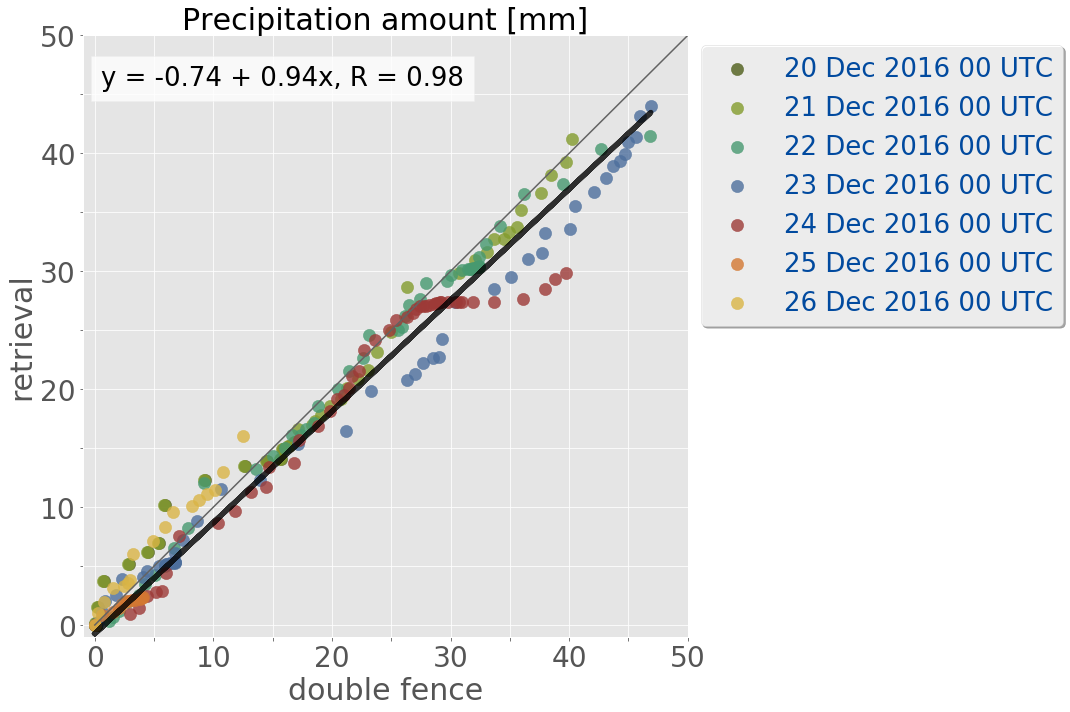
\includegraphics[trim={0.cm 0.cm 13cm 0cm},clip,
		width=\textwidth]{./fig_obs_ret/obs_ret_20161220_26_00}
		\caption{}\label{fig:res:obs_ret_scatter}
	\end{subfigure}
	%
	\begin{subfigure}[b]{0.59\textwidth}
		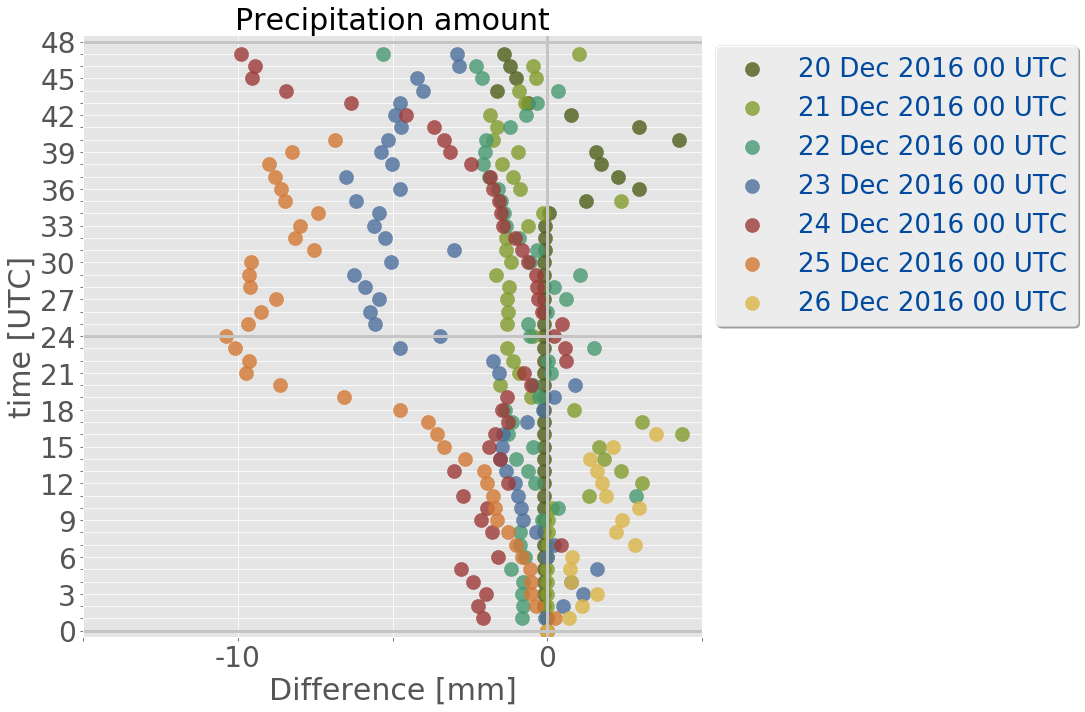
\includegraphics[trim={0.cm 0.cm 0cm 0cm},clip,
		width=\textwidth]{./fig_obs_ret/diff_20161220_26_00}
		\caption{}\label{fig:res:diff_ret_scatter}
	\end{subfigure}
	% label
	%    \begin{subfigure}[t]{0.18\textwidth}
	%   	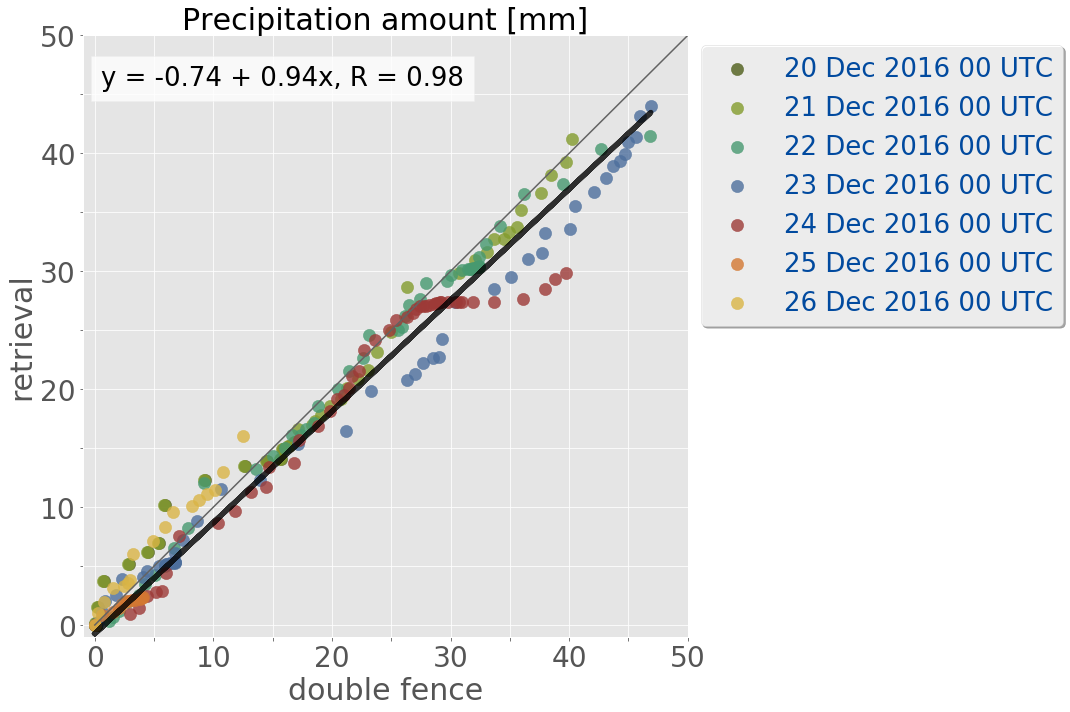
\includegraphics[trim={25.cm 13.cm 0cm 1.3cm},clip,
	%  width=\textwidth]{./fig_obs_ret/obs_ret_20161220_26_00}
	% \end{subfigure}
	\caption{\protect\subref{fig:res:obs_ret_scatter}: Surface precipitation amount comparison between the double fence observations and the retrieved surface accumulation of precipitation for \SI{48}{\hour}. In black the linear correlation between the double fence observations and retrieved surface snow. 
		\protect\subref{fig:res:diff_ret_scatter}: Difference between the retrieved and the observed accumulation by the double fence. The colours represent the different starting days at \SI{0}{\UTC} for the \SI{48}{\hour} accumulation.}\label{fig:res:obs_ret}
\end{figure}
%%%%%%%%%%%%%%%%%%%%%%%%%%%%%%%%%%%%%%%%%%%%%%
\\
\\
Similar to this study, \citet{cooper_variational_2017} used a CloudSat snow particle model, PSD and fall speed from MASC observations for five snow events at Barrow, Alaska. The comparison to the weather station revealed a difference between National Weather Service observations and retrieved accumulations of \SI{- 18}{\percent} for five snow events.
%%%%%%% table error sfc acc ret obs %%%%%%%%%%%%%%%%
\begin{table}[t!]
	\begin{center}
		\caption{Comparison of observed (obs.) and retrieved (ret.) snow amounts for the Christmas storm 2016. Difference refers to the difference of the retrieved and observed snow accumulation after \SI{12}{\hour} and \SI{24}{\hour}. The average difference is the value over all six/four days. Excluding values after \SI{12}{\UTC} on \SI{25}{\dec} and after \SI{17}{\UTC} on \SI{26}{\dec}.}\label{tab:res:ret_error}
		\begin{tabular}{c||r|r|c|c||r|r|c|c}
			\hline \hline
			& \multicolumn{4}{c||}{\textbf{\SI{12}{\hour} accumulation}} & \multicolumn{4}{c}{\textbf{\SI{24}{\hour} accumulation}}    \\ \cline{2-9}
			\textbf{Day} & \multicolumn{2}{c|}{\textbf{Amount}} & \textbf{Difference} & \textbf{Average} &  \multicolumn{2}{c|}{\textbf{Amount}} & \textbf{Difference} & \textbf{Average}  \\\cline{2-3} \cline{6-7}
			\textbf{in 2016} & \textbf{obs.} & \textbf{ret.} & & \textbf{difference} & \textbf{obs.} & \textbf{ret.} & & \textbf{difference} \\\cline{2-9}
			& \multicolumn{2}{c|}{[\SI{}{\mm}]} & [\SI{}{\percent}] & [\SI{}{\percent}] & \multicolumn{2}{c|}{[\SI{}{\mm}]} & [\SI{}{\percent}] & [\SI{}{\percent}] \\ \hline\hline
			%		\num{20} Dec & \num{0.1} &\num{0.0} & \num{-97.8} & & \num{0.1} & \num{0.0} & \num{- 97.8} &  \\\cline{1-9}
			\num{21} Dec & \num{0.7} & \num{3.8} & +\num{435.8} &  & \num{17.1} & \num{16.6} & \num{-2.7} & \multirow{4}{*}{\num{-4.7}}   \\\cline{1-5}\cline{6-8}
			\num{22} Dec & \num{13.6}& \num{13.2} & \num{- 3.0} & \multirow{5}{*}{\num{-2.1}} & \num{25.6} &\num{25.1} & \num{-2.1} &   \\\cline{1-4}\cline{6-8}
			\num{23} Dec & \num{6.3} &\num{5.2} & \num{- 16.8} & & \num{23.3}& \num{19.8} & \num{-14.9} &   \\\cline{1-4}\cline{6-8}
			\num{24} Dec & \num{14.7} & \num{13.4} & \num{- 8.6} && \num{24.8} & \num{25.0} & +\num{0.8} &   \\\cline{1-4}\cline{6-9}
			\num{25} Dec &  \num{4.3} & -- & -- & & +\num{15.4} & -- & -- & \\\cline{1-4}\cline{6-9}
			\num{26} Dec & \num{8.8} & \num{10.6} & +\num{20.1} &  &  \num{25.1} &-- & -- &  \\\hline\hline
		\end{tabular}
	\end{center}
\end{table}
%%%%%%%%%%%%%%%%%%%%%%%%%%%%%%%%%%%%%%%%%%%%%%
\\
\Cref{tab:res:ret_error} shows the difference for each individual day and the average difference for six and four days, depending on the accumulation of \SI{12}{\hour} or \SI{24}{\hour}.
The choice of the correct PSD model, slope parameters and fall speed in the optimal estimation snowfall retrieval, shows a good agreement with the observations at Haukeliseter for the 2016 Christmas storm in contrast to the \SI{200}{\percent} difference when only using the CloudSat snowfall algorithm (\Cref{sec:retrieval}). It also indicates a reduction of the non-uniqueness of snow accumulation is reduced, when using a combination of ground-based observations instead of only Ze-S relationships. 
%Of course, more storms should be investigated to find the exact correlation between the surface observations and the estimated accumulation to see if the deviation keeps as small for different snow patterns at Haukeliseter. 
%During the 2016 Christmas storm the average error for \SI{24}{\hour} accumulation is almost similar to the best estimate at Barrow, Alaska. 
\\
It turns out that there is no relation between high and low precipitation events since the differences vary daily. \citet{cooper_variational_2017} also showed different combinations of PSD assumptions and snow fall speed. For Barrow, best agreements between observations and retrieved snow accumulation were found by using the CloudSat particle model, slope parameters and snowfall speeds from the MASC. In the here presented study, the best assumption for surface snow accumulation was found by using a particle model for rimed aggregates (\Cref{sec:retrieval} and \ref{sec:ret:sensitivity}) such as in \Cref{fig:ret:all_part}. 
\\
\\
On \SI{21}{\dec}, the deviation is large (\SI{435.8}{\percent}). This is probably related to an observation of precipitation at the double fence, while the MRR did not observe precipitation.
On \SI{21}{\dec}, observation at the double fence might be related to some particles stirred up by wind into the orifice of the gauge. Since no manual observations are done at the Haukeliseter site, is it difficult to say if blowing snow occurred or if it was snowing. This introduces additional errors on the double fence measurements. From the vertical MRR reflectivity, in \Cref{sec:res:large_scale_vert}, \Cref{fig:ret:refl}, it can be seen, that precipitation was not observed on \SI{21}{\dec} before \SI{9}{\UTC}.
\\
Even though it is assumed that the double fence is the correct measurement, there are still some uncertainties, such as under-catch during high wind speeds \citep[][unpublished]{wolff_wmo_2018}. 
A better way to examine the accuracy of the retrieved surface precipitation accumulation could be to compare the results to measurements inside a bush gauge. 
\\
\citet{wolff_wmo_2018}, [unpublished] estimates the under-catchment of double fence gauge compared to bush gauge measurements to \SI{10}{\percent}, for outside winds of \SI{9}{\mPs} (\Cref{sec:dofe}).
If the double fence gauge underestimate frozen precipitation under high wind condition, would follow that the optimal estimation retrieval results are more than \SI{20}{\percent} too low to the true state. 
\\
During the Christmas 2016 event the average difference is low for \SI{24}{\hour} surface accumulation (\SI{-4.7}{\percent}) in \Cref{tab:res:ret_error}. At Barrow, Alaska, the best average difference between retrieved and observed surface accumulation was \SI{36}{\percent} \citep{cooper_variational_2017}.
%Anyway, the low average difference value for \SI{24}{\hour} accumulation, in \Cref{tab:res:ret_error} during the Christmas 2016 event (\SI{-4.7}{\percent}) follow a much lower average difference between retrieved and observed surface accumulation than at Barrow (\SI{36}{\percent}). 
This leads to a very good agreement between observed and retrieved snow accumulation during \num{21} to \SI{24}{\dec}. 
In \Cref{sec:res:large_scale_vert}, the vertical SWC will be compared to the forecasted MEPS values for the 2016 Christmas storm. Despite the under-catchment of snow in high wind speeds, the double fence measurement give trust for the retrieved profiles of snow water content. While snow water content is compared to the MEPS forecast, it should be kept in mind that retrieved snow accumulation is underestimated and therefore the vertical SWC may be too low.
%influenced by wind will the small average difference for \num{21} to \SI{24}{\dec} give confidence in the retrieved profiles of snow water content when comparing to the forecast, but it should be kept in mind that retrieved snow accumulation is underestimated and therefore may the vertical SWC be too low.
%%%%%%%%%%%%%%%%%%%%%%%%%%%%%%%%%%%%%%%%%%%%%%%%%%%%%%%%%%%%%%%%%%%%%%%%%%











%%%%%%%% Overestimation of surface snowfall %%%%%%%%%%%%%%
\subsection{Comparison of Surface Observation and MEPS}\label{sec:sfc_acc}
Hereafter, MEPS surface precipitation prediction forecast is compared to the double fence gauge observations at Haukeliseter to see if observed surface accumulation was correctly predicted by MEPS.
%%% image surface accumulation %%%%%%%%%%%%%%%%%%%%%%%%%%%%%%%%%%%%%
\begin{figure}[H]
	\centering
	% 21/12
	\begin{subfigure}[t]{0.97\textwidth}		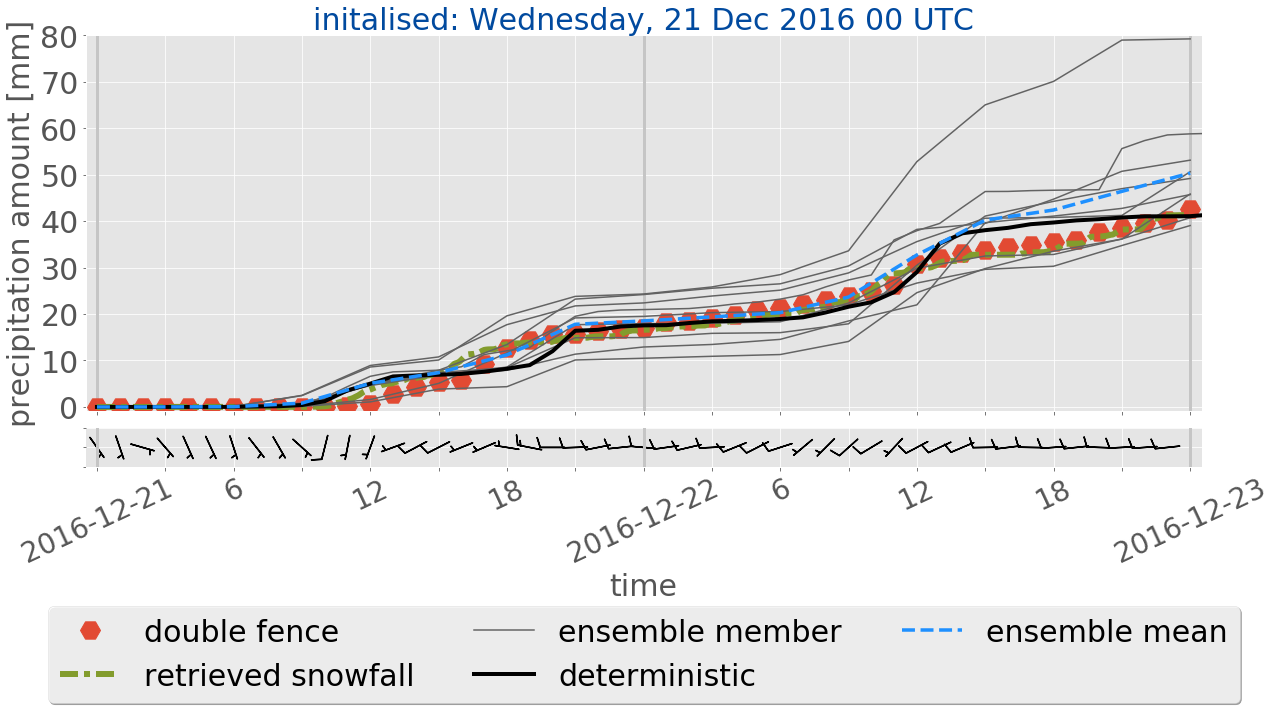
\includegraphics[trim={0.cm 5.2cm 0.cm 0cm},clip,width=\textwidth]{./fig_sfc_acc/acc_wind_20161221_00}
		\caption{}\label{fig:sfc_acc21}
	\end{subfigure}
	% 22/12
	\begin{subfigure}[t]{0.97\textwidth}		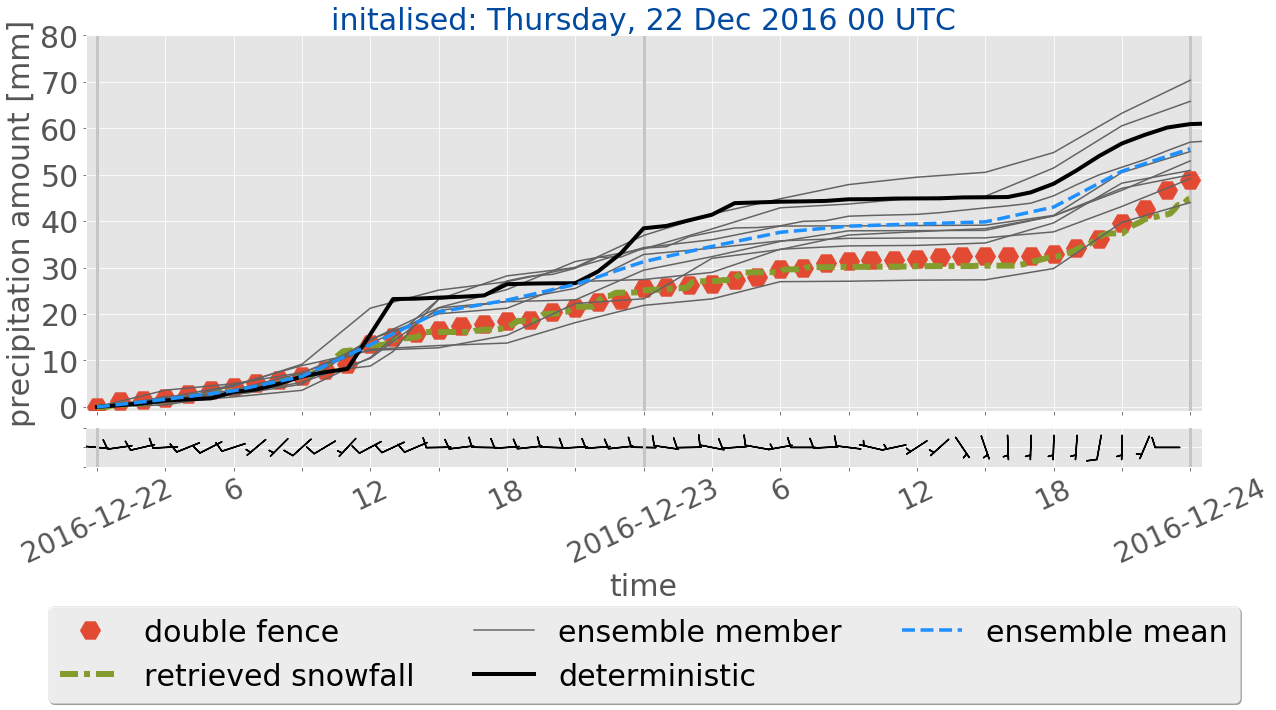
\includegraphics[trim={0.cm 5.2cm 0.cm 0cm},clip,width=\textwidth]{./fig_sfc_acc/acc_wind_20161222_00}
		\caption{}\label{fig:sfc_acc22}
	\end{subfigure}
	% 23/12
	\begin{subfigure}[t]{0.97\textwidth}	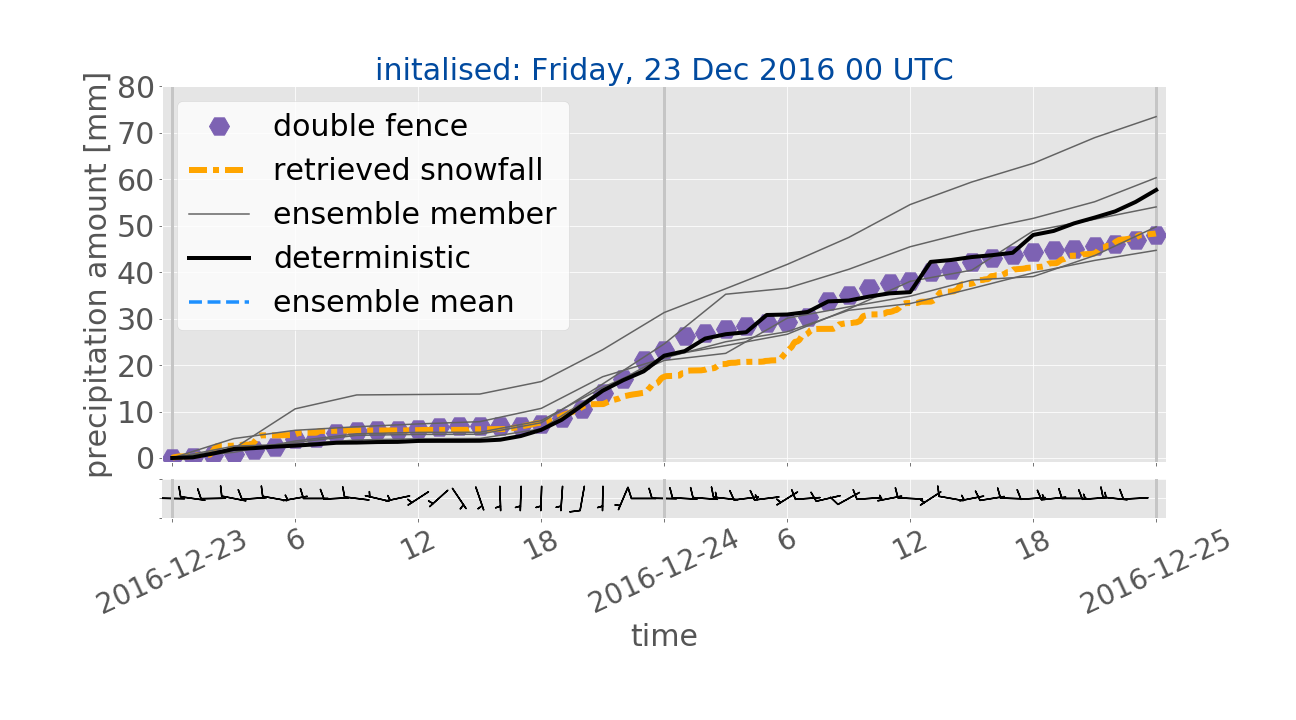
\includegraphics[trim={0.cm 5.2cm 0.cm 0cm},clip,width=\textwidth]{./fig_sfc_acc/acc_wind_20161223_00}
		\caption{}\label{fig:sfc_acc23}
	\end{subfigure}
	% label
	\begin{subfigure}[t]{\textwidth}
		\centering
		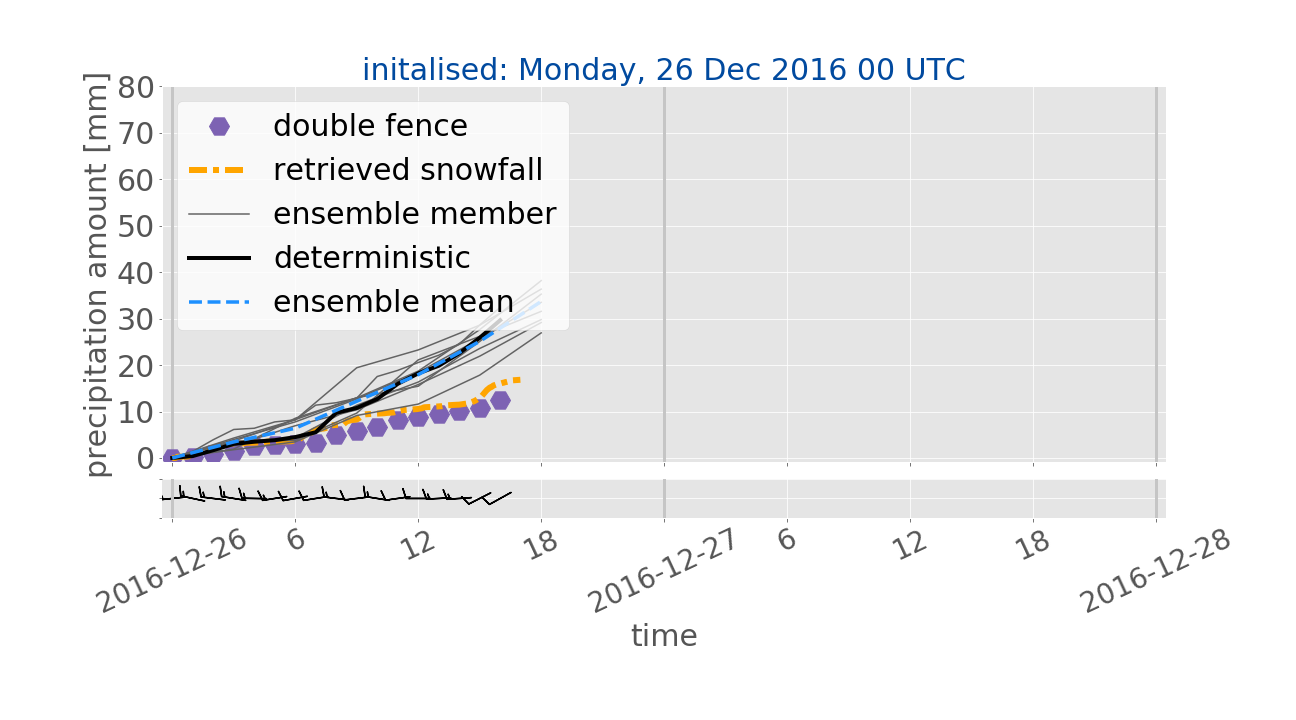
\includegraphics[trim={1.2cm 0cm 1.1cm 21.4cm},clip,width=0.8\textwidth]{./fig_sfc_acc/acc_wind_20161226_00}
	\end{subfigure}
	\caption{\SI{48}{\hour} surface precipitation accumulation for \num{21} to \SI{23}{\dec}. Representing the values from the double fence in red, hexagons; optimal estimation retrieval output at the first noise free level
		%snow layer height \SI{400}{\metre} 
		in dash-dotted green; MEPS ensemble member deterministic forecast, initialised at \SI{00}{\UTC} in black and its nine perturbed ensemble members in grey. The ensemble mean of all ten members is shown in dashed blue. Underneath is the associated last hour \SI{10}{\minute} average wind from the weather mast at \SI{10}{\metre} height. }\label{fig:sfc_acc:2123}
\end{figure}
\begin{figure}[H]%\ContinuedFloat
	\centering
	% 24/12
	\begin{subfigure}[t]{0.97\textwidth}			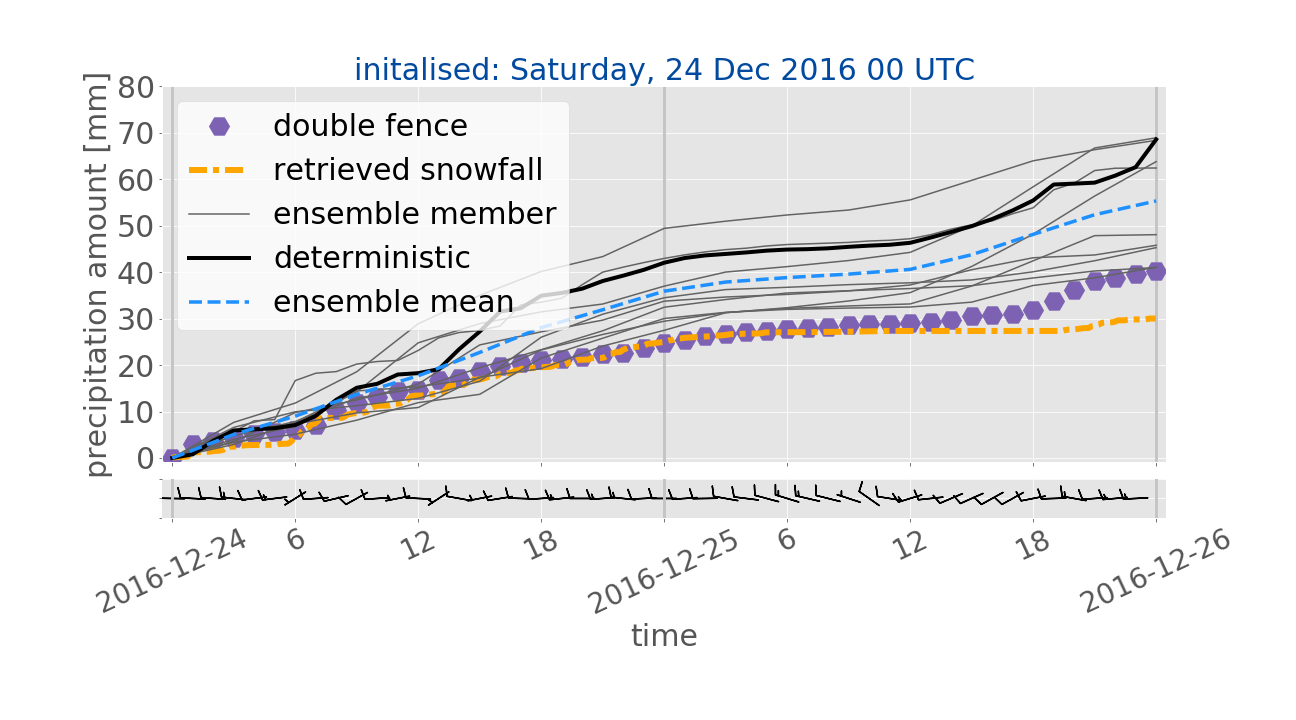
\includegraphics[trim={0.cm 5.2cm 0.cm 0cm},clip,width=\textwidth]{./fig_sfc_acc/acc_wind_20161224_00}
		\caption{}\label{fig:sfc_acc24}
	\end{subfigure}
	% 25/12
	\begin{subfigure}[t]{0.97\textwidth}
		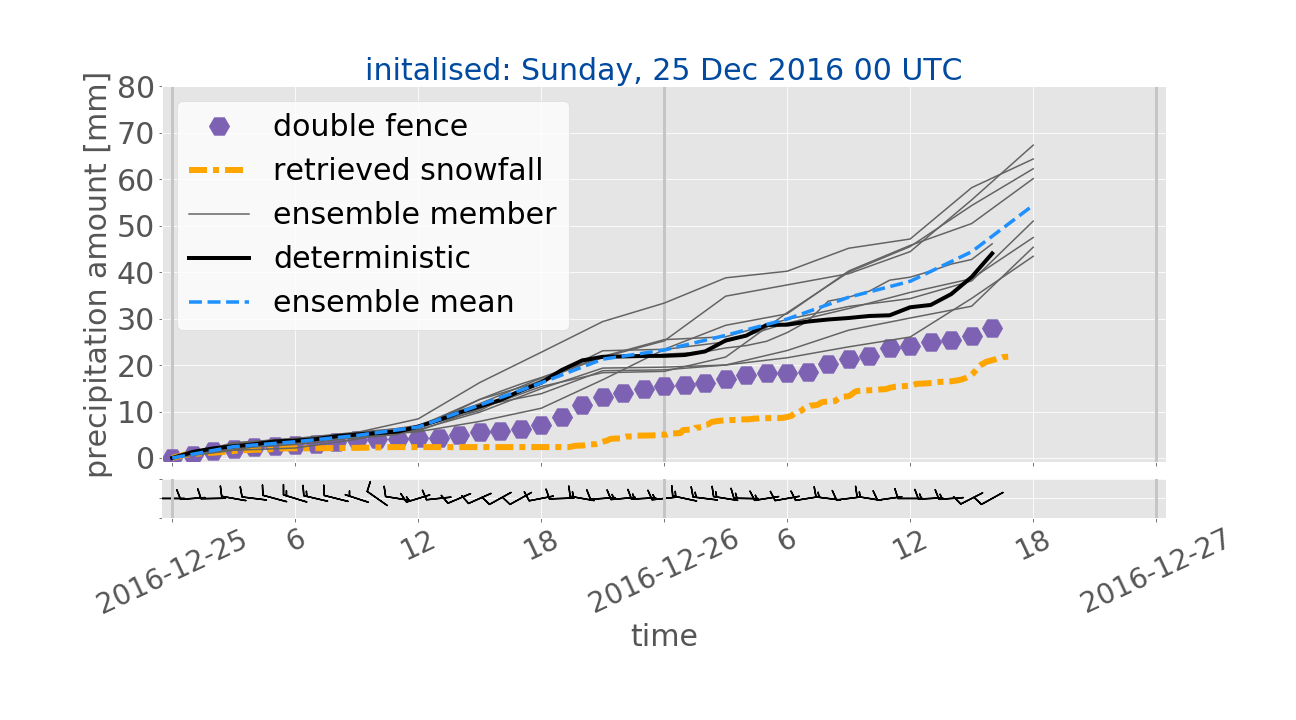
\includegraphics[trim={0.cm 3.6cm 0.cm 0cm},clip,width=\textwidth]{./fig_sfc_acc/acc_wind_20161225_00}
		\caption{}\label{fig:sfc_acc25}
	\end{subfigure}
	% 26/12
	\begin{subfigure}[t]{0.97\textwidth}	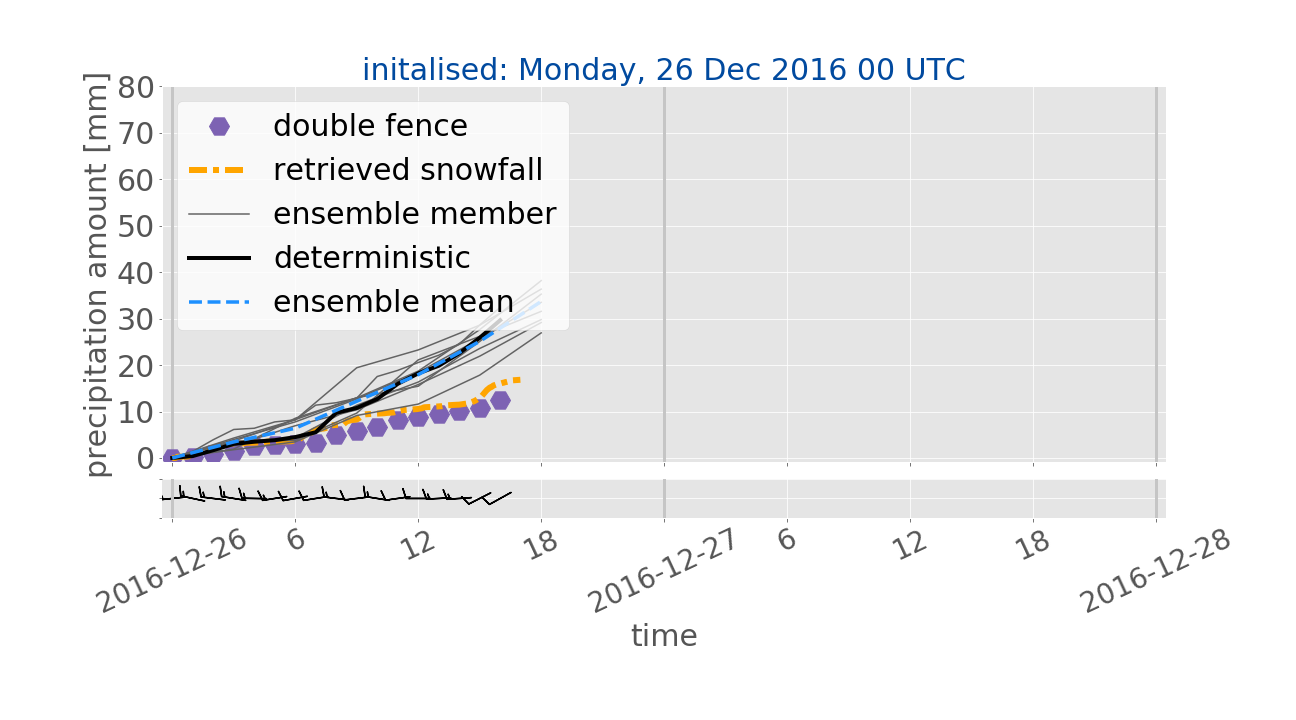
\includegraphics[trim={0.cm 3.6cm 0.cm 0cm},clip,width=\textwidth]{./fig_sfc_acc/acc_wind_20161226_00}
		\caption{}\label{fig:sfc_acc26}
	\end{subfigure}
	% label
	\begin{subfigure}[t]{\textwidth}
		\centering
		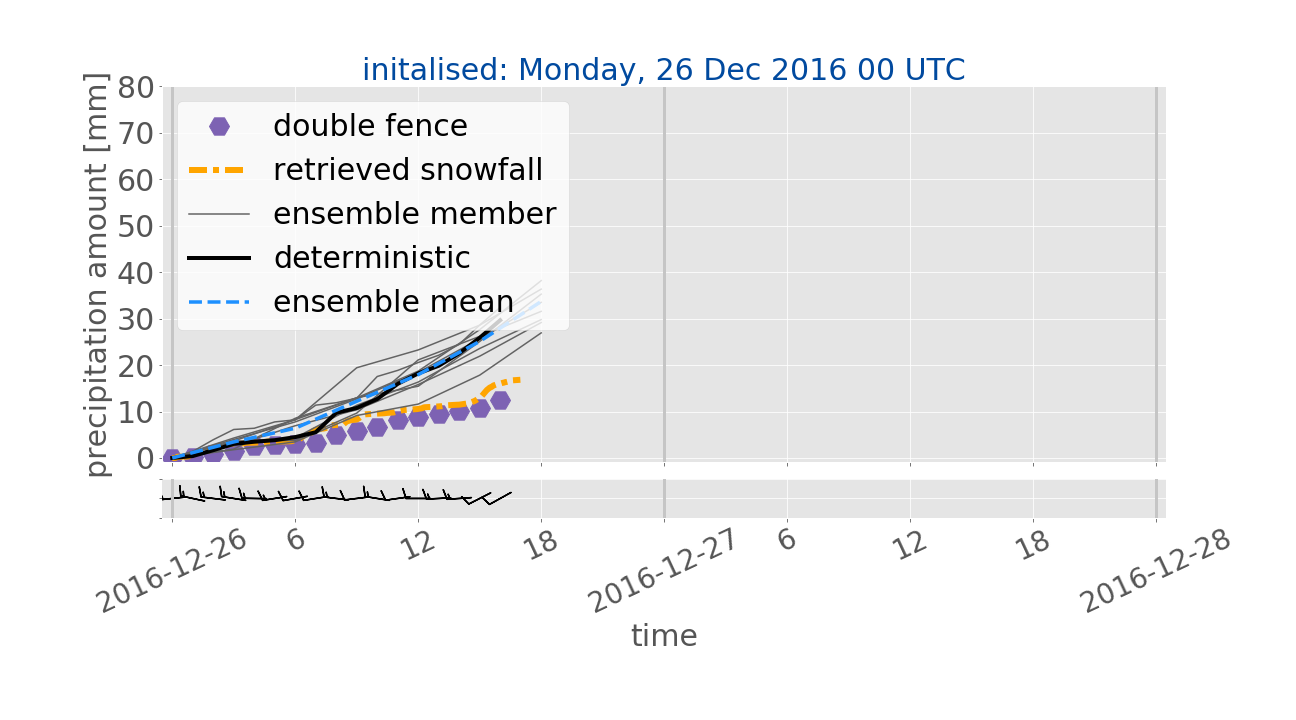
\includegraphics[trim={1.2cm 0cm 1.1cm 21.4cm},clip,width=0.8\textwidth]{./fig_sfc_acc/acc_wind_20161226_00}
	\end{subfigure}
	\caption{\textit{(As \Cref{fig:sfc_acc:2123}.)} Initialisations on \num{24}, \num{25}, and \SI{26}{\dec} at \SI{00}{\UTC}. }\label{fig:sfc_acc:2426}
\end{figure}
%%%%%%%%%%%%%%%%%%%%%%%%%%%%%%%%%%%%%%%%%%%%%%%%%%%%%%%%%%%%%%%%%%%%%%%%%%
\noindent
\\
%%% sfc dofe comparison %%%%%
\Cref{fig:sfc_acc} shows surface accumulation observations at the double fence, retrieved snow accumulation, and MEPS forecast for \SI{48}{\hour}.  
The blue dashed line shows the ensemble mean of all ten members. The ensemble mean of precipiation amount is calculated every three hours, due to the three hourly time resolution of most of the perturbed member (\Cref{sec:ens_mean_spread}).
When not all perturbed member forecast data was available from the \citet{norwegian_meteorological_institute_met_2016}, like on \SI{23}{\dec} (\Cref{fig:sfc_acc23}), no ensemble mean is calculated. 
At the bottom of \Cref{fig:sfc_acc} the associated \SI{10}{\minute} average wind of the last hour from the \SI{10}{\metre} weather mast at Haukeliseter is presented. This will help to see if surface precipitation observations by the double fence may be influenced by wind. MEPS surface accumulation does not account for undercatchment by too high wind speeds, and therefore are not presented in \Cref{fig:sfc_acc}.
\\
In general, \Cref{fig:sfc_acc21,fig:sfc_acc22,fig:sfc_acc23} show a better agreement between double fence precipitation amount observations and forecast for \SI{48}{\hour} forecasts initialised on \num{21} to \SI{23}{\dec} at \SI{0}{\UTC} than for initialisations on \num{24} to \SI{26}{\dec}. 
The double fence observation lie for \num{21}, \num{22}, and \SI{23}{\dec} within the spread of the ensemble members (\Cref{fig:sfc_acc21,fig:sfc_acc22,fig:sfc_acc23}), covering the uncertainty within the measurements (\Cref{sec:DIM:MEPS}). On the other hand, observations between \num{24} and \SI{26}{\dec} are too low  compared to the ensemble spread (\Cref{fig:sfc_acc24,fig:sfc_acc25,fig:sfc_acc26}).
During \num{24} and \SI{26}{\dec}, the low-pressure system intensifies and gets closer to the Norwegian coast, influencing the local weather in Norway (\Cref{sec:largeScale}). \Cref{fig:sfc_acc24} to \subref{fig:sfc_acc26} indicate a larger estimated surface precipitation amount for all ten ensemble members compared to observed values at the measurement site between \num{24} to \SI{26}{\dec}. Furthermore, all ensemble members seem to overestimate the surface accumulation after \SI{18}{\hour} on \SI{24}{\dec} and after \SI{12}{\hour} on \num{25} and \SI{26}{\dec}. 
\\
%%% Correlation %%%%%
The correlation for precipitation between \SI{48}{\hour} double fence observation and ensemble precipitation forecast is presented in \Cref{fig:scat:precip2123} and \subref{fig:scat:precip2426}. Showing a better agreement for \num{21} to \SI{23}{\dec} than initialisation on \num{24} to \SI{26}{\dec}. On \num{21} to \SI{23}{\dec} the slope of the regression line is relatively close to unity. 
%indicating a good agreement between MEPS forecast and the observations by the double fence.
%On \num{24} and \SI{26}{\dec} the mean absolute error for the \SI{12}{\hour} surface accumulation in \Cref{fig:MAE:precip12} is largest with values up to \SI{15}{\mm}. 
\\
% description each day overestimation plot
%%% 24/12
Initialisations on \SI{24}{\dec} (\Cref{fig:sfc_acc24}) indicate an overestimation of the deterministic surface snow amount prediction already after \SI{13}{\hour} forecast time. The deterministic forecast in solid black in \Cref{fig:sfc_acc24} is much higher and increases faster than the observations and the nine perturbed members. In \Cref{fig:sfc_acc24} at \SI{16}{\UTC}, a difference of approximately \SI{15}{\mm} can be seen when compared to the surface measurements. This difference remains almost constant over the forecast time. 
\\
%%% 25/12
While the cyclone propagates closer to Norway, the forecast error of the surface precipitation increases. Overestimation occurs around \SI{12}{\UTC} on \SI{25}{\dec}. This overestimation of the precipitation amount could be associated with the warm sector evolution at Haukeliseter (\Cref{sec:res:large_scale_sfc}). Afterwards, with increasing lead time MEPS forecasts show the same simulated precipitation development as the double fence, but too high. The precipitation is light between \SIlist{12;18}{\UTC} which shows as an almost constant surface precipitation amount. At \SI{18}{\UTC} the surface precipitation amount at the double fence increases and so does the MEPS forecast.
%%% 26/12
An overestimation of the surface precipitation is also simulated on \SI{26}{\dec}. While the surface analysis indicates the passage of an occlusion after \SI{15}{\UTC} (\Cref{fig:DT26}, \ref{fig:GP26}, and \Cref{sec:res:large_scale_sfc}). The overestimation seems to occur after a \SI{12}{\hour} lead time in \Cref{fig:sfc_acc26}. 
The MEPS ensemble seems to predict the timing of precipitation correctly compared to the double fence, but estimates a too high surface accumulation.
%%%%%%% table error MEPS accumulation %%%%%%%%%%%%%%%%
\begin{table}[t]
	\begin{center}
		\caption{Observations (obs.) and forecasted (MEPS) surface precipitation amounts for the Christmas storm 2016. Difference refers to the percentage difference between MEPS ensemble members and the double fence observation, averaged over all ensemble member for \SIlist{12;24}{\hour}. The average difference is the value over all days.}\label{tab:res:MEPS_err}
		\begin{tabular}{c||r|r|c|c|c||r|r|c|c|c}
			\hline \hline
			& \multicolumn{5}{c||}{\textbf{\SI{12}{\hour} accumulation}} & \multicolumn{5}{c}{\textbf{\SI{24}{\hour} accumulation}}    \\ \cline{2-11}
			\textbf{Day} & \multicolumn{2}{c|}{\textbf{Amount}} & \textbf{Difference} & \multicolumn{2}{c||}{\textbf{Average}} &  \multicolumn{2}{c|}{\textbf{Amount}} & \textbf{Difference} & \multicolumn{2}{c}{\textbf{Average}}  \\\cline{2-3} \cline{7-8}
			\textbf{in 2016} & \textbf{obs.} & \textbf{MEPS} & & \multicolumn{2}{c||}{\textbf{difference}} & \textbf{obs.} & \textbf{MEPS} & & \multicolumn{2}{c}{\textbf{difference}} \\\cline{2-11}
			& \multicolumn{2}{c|}{[\SI{}{\mm}]} & [\SI{}{\percent}] & \multicolumn{2}{c||}{ [\SI{}{\percent}]} & \multicolumn{2}{c|}{[\SI{}{\mm}]} & [\SI{}{\percent}] & \multicolumn{2}{c}{ [\SI{}{\percent}]} \\ \hline\hline
			%			\num{20} Dec & \num{0.1} &\num{0.4} & +\num{290.7} & & &\num{0.1} & \num{0.4} & +\num{302.1} & & \\\cline{1-11}
			\num{21} Dec & \num{0.7} & \num{5.1} & +\num{626.1} &  &\multirow{6}{*}{+\num{134.7}} & \num{17.1} & \num{18.5} & +\num{8.3} & \multirow{3}{*}{+\num{10.8}}& \multirow{6}{*}{+\num{32.6}}   \\\cline{1-5}\cline{7-9} 
			\num{22} Dec & \num{13.6} & \num{13.4} & \num{-1.6} & \multirow{2}{*}{+\num{1.3}} & & \num{25.6} & \num{31.3} & +\num{22.2} &  &  \\\cline{1-4}\cline{7-9}
			\num{23} Dec & \num{6.3} & \num{6.6} & +\num{4.2} & & & \num{23.3} & \num{23.7} & +\num{1.8} &  &  \\\cline{1-5}\cline{7-10}
			\num{24} Dec & \num{14.7} & \num{17.7} & +\num{20.4} & \multirow{3}{*}{+\num{59.8}} & & \num{24.8} & \num{35.9} & +\num{44.8} & \multirow{3}{*}{+\num{54.4}}  &  \\\cline{1-4}\cline{7-9}
			\num{25} Dec & \num{4.3} & \num{6.7} & +\num{55.1} & & & \num{15.4} & \num{23.3} & +\num{50.8} & &   \\\cline{1-4}\cline{7-9}
			\num{26} Dec & \num{8.8} & \num{17.9} & +\num{104.0} & & & \num{25.1} & \num{42.1} & +\num{67.5} &  &  \\\hline\hline
		\end{tabular}
	\end{center}
\end{table}
%%%%%%%%%%%%%%%%%%%%%%%%%%%%%%%%%%%%%%%%%%%%%%%%%%%%%%%%%%%%%%%%%%%%%%%%%%
%%% average difference
\noindent
\Cref{tab:res:MEPS_err} shows the difference between the observations and ensemble mean MEPS forecast for \SIlist{12;24}{\hour} accumulation. Generally the forecast accuracy decreases with lead time which can be seen on the larger deviation between the ensemble member after \SI{18}{\hour} lead time (\Cref{fig:sfc_acc:2123}, \ref{fig:sfc_acc:2426}). As seen in \Cref{tab:res:MEPS_err}, the average difference decreases with longer forecast time. For \num{21} to \SI{26}{\dec} the deviation is +\SI{134.7}{\percent}. For longer lead times, \SI{24}{\hour}, the average difference is reduced to +\SI{32.6}{\percent}. Due to the good forecast between \num{21} to \SI{23}{\dec} ($\le$ \SI{11}{\percent}) the averaged difference is smaller. 
\\
On \SI{21}{\dec} very large deviation (\SI{626.1}{\percent}) is shown. 
AROME-MetCoOp had problems with too low precipitation. The deviation between observed and forecasted values was larger if the precipitation amount is less than \SI{10}{\mm} \citep{muller_arome-metcoop:_2017}. At Haukeliseter, low precipitation amount is observed (\SI{0.7}{\mm}) on \SI{21}{\dec}.
%This error is related to the small precipitation amount (\SI{0.7}{\mm}) observations at Haukeliseter, which is a known difficulty for precipitation forecasts \citep{muller_arome-metcoop:_2017}. 
The daily percent difference show to be high for the last three days of the 2016 Christmas extreme event.  
\\
%%% ME, MAE
The largest overestimation of MEPS forecast for precipitation amount is seen in \Cref{tab:res:MEPS_err} on \SI{26}{\dec} with +\SI{104}{\percent} for \SI{12}{\hour}. This shows the highest overestimation for the three days (\num{24} to \SI{26}{\dec}).
\\
In \Cref{fig:bias} show the ensemble member a balanced bias from \num{21} to \SI{23}{\dec}. The bias for \num{24} to \SI{26}{\dec} is wet, also showing the overestimation of surface accumulation.
In \Cref{fig:MAE:precip12}, the mean absolute error is less than \SI{7}{\mm} for \num{21} to \SI{23}{\dec} and increases with intensification of the storm up to \SI{14}{\mm} on \SI{26}{\dec}. The mean absolute error in \Cref{fig:MAE:precip12} for \SI{12}{\hour} precipitation is less than \SI{7}{\mm} on \SI{25}{\dec}, similar to \num{21} to \SI{23}{\dec}.
%%%%%%% table if 10% underestimate of double fence %%%%%%%%%%%%%%%%
\begin{table}[t]
	\begin{center}
		\caption{ \textit{AS \Cref{tab:res:MEPS_err}}, adjusted just for an under-catchment of \SI{10}{\percent} difference by the double fence gauge. }\label{tab:res:MEPS_err_10}
		\begin{tabular}{c||r|r|c|c|c||r|r|c|c|c}
			\hline \hline
			& \multicolumn{5}{c||}{\textbf{\SI{12}{\hour} accumulation}} & \multicolumn{5}{c}{\textbf{\SI{24}{\hour} accumulation}}    \\ \cline{2-11}
			\textbf{Day} & \multicolumn{2}{c|}{\textbf{Amount}} & \textbf{Difference} & \multicolumn{2}{c||}{\textbf{Average}} &  \multicolumn{2}{c|}{\textbf{Amount}} & \textbf{Difference} & \multicolumn{2}{c}{\textbf{Average}}  \\\cline{2-3} \cline{7-8}
			\textbf{in 2016} & \textbf{obs.} & \textbf{MEPS} & & \multicolumn{2}{c||}{\textbf{difference}} & \textbf{obs.} & \textbf{MEPS} & & \multicolumn{2}{c}{\textbf{difference}} \\\cline{2-11}
			& \multicolumn{2}{c|}{[\SI{}{\mm}]} & [\SI{}{\percent}] & \multicolumn{2}{c||}{ [\SI{}{\percent}]} & \multicolumn{2}{c|}{[\SI{}{\mm}]} & [\SI{}{\percent}] & \multicolumn{2}{c}{ [\SI{}{\percent}]} \\ \hline\hline
			%			\num{20} Dec & \num{0.1} &\num{0.4} & +\num{251.6} & & &\num{0.1} & \num{0.4} & +\num{261.9} & & \\\cline{1-11}
			\num{21} Dec & \num{0.8} & \num{5.1} & +\num{553.5} &  &\multirow{6}{*}{+\num{111.2}} & \num{19.0} & \num{18.5} & -\num{2.5} & \multirow{3}{*}{-\num{0.3}}& \multirow{6}{*}{+\num{19.3}}   \\\cline{1-5}\cline{7-9} 
			\num{22} Dec & \num{15.1} & \num{13.4} & \num{-11.4} & \multirow{2}{*}{\num{-8.8}} & & \num{28.4} & \num{31.3} & +\num{9.9} &  &  \\\cline{1-4}\cline{7-9}
			\num{23} Dec & \num{7.0} & \num{6.6} & -\num{6.2} & & & \num{25.9} & \num{23.7} & -\num{8.4} &  &  \\\cline{1-5}\cline{7-10}
			\num{24} Dec & \num{16.3} & \num{17.7} & +\num{8.4} & \multirow{3}{*}{+\num{43.8}} & & \num{27.6} & \num{35.9} & +\num{30.3} & \multirow{3}{*}{+\num{39.0}}  &  \\\cline{1-4}\cline{7-9}
			\num{25} Dec & \num{4.8} & \num{6.7} & +\num{39.6} & & & \num{17.1} & \num{23.3} & +\num{35.8} & &   \\\cline{1-4}\cline{7-9}
			\num{26} Dec & \num{9.8} & \num{17.9} & +\num{83.6} & & & \num{27.9} & \num{42.1} & +\num{50.8} &  &  \\\hline\hline
		\end{tabular}
	\end{center}
\end{table}
%%%%%%%%%%%%%%%%%%%%%%%%%%%%%%%%%%%%%%%%%%%%%%%%%%%%%%%%%%%%%%%%%%%%%%%%%%
\noindent
\\
%%% average difference with 10%
Since MEPS performance was better on \num{21} to \SI{23}{\dec} one might assume that the double fence measurement is influenced by surface winds. 
%\citet{wolff_wmo_2018}, [unpublished] states that the double fence gauge is influenced by wind, and that the double fence gauge underestimates precipitation accumulation within \SI{10}{\percent} for winds up to \SI{9}{\mPs}. 
A relation between high wind and double fence observation could be possible. \Cref{tab:res:MEPS_err_10} presents the percentage difference between the double fence and MEPS forecasts under the condition that the double fence is affected by wind with a catch-ratio less than \SI{10}{\percent}. Here, it also shows an increase in forecast accuracy for precipitation accumulation over \SI{24}{\hour}.
%, but a reduction of overestimation for surface accumulation in general. 
The average difference is reduced by \SI{23.5}{\percent} for \SI{12}{\hour} accumulation. Assuming an accumulation underestimation of \SI{10}{\percent} would lead to a reduction of overestimation to \SI{43.8}{\percent} for \SI{12}{\hour} during \num{24} to \SI{26}{\dec} (\Cref{tab:res:MEPS_err_10}).
This shows that even with a \SI{10}{\percent} under-catchment from the double fence gauge, MEPS would still overestimate the surface accumulation (\SI{12}{\hour}: +\SI{43.8}{\percent}; \SI{24}{\hour}: +\SI{39}{\percent}). 
\\
%%% 24, 25, 26/12
On \num{24}, \num{25}, and \SI{26}{\dec} winds between \SIlist{5;18}{\mPs} were observed (\Cref{fig:res:sfc_ws23}, \ref{fig:res:sfc_ws25}, \ref{fig:res_sf_ws26}). The accumulation after \SI{12}{\hour} lead time in \Cref{tab:res:MEPS_err_10} indicate if wind may have influenced the catchment of the double fence and effect the result of overestimation. It shows, overestimation would still be present on \num{25} and \SI{26}{\dec}. On the other hand, overestimation would not be present for \SI{24}{\dec} until \SI{12}{\hour} accumulation.
\\
Still, an simulation of too much surface accumulation is apparent for \SI{24}{\hour} lead time.
It seems even though the double fence gauge is influenced by wind, the overestimation of surface accumulation by MEPS is still present. 
% The surface wind observation in \Cref{fig:res:sfc_ws26} shows also high wind speed up to \SI{17.5}{\mPs} observations on \SI{26}{\dec}.  The application of the \SI{10}{\percent} under-catchment on the double fence observation would still follow an error of \SI{83.6}{\percent} (\Cref{tab:res:MEPS_err,tab:res:MEPS_err_10}).
\\
%%% image surface accumulation variation %%%%%%%%%%%%%%%%%%%%%%%%%%%%%%%%%%%%%
\begin{figure}[h!]
	\centering
	\begin{subfigure}[b]{\textwidth}
		\centering
		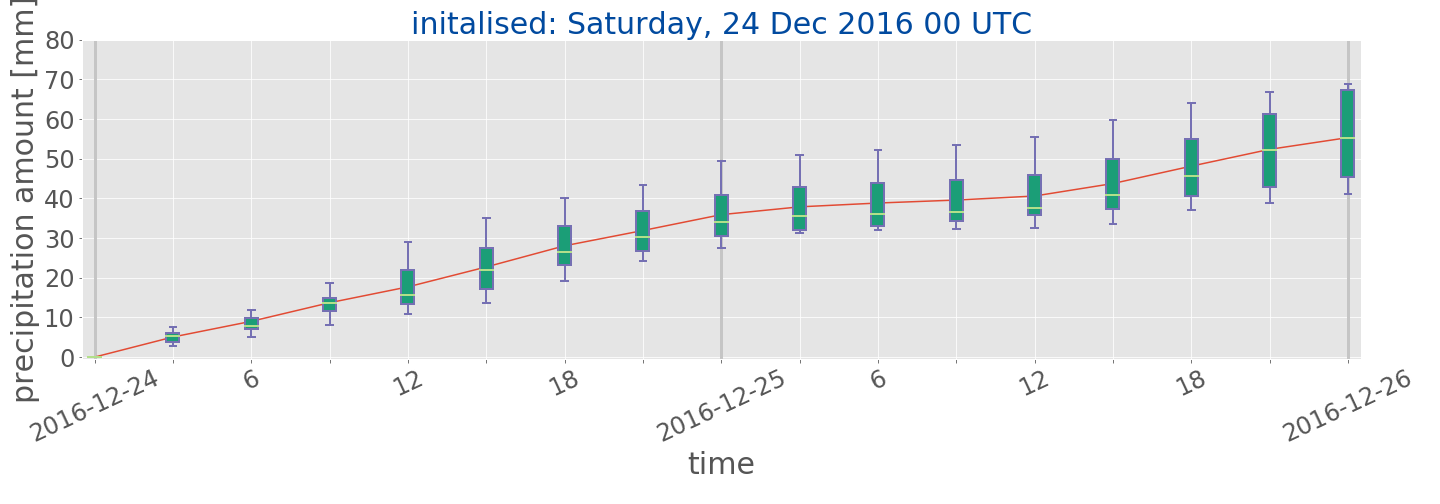
\includegraphics[trim ={0cm 2.2cm 0cm 0cm},clip,width=\textwidth]{./fig_boxplot_sfc/20161224_0}
		\caption{}\label{fig:boxplot:24}
	\end{subfigure}
	%
	\begin{subfigure}[b]{\textwidth}
		\centering
		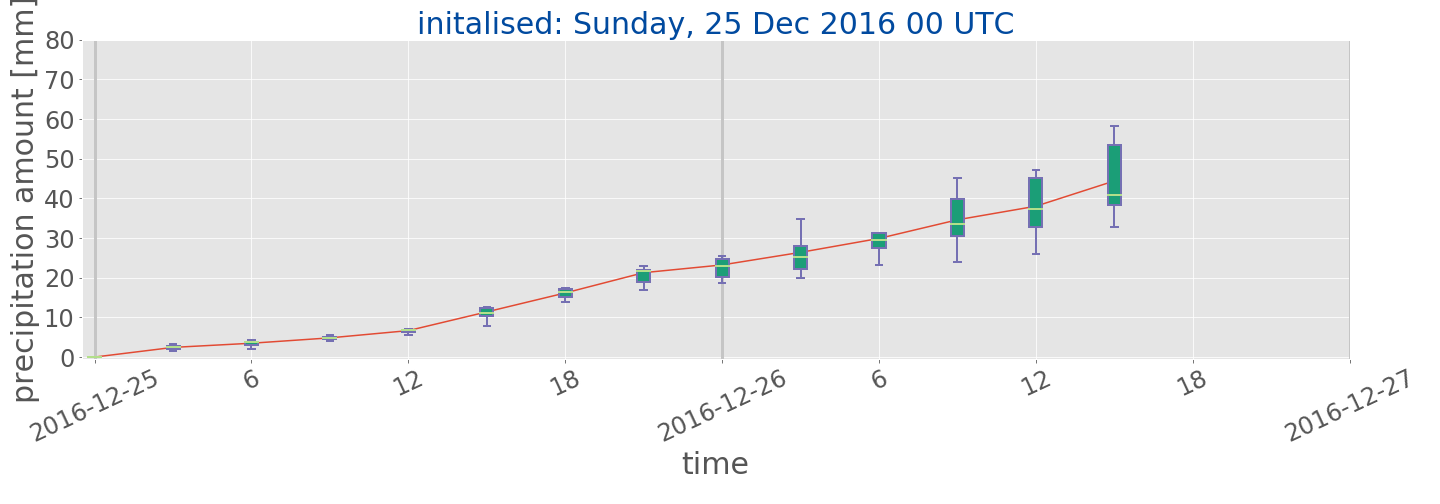
\includegraphics[trim ={0cm 2.2cm 0cm 0cm},clip,width=\textwidth]{./fig_boxplot_sfc/20161225_0}
		\caption{}\label{fig:boxplot:25}
	\end{subfigure}
	%
	\begin{subfigure}[b]{\textwidth}
		\centering
		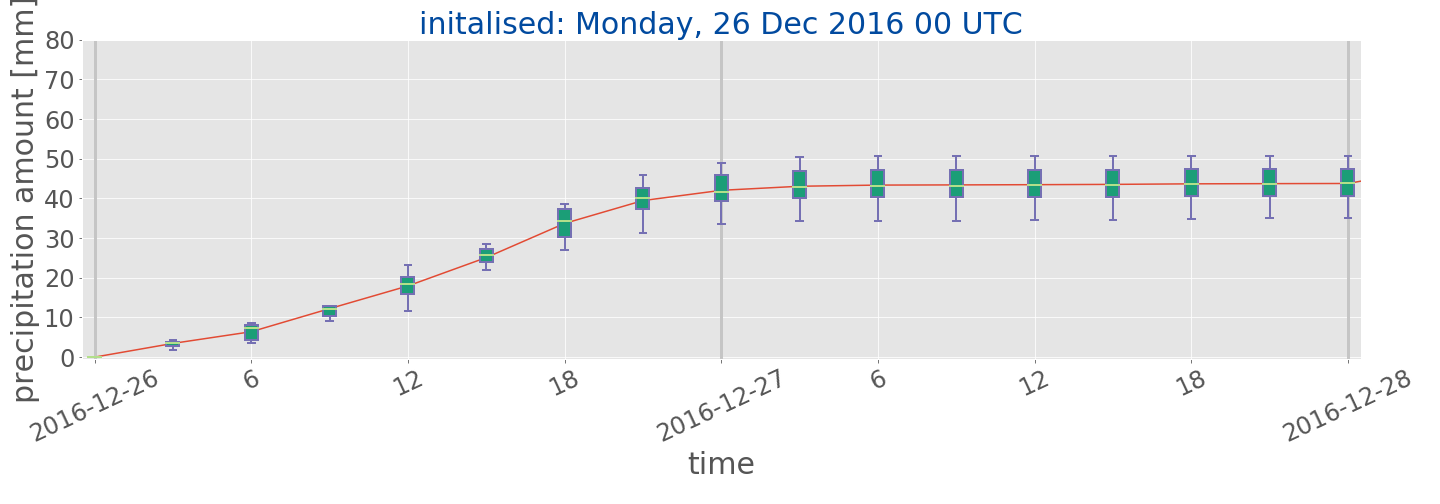
\includegraphics[trim ={0cm 1.cm 0cm 0cm},clip,width=\textwidth]{./fig_boxplot_sfc/20161226_0}
		\caption{}\label{fig:boxplot:26}
	\end{subfigure}
	\caption{Box-whisker-plot in order to quantify the statistical uncertainty of the ten ensemble members of MEPS. The red line shows the ensemble mean of all ten members and if the distribution is skewed. The short light green, horizontal line is showing the median, the wide vertical box represent the 25th and 75th percentiles, and minimum and maximum values are indicated by the vertical lines, whiskers.}\label{fig:boxplot}
\end{figure}
%%%%%%%%%%%%%%%%%%%%%%%%%%%%%%%%%%%%%%%%%%%%%%%%%%%%%%%%%%%%%%%%%%%%%%%%%%
\noindent
%%%% variability %%%%%%%%
In order to quantify the statistical uncertainty of the ensemble members, a box-whisker plot is provided in \Cref{fig:boxplot}. The box-whisker-plots in \Cref{fig:boxplot} show the time evolution of the distribution of the precipitation amount made of ten ensemble members up to \SI{48}{\hour} on \num{24}, \num{25}, and \SI{26}{\dec} (\Cref{fig:boxplot:24,fig:boxplot:25,fig:boxplot:26}). 
%The box-whisker-plot in \Cref{fig:boxplot} displays the distribution of the ten ensemble members for the respective days. 
\Cref{fig:boxplot} provides information every \SI{3}{\hour}, since some ensemble member do not have forecast values every hour.
\\
All three days with overestimation seem to have different variability between the ensemble member. As expected the forecast uncertainty increases  with longer forecast time for precipitation amount. \Cref{fig:boxplot:25} and \subref{fig:boxplot:26} show a smaller ensemble member variability on \num{25} and \SI{26}{\dec} than on \SI{24}{\dec}.
%Whereas the spread between the ensemble members is large in the beginning of \SI{24}{\dec}, the variability between the members is narrow for \num{25} and \SI{26}{\dec} for the first \SI{6}{\hour} (\Cref{fig:boxplot}). 
%More variation between the ensemble members is shown on \num{24} and \SI{26}{\dec} after \SI{3}{\hour} (\Cref{fig:ens_vari}).
% As the correlation for precipitation amount in \Cref{fig:scat:precip2426} suggests, the overestimation is not as high as for \num{24} and \SI{26}{\dec}. 
\\
%%% 24/12
Large variability is already present after \SI{3}{\hour} prediction time in \Cref{fig:boxplot:24} on \SI{24}{\dec}. The spread between the ensemble members (shown by the minimum and maximum whiskers) seems to be wide indicating a large uncertainty of the amount of surface accumulation. The ensemble mean (red line) is always higher than the median, suggesting a positively skewed distribution. 
This means more low surface precipitation amount is predicted than large surface precipitation amount at the surface.
\\
After \SI{12}{\hour} forecast time, the median is closer to the lower 25th percentile, indicating a negative skewness. Also, all upper whiskers in \Cref{fig:boxplot:24} are longer than the lower ones. %, which would follow that the ensemble members vary amongst the most positive quartile and that it is very similar for the least positive quartile group. 
This shows, that more ensemble members predict high precipitation amount instead of little.
\\
%%% 25/12
The variability in \Cref{fig:ens_vari} show no large variation between the ensemble members (narrow box-whiskers) on \SI{25}{\dec}. This day is also the forecast with the smallest wet bias of \SI{5}{\mm} on the three days with overestimation (\Cref{fig:bias:precip12}). This may be related to the small variability between the ensemble members in \Cref{fig:boxplot:25}. 
%As \Cref{fig:boxplot:25} shows, 
The variability in the forecast increases after \SI{15}{\hour} prediction time. %In general, m
Median and mean agree well for the entire period of a \SI{48}{\hour} lead time. After \SI{39}{\hour} the mean is much higher than the median in \Cref{fig:boxplot:25}, indicating that more surface precipitation amount is predicted by most ensemble members. %and closer to the lower 25th percentile . 
It seems, that all ten ensemble members agree well on the prediction and nevertheless MEPS overestimates the surface accumulation. 
\\
%%% 26/12
%On \SI{26}{\dec}, the box-whiskers are 
%narrower for the first \SI{30}{\hour} in \Cref{fig:boxplot:25}, but slightly larger after \SI{6}{\hour} forecast time. %for initialisations on \SI{26}{\dec}. %\Cref{sec:res:large_scale_sfc} presented a good agreement between observations and forecast of large scale features in terms of pressure, temperature, and wind direction.
On \SI{26}{\dec} the highest deviation to the double fence observations is estimated (\Cref{tab:res:MEPS_err_10}). The precipitation amount forecast is overestimating at \SI{12}{\UTC} in \Cref{fig:sfc_acc26}. \Cref{fig:boxplot:26} indicates increasing variability after \SI{6}{\hour}, but the variability between the ensemble members is not as large as on \SI{24}{\dec} after \SI{12}{\hour} lead time. Nevertheless, agree the ensemble member the least about the precipitation amount at \SI{12}{\UTC}. The spread between the ensemble members is wide showing the variability of the forecast members. As \Cref{fig:sfc_acc26} also shows is the double fence observation not within the spread of the ensemble member after \SI{9}{\hour} lead time. 
%The box-whiskers in \Cref{fig:boxplot:26} indicate more variability after \SI{6}{\hour} lead time on \SI{26}{\dec}.%prediction while 
%The forecast precipitation amount is similar to the double fence observations, but overestimated.
% %and following the structure of the double fence observation. 
% Variability of all ensemble members increases at \SI{6}{\hour} lead time, but then decreases again in \Cref{fig:boxplot:26}. 
% \\
% %Since the deterministic forecast, black line in \Cref{fig:sfc_acc24}, is in the upper percentile compared to its perturbed members it follows that for this forecast the deterministic forecast was not the best guess for the surface accumulation and by using the 'wrong' initial state it can have led to larger miscalculations. 
% \\
% %%%% DISCUSSION %%%%%
According to \citet{muller_arome-metcoop:_2017} strong precipitation events are better predicted with AROME-MetCoOp than with ECMWF. In \Cref{sec:dim:dec_obs} it was described, that during \num{21} to \SI{27}{\dec} \SI{56.9}{\percent} of the total December 2016 accumulation of precipitation were observed. The extreme 2016 Christmas event follows to be a strong precipitation event. 
%%% 10 % double fence
%Furthermore could it be related to the \SI{10}{\percent} under-catchment by the double fence gauge under high wind condition.
The overestimation at the surface could be related to the \SI{10}{\percent} under-catchment by the double fence gauge under high wind condition. As \Cref{tab:res:MEPS_err_10} indicates the difference between the forecast system and the double fence observations is decreased, but still too much surface accumulation is estimated by MEPS. The difference for \SI{12}{\hour} lead time on \num{25} and \SI{26}{\dec} is however more than \SI{40}{\percent}. Only a \SI{10}{\percent} under-catchment by the double fence is assumed in this thesis. 
%This value is approximated by \citet{wolff_wmo_2018}, [unpublished] from measurement sites for wind speed below \SI{9}{\mPs}. 
\citet{wolff_wmo_2018}, [unpublished] states that estimates for higher wind speeds such observed at Haukeliseter do not exist but is hypothesized to be within \SI{20}{\percent}. During the event the \SI{10}{\metre} observed wind was less than \SI{20}{\mPs} for \SI{10}{\minute} averaged wind speeds prior the full hour.
The forecast error could be reduced because of the wind related effect of the double fence.
\\
\\
%%% synoptic
The uncertainty of the surface accumulation might also have been related to the fact that the large-scale situation intensified more than low pressure systems in Norway usually do. 
\\
%%% 24/12
The overestimation on \SI{24}{\dec} can be related to the high precipitation amount in the evening of \SI{23}{\dec}.
The precipitation amount associated with the transition of the occluded front on \SI{23}{\dec}, after \SI{18}{\UTC}, is higher than on previous days (\Cref{fig:sfc_acc23} and \Cref{fig:TPU23}). During \num{20} to \SI{21}{\dec}, the hourly precipitation around \SI{0}{\UTC} is less intense than on \SI{23}{\dec} (\Cref{fig:TPU23}). High accumulation amount over shorter time followed and could have resulted in a larger variability of the MEPS members (\Cref{fig:boxplot}). 
In the analysis cycle \SI{3}{\hour} prior the initialisation of MEPS observations are included inside the model domain \citep{homleid_verification_2016}. Since the precipitation amount associated with the occlusion passage on \SI{23}{\dec} was quite high, might this have led to the overestimation of surface precipitation amount. \citep{homleid_verification_2016}
\\
Another possibility is that MEPS might have accounted for more precipitation  around \SI{12}{\UTC} on \SI{24}{\dec} than was observed. This could show the large predicted precipitation amount in \Cref{fig:sfc_acc24} at \SI{13}{\UTC}.
\\
%%% 25/12
On \SI{25}{\dec} MEPS surface forecasts suggest that MEPS did not expect the occurrence of a warm front (\Cref{fig:res:sfc_pres25,fig:res:sfc_temp25,fig:res:sfc_wd25,fig:res:sfc_ws25}). 
However, from the surface accumulation prediction 
%could suggest 
it could be concluded that MEPS expected more precipitation around \SI{12}{\UTC} on \SI{25}{\dec}. Maybe MEPS has expected a less intense warm-front passage and therefore more precipitation. The fact that the temperature is rising and therefore the phase is changing from snow to liquid precipitation (\Cref{fig:res:obs_masc}) may have led to MEPS expecting more liquid precipitation% rather than mixed phase precipitation and 
hence MEPS predicted more surface accumulation.
%I consider that MEPS misinterpreted the amount of precipitation related to the transition of the warm sector.  
\\
%%% 26/12
On \SI{26}{\dec} between \SIlist{15;18}{\UTC}, the core of the Christmas 2016 low-pressure system passes over Haukeliseter (\Cref{fig:res:sfc_pres26,fig:res:sfc_temp26,fig:res:sfc_wd26,fig:res:sfc_ws26}). Overestimation of surface accumulation are seen after \SI{12}{\UTC} in \Cref{fig:sfc_acc26}. It is very likely that overestimation on \SI{26}{\dec} is related to passage of the low pressure system, since ensemble prediction systems are not adjusted to predict perfectly for extreme events.
\\
\\
%%% spin-up
% I assume that the uncertainty appearing already after \SI{3}{\hour} on \SI{24}{\dec} (\Cref{fig:boxplot:24}) could be associated with a longer spin-up time of MEPS than general. MEPS usually has a spin-up time of about six hours \citep{Priv_Comm_Koltzow}. 
Observations are used as initial condition in weather forecast systems, such as MEPS.
As described in \Cref{sec:DIM:MEPS}, should the observations be within the spread of the ensemble member prediction. Furthermore, the forecast members should be close together for a short time, so they may be considered \textit{deterministic}. 
%. which are going to be used for the initialisation are within the 
This is not the case for \num{24} to \SI{26}{\dec} after \SI{12}{\hour} lead time.
\\
Uncertainties appearing already after \SIlist{3;6}{\hour} on \num{24} and \SI{26}{\dec} could be associated with a long spin-up time of MEPS. As described in \Cref{sec:DIM:MEPS}, MEPS precipitation has a spin-up time of \SI{6}{\hour} and values before that should not be used as very certain \citep[][personal communication]{Priv_Comm_Koltzow}. Even though this is taken into account, \Cref{fig:boxplot} show larger variability for the ensemble members on \num{24} and \SI{26}{\dec} after \SI{6}{\hour} prediction.
\\
As a result of poorer initial conditions the spin-up time could have been longer on \num{24}, \num{25}, and \SI{26}{\dec}. The spin-up time can vary due to less or also uncertain observations going into the initialisation \citep{warner_tutorial_1997}. 
Observations are fed into MEPS directly by using the operational global forecast model ECMWF. %, which initialises observations. 
Less observations can be due to instrumentation failure or the data has not been transmitted in time to the forecasting system. Observations and data assimilation have errors and this can increase the initial uncertainty in a weather forecast. 
Boundary conditions have also uncertainties, such as insufficient details of the sub-grid scale and parametrised surface fluxes \citep{owens_ecmwf_2018}. 
The atmosphere is a chaotic system and it depends sensitive on initial conditions. Small uncertainties can to large errors \citep{lorenz_atmospheric_1969}. Furthermore, model uncertainties such as parametrisations of physical processes and the limited model resolution exist. Because of these errors the model needs to stabilise. When the stabilised state is reached the results can be more trusted \citep{Hollingsworth_experiment_79}.
%Furthermore, the deterministic and perturbed members might not to have reached a stable state yet and show larger variation in \Cref{fig:boxplot:24} and \subref{fig:boxplot:26} from early on than e.g. on \SI{25}{\dec}. 
Longer spin-up time than the usually \SI{6}{\hour} for precipitation can lead to larger variation from early on in \Cref{fig:boxplot:24} and \subref{fig:boxplot:26} 
%from early on 
than e.g. on \SI{25}{\dec}.
More variability between the ensemble members does not necessarily mean that a forecast is bad, it only shows the predictability. %uncertainty of the initial conditions. 
\\
Since the box-whisker-plot in \Cref{fig:boxplot:25} (\SI{25}{\dec}) show less variability in the beginning it is assumed that spin-up time issues are less likely, but not totally excluded. It could be related to an error in the initialisation, even though it does not show within the variability at the beginning.
%Important is, 
%As described in \Cref{sec:DIM:MEPS} the perturbed members should always lie relatively close to the observations. This means that they should be almost similar as the deterministic for a short time In mesoscale prediction should the forecast member be close together for a short time. 
%\\
%It seems, that the initial and boundary conditions for MEPS might have not been perfect for initialisations on \SI{24}{\dec} at \SI{0}{\UTC}. 
%Observations are fed into MEPS indirectly by using the operational global forecast model ECMWF, which initialises observations. 
% The regional model MEPS receives initial and boundary conditions from ECMWF for its model set up \citep{muller_arome-metcoop:_2017}.
% The initial conditions such as observations and the model itself have uncertainties.
% %An error associated with the spin-up time of MEPS is not totally excluded for these days. 
% In \Cref{fig:sfc_acc25} and \subref{fig:sfc_acc26}, the ensemble mean agrees well with the deterministic forecast, which is an indication of a symmetrical spread around the deterministic run. Again, the ensemble mean is the best statistical solution over a longer timespan and does not necessarily mean to be the best for an extreme event such as the Christmas storm 2016. 
\\
\\
%%% topography
% The overestimation of surface accumulation could be associated to the local horizontal resolution effect of MEPS at Haukeliseter, which will be further discussed in \Cref{sec:res:oro_infl}. 
The overestimation of accumulated precipitation during \num{24} and \SI{26}{\dec} might be related to
% %to the high forecasted wind speeds, 
local horizontal resolution of MEPS at Haukeliseter as well as to the complex development of the low-pressure system north-west of Norway on \SI{24}{\dec}. 
\\
%Generally, ensemble prediction forecast systems are overall performing best during usual large-scale weather situations. 
Ensemble prediction systems have the advantage that they present the variability of possible observation. % and not to present extreme events particularly well. Still, t
%Observations should be within the spread of the ensemble members. The ensemble presenting possibilities .
The studies from \citet{petroliagis_potential_1997,buizza_probabilistic_1999} show that the ECMWF ensemble prediction can be extremely beneficial for evaluating the forecast skill during extreme precipitation events. The spread between the ensemble members should include the uncertainty of surface observation. This might not always be the case, especially during extreme events, if high amounts of precipitation are expected over a short time. 
\\
%Therefore, i
%It is more 
Another likelihood for the simulation of high precipitation amount during the intensification of the extreme event may be related to the local topography and the strong winds. Furthermore, the orographic representation in the regional model MEPS can influence the simulation. Effects of the topographical resolution on MEPS at Haukeliseter, will be further discussed in \Cref{sec:res:oro_infl}. 
\\
Even though with the launch of MEPS the variation of observations is covered, the forecast system seems not to be able to represent surface precipitation amount for this particular extreme weather event. 
% \\
% \\
% \textcolor{red}{MOVE TO VARI PLOT}
% \Cref{fig:boxplot:25} and \subref{fig:boxplot:26} show a smaller ensemble member variability on \SIlist{25;26}{\dec} than on \SI{24}{\dec}. 
% While the occlusion on \SI{26}{\dec} is apparent (\Cref{fig:res:sfc_pres26,fig:res:sfc_temp26,fig:res:sfc_wd26,fig:res:sfc_ws26}), the warm front development on \SI{25}{\dec} is less obvious (\Cref{fig:res:sfc_pres25}, \subref{fig:res:sfc_temp25}, \subref{fig:res:sfc_wd25}, \subref{fig:res:sfc_ws25}). 
% \\
% On \SI{25}{\dec} the overestimation started to occur around \SI{13}{\UTC} in \Cref{fig:sfc_acc25}, and may be related to the delayed temperature MEPS forecasted temperature increase in \Cref{fig:res:sfc_temp25}.  
% \\
% %\citet{muller_arome-metcoop:_2017} states also, that an overestimation appears, where the precipitation event (\SI{12}{\hour} accumulation) is less than \SI{10}{\mm} this seems not to be true for all days but could be possible for \num{25} and \SI{26}{\dec} (observed accumulation in \Cref{tab:sfc_acc}). 
% In December 2014, the \SI{12}{\hour} precipitation mean absolute error in AROME-MetCoOp was below \SI{1.5}{\mm} \citep{muller_arome-metcoop:_2017}. For the 2016 Christmas storm the mean absolute error is less than \SI{7}{\mm} for \SI{12}{\hour} of accumulation on \SI{25}{\dec}
% (\Cref{fig:MAE:precip12}), but reaches up to \SI{15}{\mm} on \num{24} and \SI{26}{\dec}. 
% %Therefore, the assumption follows that on \SI{26}{\dec} the overestimation might be correlated to the <\SI{10}{\mm} problem described by \citet{muller_arome-metcoop:_2017}. 
% The \SIlist{12;24}{\hour} accumulation is presented in \Cref{tab:res:MEPS_err} for Haukeliseter and shows that \SI{12}{\hour} observed accretion was less than \SI{10}{\mm} for 
% \num{25} and \SI{26}{\dec}.
% %On \SI{25}{\dec} the mean absolute error was \SI{1.1}{\mm} for the first \SI{12}{\hour} accumulation and shows that this could be an influence but does not necessarily mean to be the case, because the general mean absolute error is small (\Cref{fig:MAE:precip}). 
% The mean error for \SI{12}{\hour} accumulation in fact shows a wet bias during \num{24} and \SI{26}{\dec}.
% %since the overestimation started to occur after \SI{11}{\hour} prediction time. 
% %%%%%%%%%%%%%%%%%%%%%%%%%%%%%%%%%%%%%%%%%%%%%%%%%%%%%%%%%%%%%%%%%%%%%%%%%%


%%%%%%%% large scale phenomena vertical ? %%%%%%%%%%%%%%
\subsection{Vertical Comparison of Snow Water Content}
\label{sec:res:large_scale_vert}
Frontal passages were observed at the surface several times throughout the extreme storm in December 2016. MEPS is able to predict the large scale synoptics and related precipitation, temperature, and wind changes for initialisation more than \SI{24}{\hour} in advance (\Cref{sec:res:large_scale_sfc}). Three additional instruments were installed %to measure the vertical snow water content 
to measure frozen precipitation up to \SI{3}{\km} at Haukeliseter. 
%%%%%%%%% image reflectivity %%%%%%%%%%%%%%
\begin{figure}[H]
	\centering
	% 23/12
	\begin{subfigure}[t]{\textwidth}
		\centering
		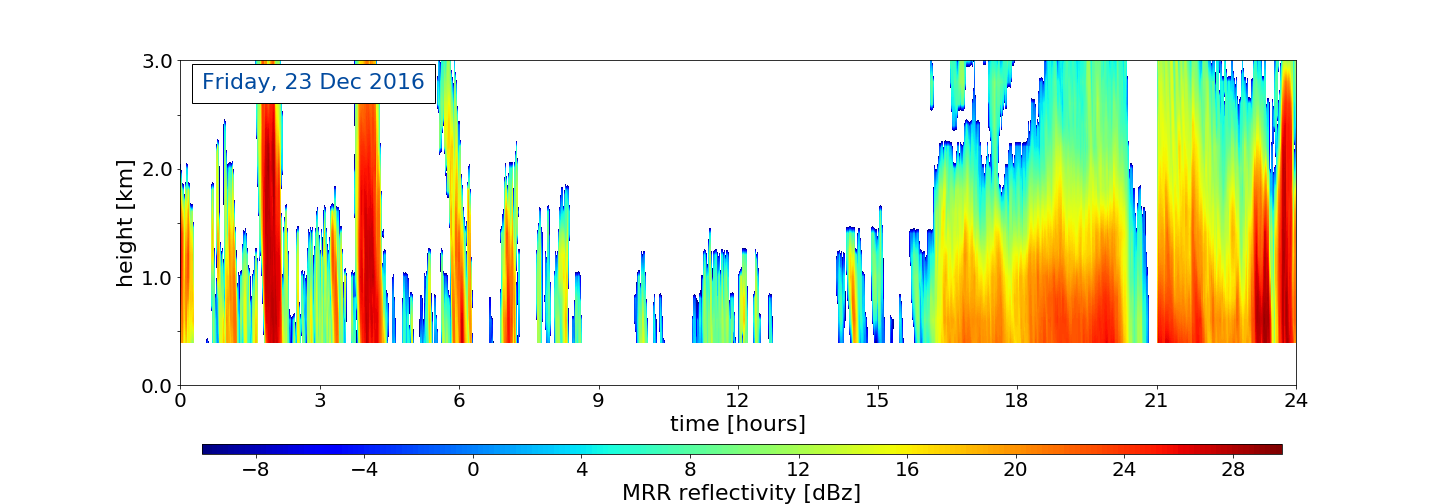
\includegraphics[trim={4.cm 2.5cm 4.5cm 1.5cm},clip,width=0.91\textwidth]{./fig_MRR_refl/MRR_20161223}
		\caption{}\label{fig:ret:refl23}
	\end{subfigure}
	% 24/12
	\begin{subfigure}[t]{\textwidth}
		\centering
		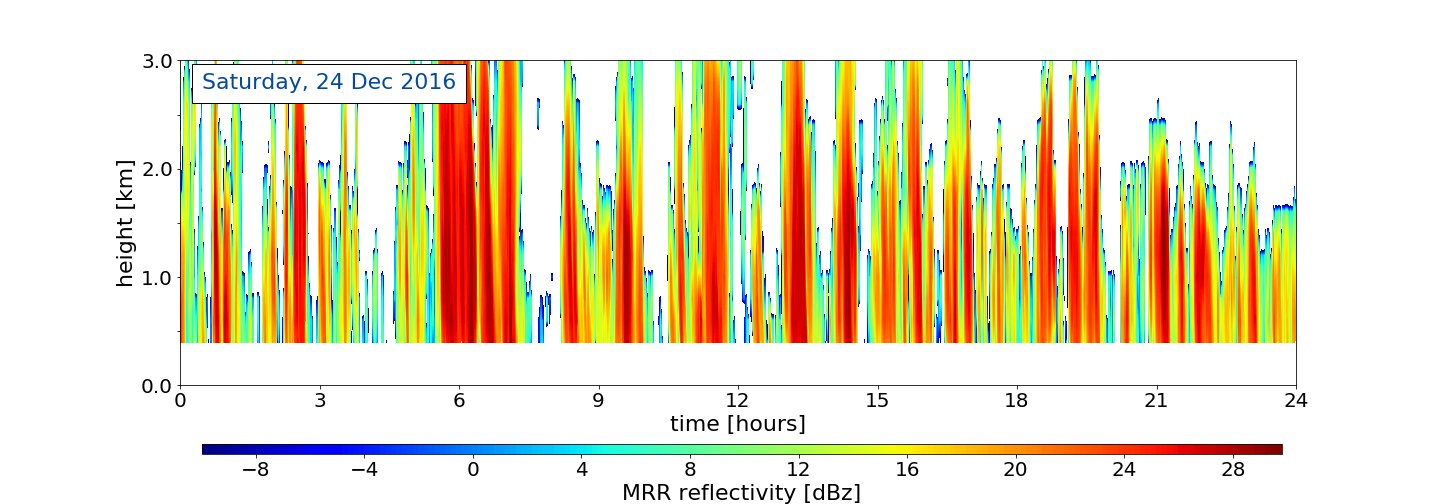
\includegraphics[trim={4.cm 2.5cm 4.5cm 1.5cm},clip,width=0.91\textwidth]{./fig_MRR_refl/MRR_20161224}
		\caption{}\label{fig:ret:refl24}
	\end{subfigure}
	% 25/12
	\begin{subfigure}[t]{\textwidth}
		\centering
		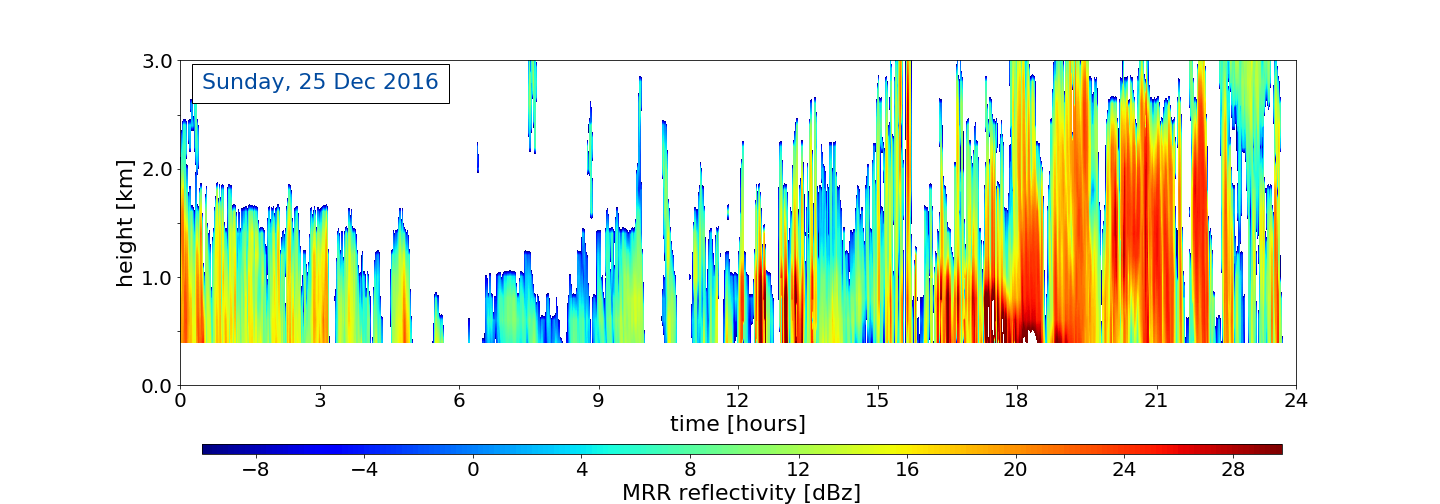
\includegraphics[trim={4.cm 2.5cm 4.5cm 1.5cm},clip,width=0.91\textwidth]{./fig_MRR_refl/MRR_20161225}
		\caption{}\label{fig:ret:refl25}
	\end{subfigure}
	% 26/12
	\begin{subfigure}[t]{\textwidth}
		\centering
		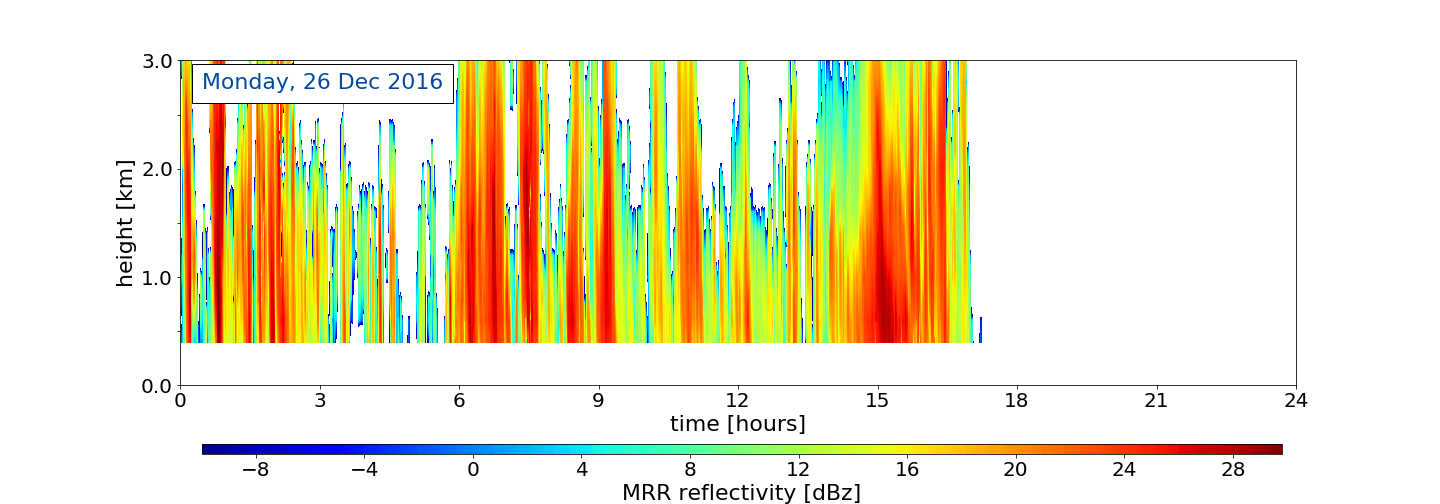
\includegraphics[trim={4.cm 2.5cm 4.5cm 1.5cm},clip,width=0.91\textwidth]{./fig_MRR_refl/MRR_20161226}
		\caption{}\label{fig:ret:refl26}
	\end{subfigure}
	% label
	\begin{subfigure}[t]{\textwidth}
		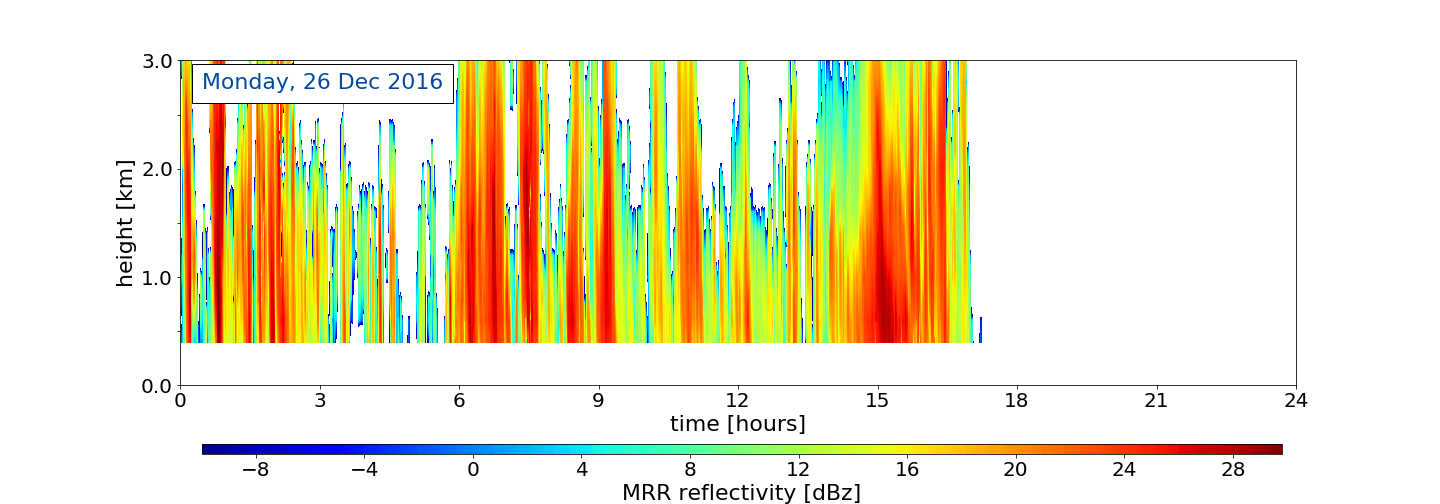
\includegraphics[trim={6.5cm 0cm 5.3cm 15.5cm},clip,width=\textwidth]{./fig_MRR_refl/MRR_20161226}
	\end{subfigure}
	\caption{MRR reflectivity for the days with frontal passage and overestimation at the ground at Haukeliseter. \SI{}{\decibel Z} reflectivity according to the colour bar, with weaker precipitation in blue and more intense precipitation in red. Presenting the reflectivity without applying the environmental masks described in \Cref{sec:pre_snow}. \protect\subref{fig:ret:refl23}--\protect\subref{fig:ret:refl26} \num{23} to \SI{26}{\dec}.}\label{fig:ret:refl}
\end{figure}
%%%%%%%%%%%%%%%%%%%%%%%%%%%%%%%%%%%%%%%%%%%%%%%%%%%%%%%%%%%%%%%%%%%%%%%%%
\noindent
This %unique approach 
gives the opportunity to compare the forecasts %of SWC with frozen precipitation observations in the vertical. 
with retrieved vertical snow water content (\Cref{sec:ret:sensitivity,sec:ret_dofe_comp}).
This study is unique because it uses state of the art vertical measurement to compare to an ensemble prediction forecast system. As far as the author is aware of there is no study about verification of MEPS for the vertical %ensemble member prediction models 
with observations.
\\
The motivation to compare regional model forecasts with vertical snow measurements resulted from a study by \citet{joos_influence_2012}. They did sensitivity studies on the microphysical scheme of COSMO (COnsortium for Small-scale MOdelling) and found that the storm development depends on the correct vertical placement of the precipitation inside a modeled storm. Vertical precipitation placement determines the vertical profile of latent heating, and hence the generation of potential vorticity which in return shows if a storm strengthens or weakens. Correct vertical precipitation observations can then help to correctly evaluate model vertical precipitation patterns.
%Previous studies such as \citet{joos_influence_2012} motivate to make accurate surface measurements more available to improve mesoscale models.
\\
Passages of occluded fronts and a warm sector were observed on \num{23}, \num{26}, and \SI{25}{\dec}. Additionally, an overestimation at the ground is shown on  \num{24}, \num{25}, and \SI{26}{\dec} for surface precipitation amount (\Cref{sec:sfc_acc}, \Cref{fig:sfc_acc}). 
\\
\\
\Cref{fig:ret:refl} shows the reflectivity from the MRR at Haukeliseter for these days. Likely periods of frozen precipitation are inidcate with orange and red in \Cref{fig:ret:refl}.% areas with orange and red indicate likely periods with snowfall. 
On \SI{26}{\dec} only values until \SI{17}{\UTC} are displayed, because of the temperature change and hence a precipitation shift led to liquid drops freezing on the MRR dish so that the signal got attenuated.
\\
During the Christmas 2016 extreme event two precipitation patterns are seen in the vertical. First, a continuous precipitation pattern with constant precipitation over several hours. In the following it is referred to as \textit{continuous}.
The second pattern shows interchangeable high and low amounts of snow over \SI{1}{\hour}. This will be referred to as \textit{pulsing}.
\\
\\
%%%% fronts upslope (23+26) %%%%
More continuous precipitation pattern with high reflectivity values in \Cref{fig:ret:refl} indicate the transition of the occlusion on \num{23}, \num{26}, and the warm sector passage on \SI{25}{\dec}.
The high reflectivity on \num{23} and \SI{26}{\dec} shows the passage of the occlusion and the associated frozen precipitation.
\\
% 23/12
On \SI{23}{\dec}, the surface observations of sea level pressure (\Cref{fig:res:sfc_pres23}), \SI{2}{\metre} air temperature (\subref{fig:res:sfc_temp23}), and \SI{10}{\metre} wind (\subref{fig:res:sfc_wd23}), allow to assume that the occluded front passed through Haukeliseter between \SIlist{12;21}{\UTC}.
\Cref{fig:ret:refl23} shows high observed reflectivity in the lower up to \SI{3}{\km} at Haukeliseter after \SI{16}{\UTC}.
%The observation of the lower atmosphere at Haukeliseter show high reflectivity and therefore more intense precipitation after \SI{16}{\UTC} (). 
After \SI{16}{\UTC}, the wind is from the south, upslope (\Cref{fig:res:sfc_wd23}, \Cref{fig:site:kartverket}) which led to a continuous precipitation pattern in \Cref{fig:ret:refl23}. 
In the morning of \SI{23}{\dec} high amount of frozen precipitation was observed at \SIlist{2;4}{\UTC}, but with a more pulsing pattern than in the evening.
\\
% 26/12
Another occlusion passed through on \SI{26}{\dec} between \SIlist{15;21}{\UTC} (compare surface observations \Cref{fig:res:sfc_pres26} to \subref{fig:res:sfc_precip26}). A pulsing precipitation pattern and high reflectivity in \Cref{fig:ret:refl26} indicate the passage after \SI{15}{\UTC}. 
%%%% warm sector --> liquid (25) %%%%%
While on \num{23}, \num{24}, and \SI{26}{\dec} the reflectivity did not pass values larger than \SI{28}{\decibel Z}, \Cref{fig:ret:refl25} shows high reflectivity values larger than \SI{30}{\decibel Z} on \SI{25}{\dec} (compare for approximation \Cref{tab:ref_values}). 
These high reflectivity values up to \SI{1.2}{\km} in \Cref{fig:ret:refl25} indicate the observation of possible liquid precipitation on \SI{25}{\dec}. Images from the MASC were able to verify observed liquid drops during \SIrange{12}{21}{\UTC} (\Cref{fig:res:obs_masc}). 
In the observations on \SI{25}{\dec}, %patterns of possible liquid precipitation (\Cref{fig:res:obs_masc}) related to 
high temperatures (\Cref{fig:res:sfc_temp25}) %and high reflectivity (\Cref{fig:ret:refl25}) 
are shown, between \SIrange{12}{21}{\UTC}. %High reflectivity is present around \SI{18}{\UTC} with layer thickness up to \SI{1.2}{\km} (\Cref{fig:ret:refl25}).
%%%% turbulent (24+26) %%%%%
% 24/12
On \SI{24}{\dec} short, interchangeable high and low reflectivity patterns are present in \Cref{fig:ret:refl24}. \Cref{fig:res:sfc_wd24} and \subref{fig:res:sfc_ws24} indicate strong wind from the west which led to a pulsing precipitation structure in \Cref{fig:ret:refl24} on \SI{24}{\dec}. 
% 26/12
The same pulsing is seen on \SI{26}{\dec} before \SI{12}{\UTC} in \Cref{fig:ret:refl26}. A comparison with the observed surface wind in \Cref{fig:res:sfc_wd26} and \subref{fig:res:sfc_ws26} shows also westerlies.  The orographic influences on the surface wind and therefore a possible relation to the precipitation patterns will be further investigated in \Cref{sec:res:oro_infl}. 
% %The transit of the boundaries is shown in \Cref{fig:ret:refl} by more consistent structure of a storm with higher reflectivity values. 
\\
\\
%%%% SWC %%%%%%%%%
%%%%%%%%% image SWC retrieval MEPS 21 %%%%%%%%%%%%%%
\begin{figure}[H]
	\centering
	% 23/12
	\begin{subfigure}[t]{1.05\textwidth}
		\centering
		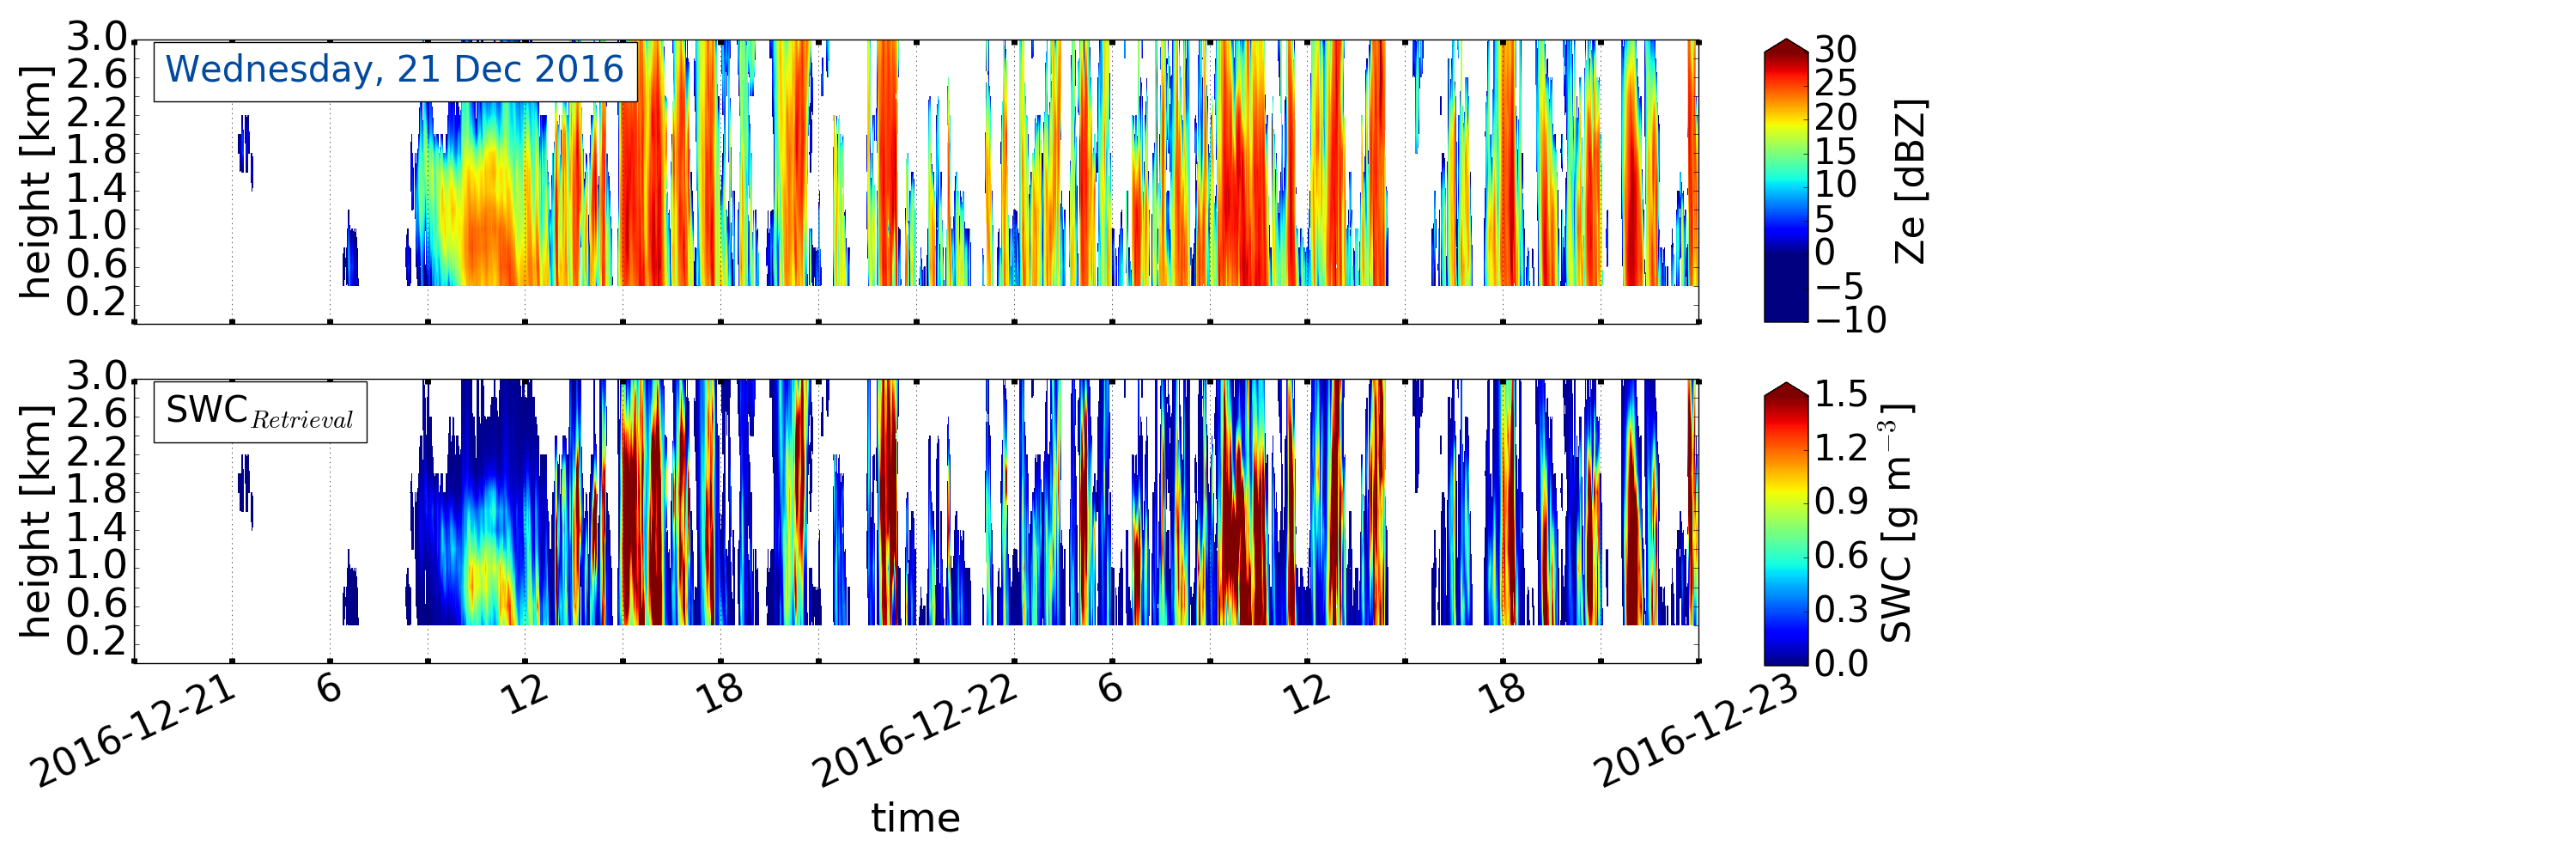
\includegraphics[trim={0.cm 2.2cm 19.cm 0.5cm},clip,width=0.9\textwidth]{./fig_obs_ret/20161221}
		\caption{}\label{fig:SWC:ret_21}
	\end{subfigure}
	% EM
	\begin{subfigure}[t]{1.05\textwidth}
		\centering
		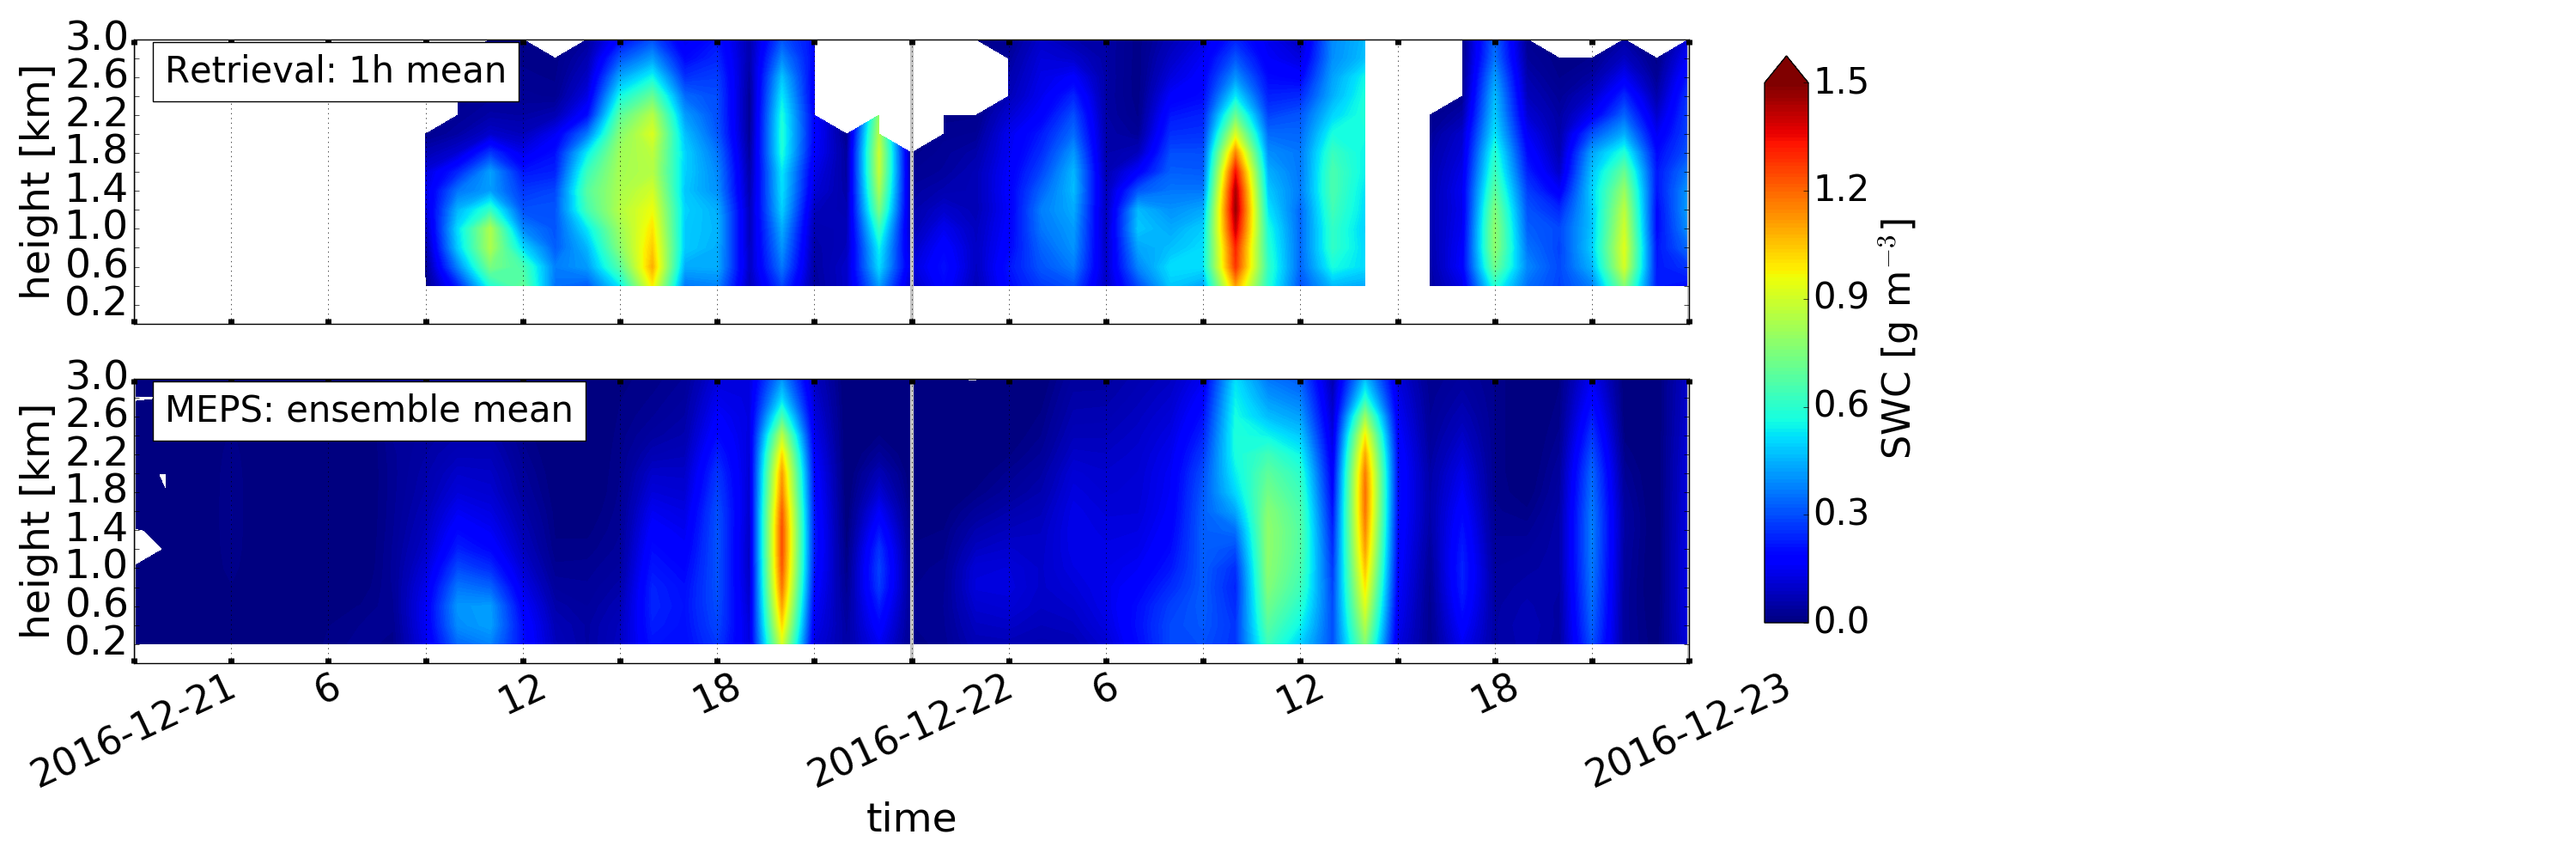
\includegraphics[trim={0.cm 2.2cm 19.cm 0.5cm},clip,width=0.9\textwidth]{./fig_vert_SWC_EM/20161221}
		\caption{}\label{fig:SWC_EM:21}
	\end{subfigure}
	% 3h
	\begin{subfigure}[t]{1.05\textwidth}
		\centering
		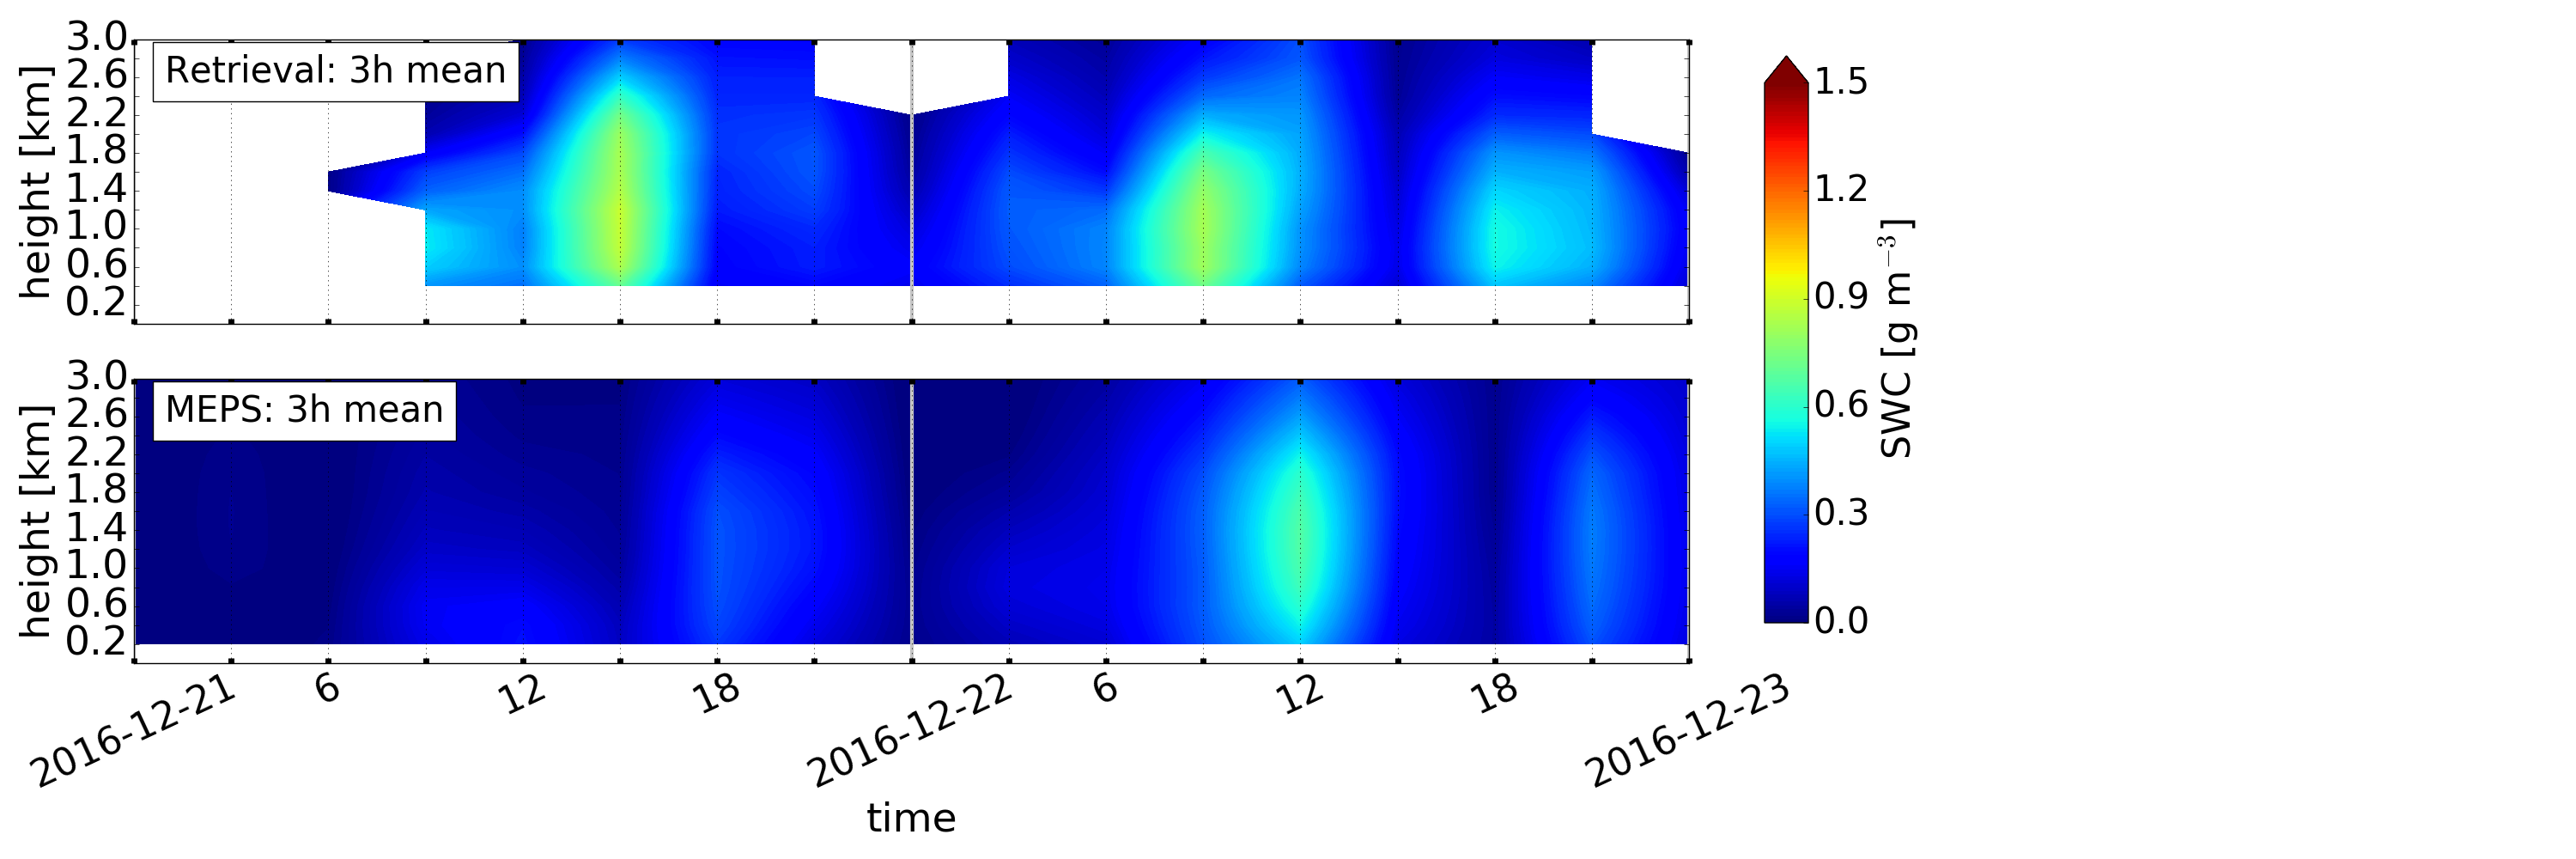
\includegraphics[trim={0.cm 0.8cm 19.cm 0.5cm},clip,width=0.9\textwidth]{./fig_vert_SWC_3h/20161221}
		\caption{}\label{fig:SWC3h:21}
	\end{subfigure}
	\caption{Initialisation on \SI{21}{\dec} at \SI{0}{\UTC}. From top to bottom: (\protect\subref{fig:SWC:ret_21}) MRR reflectivity for \SI{48}{\hour}, minutely retrieved snow water content.
		(\protect\subref{fig:SWC_EM:21}) Hourly averaged retrieved snow water content, lower panel instantaneous hourly ensemble mean, % averaged forecast of all ensemble member SWC, 
        neglecting missing values. 
		(\protect\subref{fig:SWC3h:21}) Three hourly averaged retrieved snow water content, lower panel instantaneous three hourly ensemble mean. %averaged forecast of all ensemble member SWC.
        }\label{fig:SWC21}
\end{figure}
%%%%%%%%%%%%%%%%%%%%%%%%%%%%%%%%%%%%%%%%%%%%%%
%%%%%%%%% image SWC retrieval MEPS 22 %%%%%%%%%%%%%%
\begin{figure}[H]
	\centering
	% 23/12
	\begin{subfigure}[t]{1.05\textwidth}
		\centering
		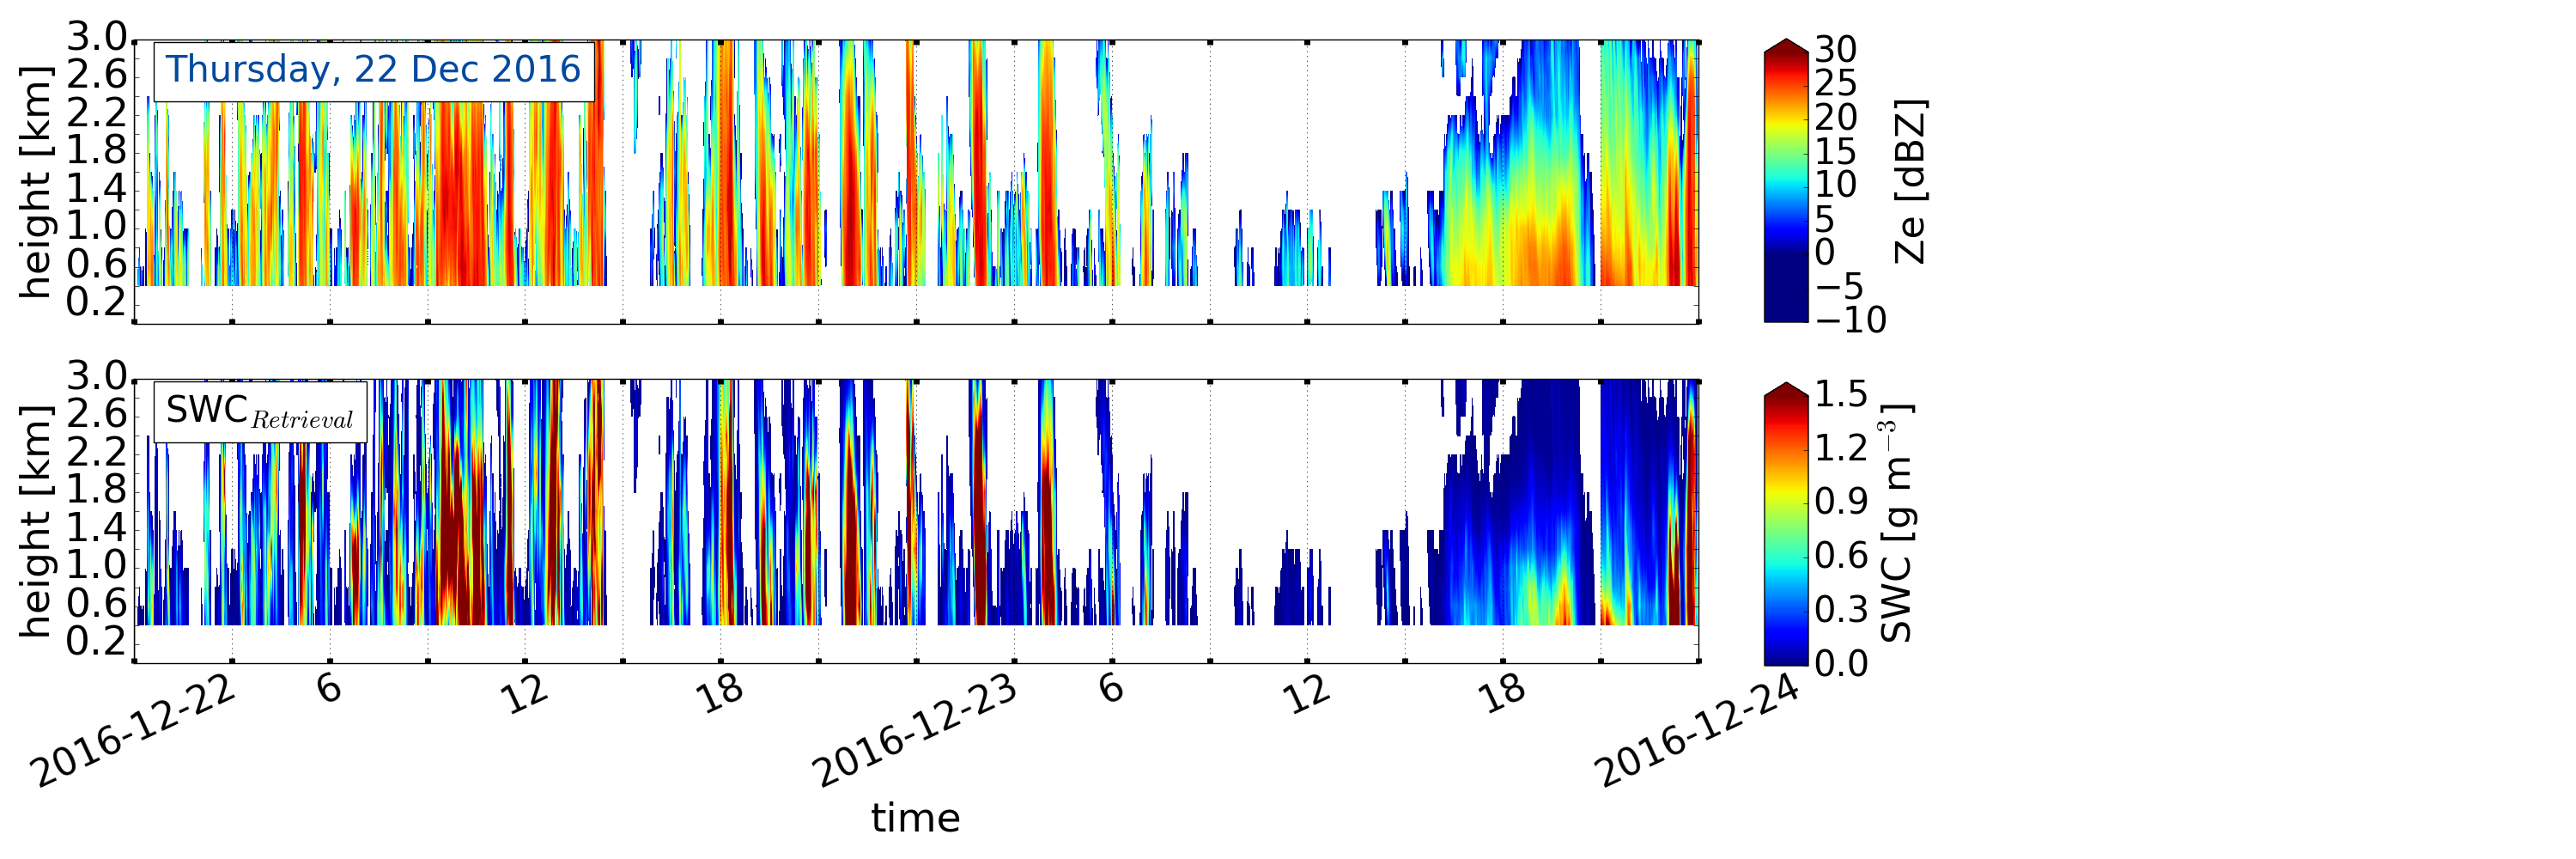
\includegraphics[trim={0.cm 2.2cm 19.cm 0.5cm},clip,width=0.9\textwidth]{./fig_obs_ret/20161222}
		\caption{}\label{fig:SWC:ret_22}
	\end{subfigure}
	% EM
	\begin{subfigure}[t]{1.05\textwidth}
		\centering
		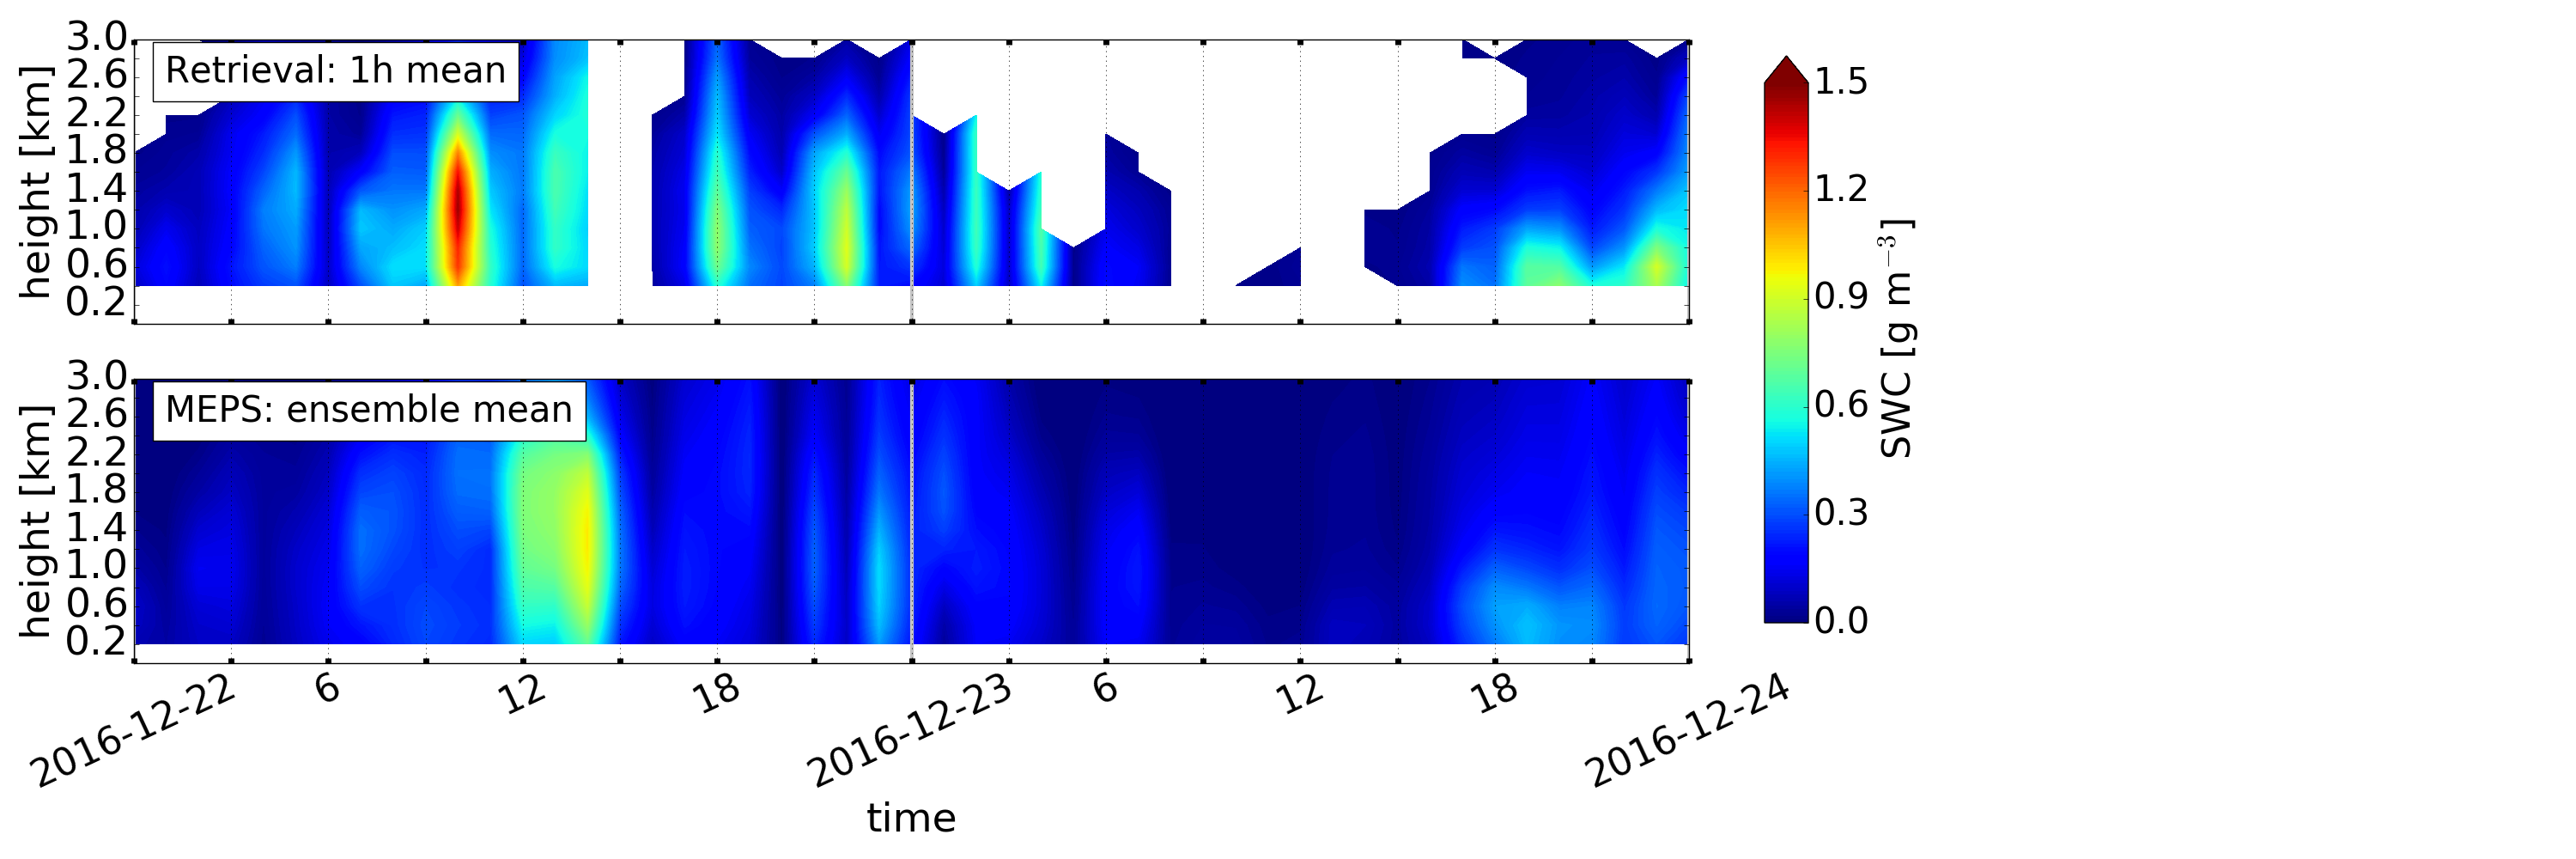
\includegraphics[trim={0.cm 2.2cm 19.cm 0.5cm},clip,width=0.9\textwidth]{./fig_vert_SWC_EM/20161222}
		\caption{}\label{fig:SWC_EM:22}
	\end{subfigure}
	% 3h
	\begin{subfigure}[t]{1.05\textwidth}
		\centering
		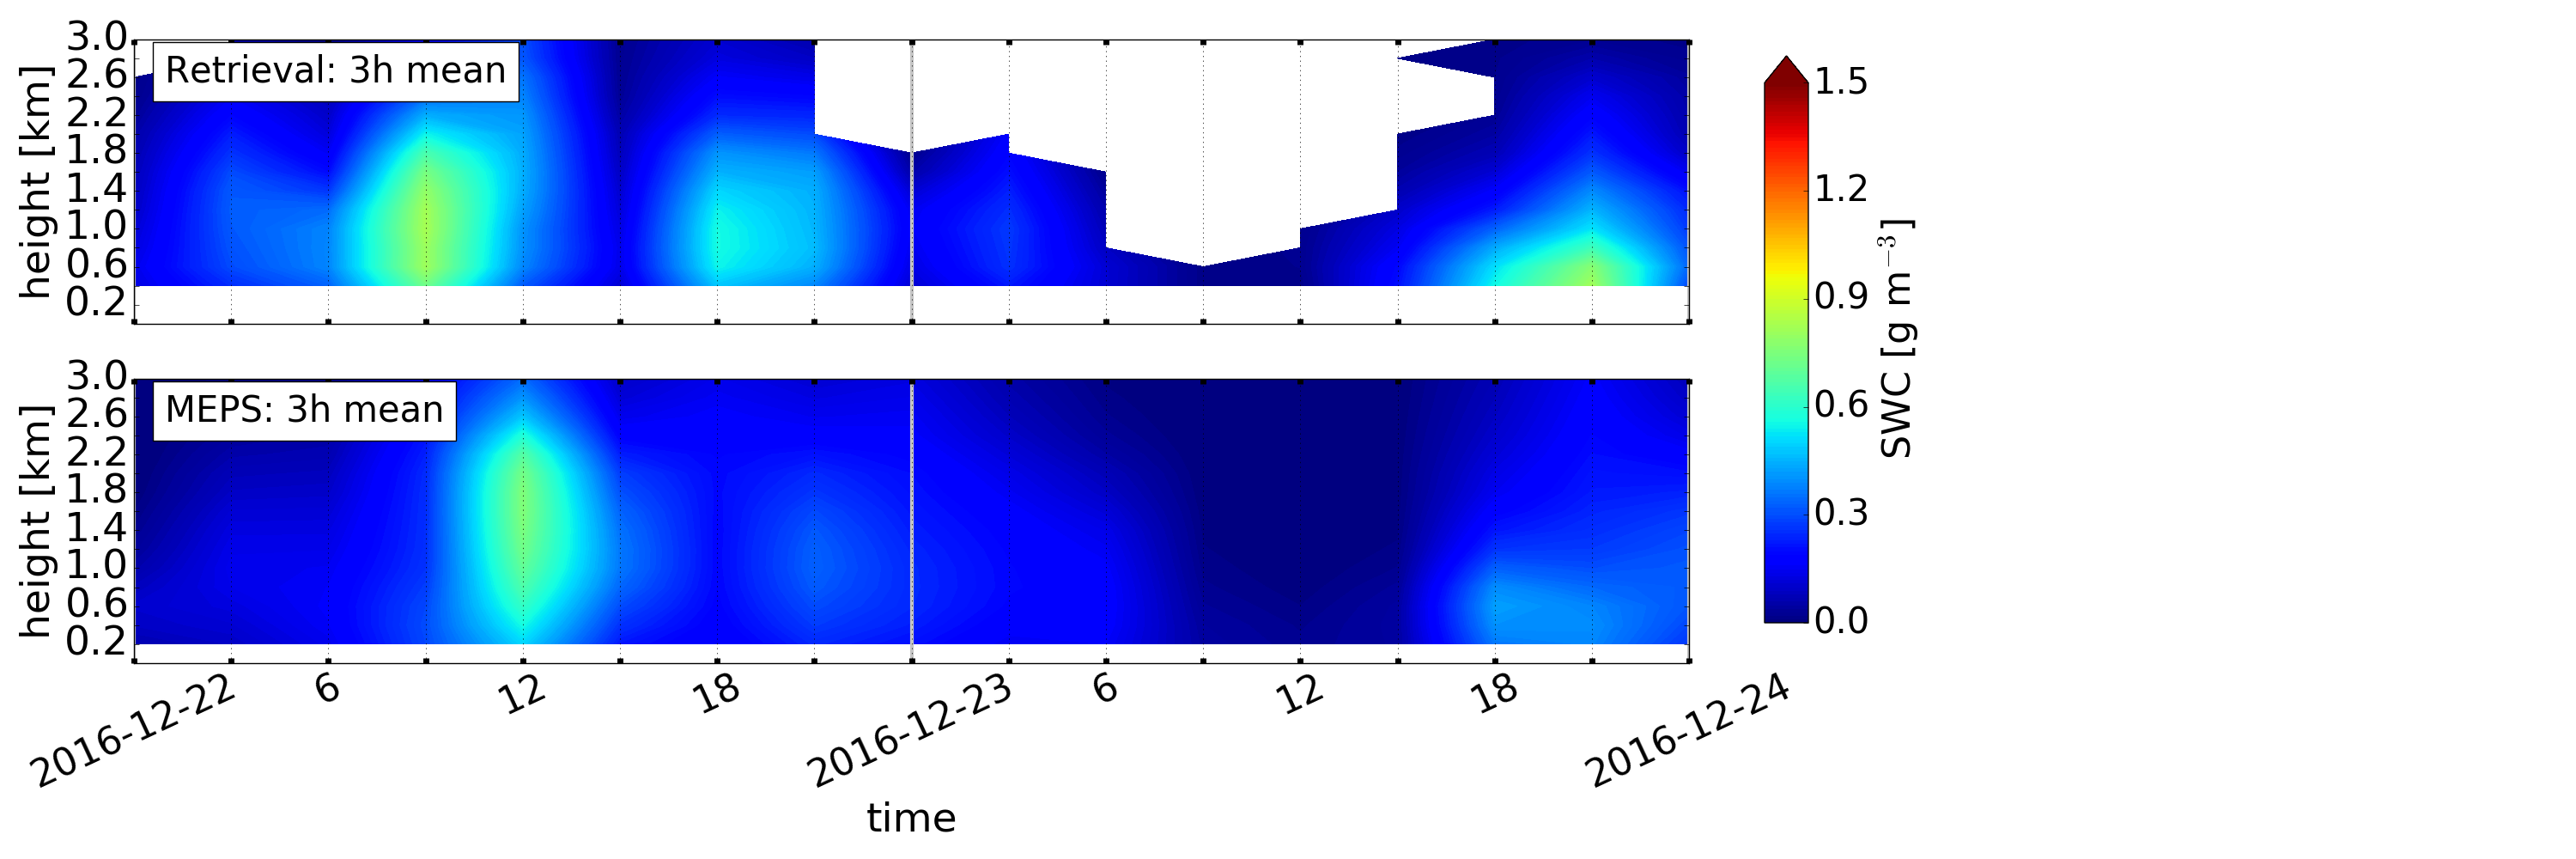
\includegraphics[trim={0.cm 0.8cm 19.cm 0.5cm},clip,width=0.9\textwidth]{./fig_vert_SWC_3h/20161222}
		\caption{}\label{fig:SWC3h:22}
	\end{subfigure}
	\caption{\textit{(As \Cref{fig:SWC21}.)} Initialisation \SI{22}{\dec} at \SI{0}{\UTC}.}\label{fig:SWC22}
\end{figure}
%%%%%%%%%%%%%%%%%%%%%%%%%%%%%%%%%%%%%%%%%%%%%%
%%%%%%%%% image SWC retrieval MEPS 23 %%%%%%%%%%%%%%
\begin{figure}[H]%\ContinuedFloat
	\centering
	% 23/12
	\begin{subfigure}[t]{1.05\textwidth}
		\centering
		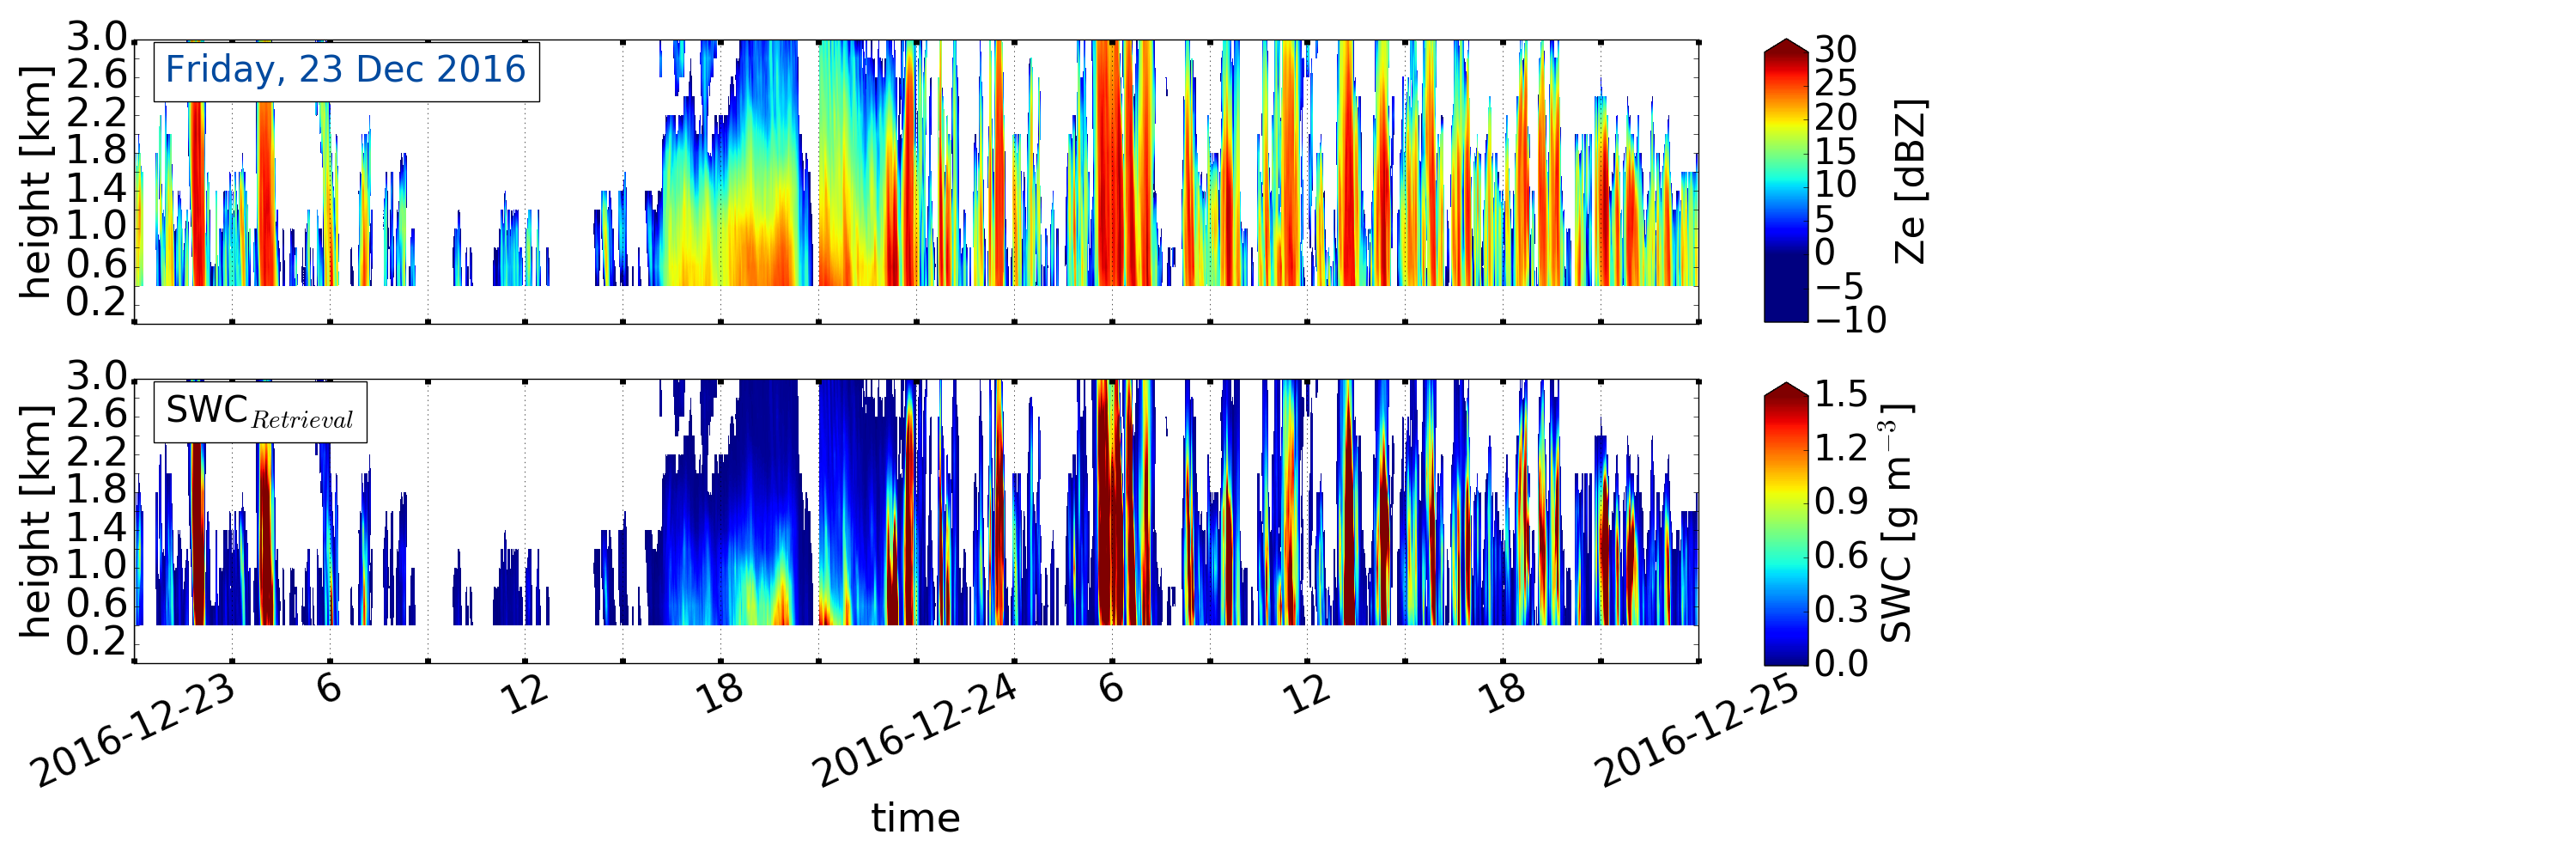
\includegraphics[trim={0.cm 2.2cm 19.cm 0.5cm},clip,width=0.9\textwidth]{./fig_obs_ret/20161223}
		\caption{}\label{fig:SWC:ret_23}
	\end{subfigure}
	% EM
	\begin{subfigure}[t]{1.05\textwidth}
		\centering
		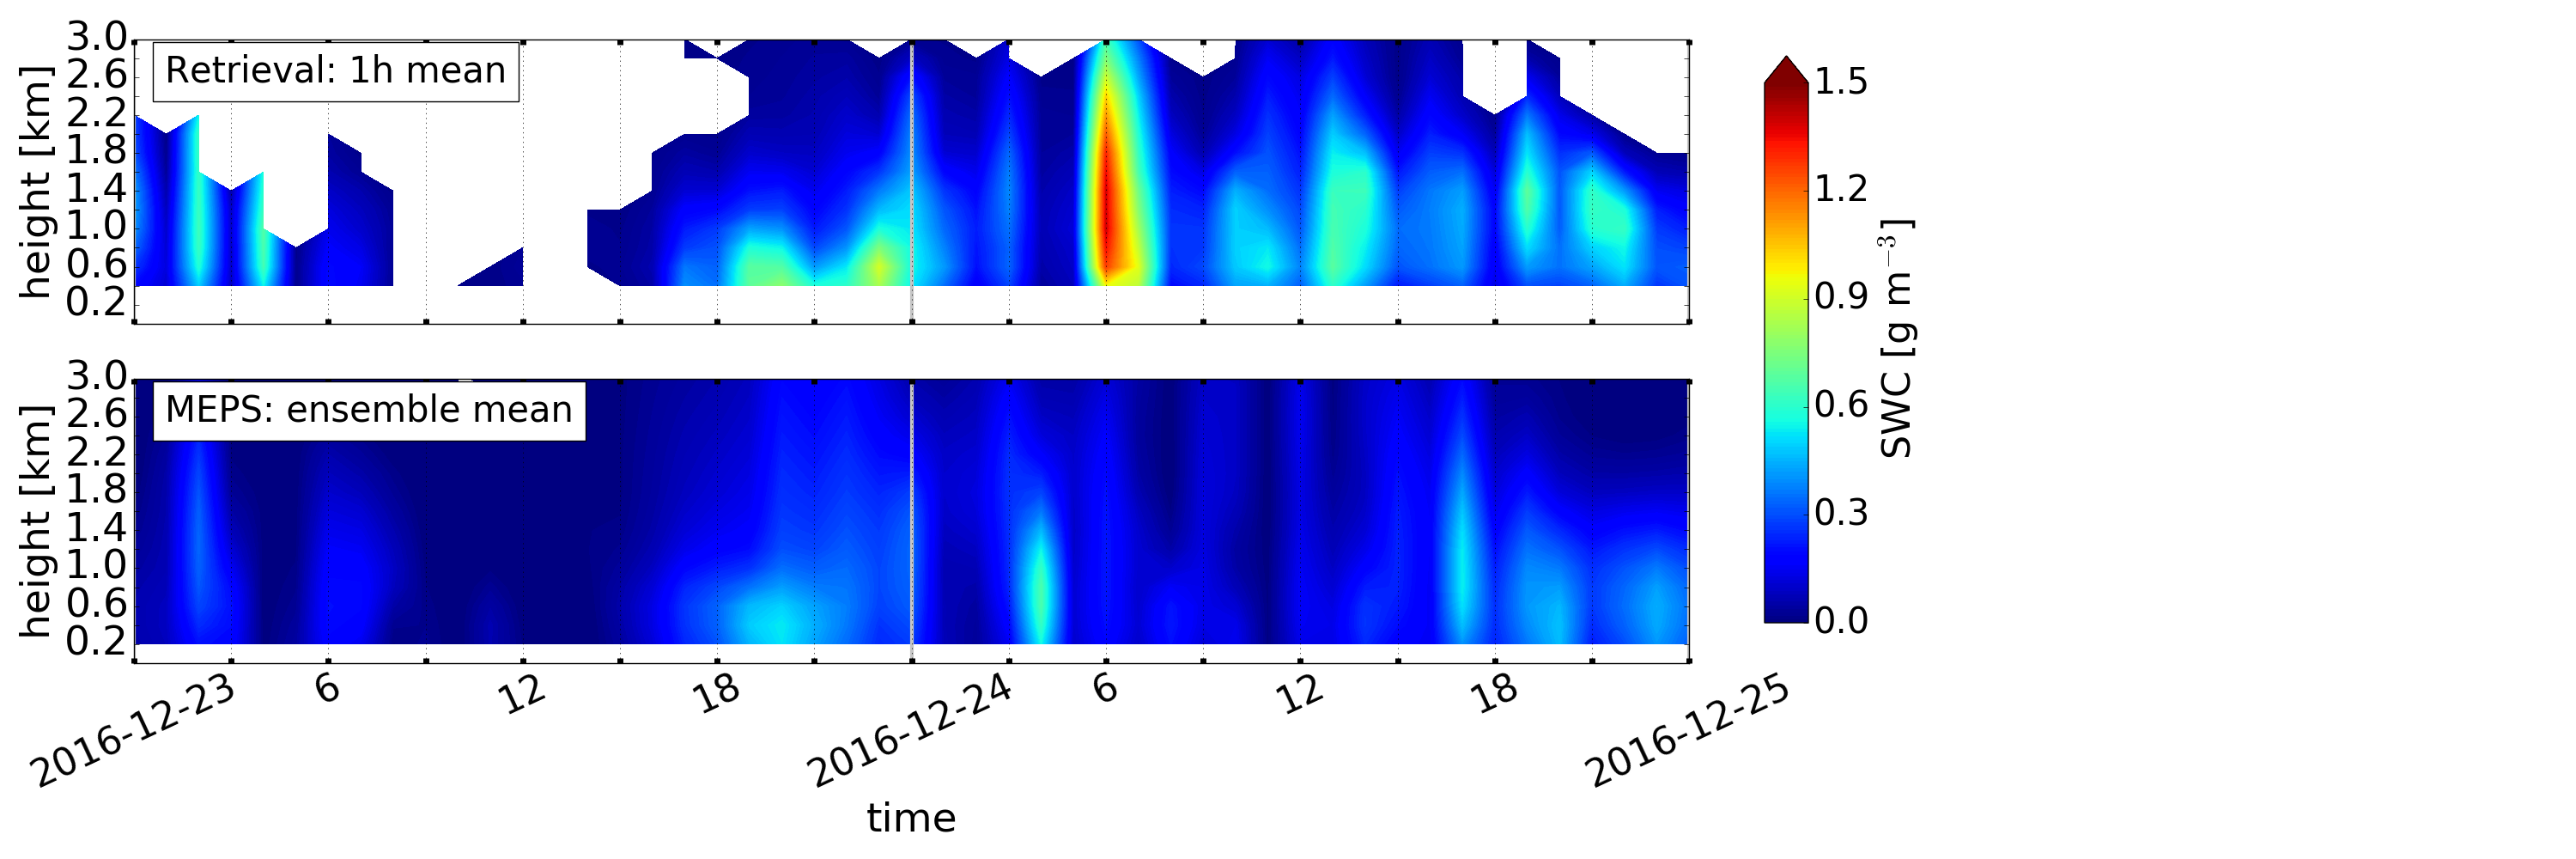
\includegraphics[trim={0.cm 2.2cm 19.cm 0.5cm},clip,width=0.9\textwidth]{./fig_vert_SWC_EM/20161223}
		\caption{}\label{fig:SWC_EM:23}
	\end{subfigure}
	% 3h
	\begin{subfigure}[t]{1.05\textwidth}
		\centering
		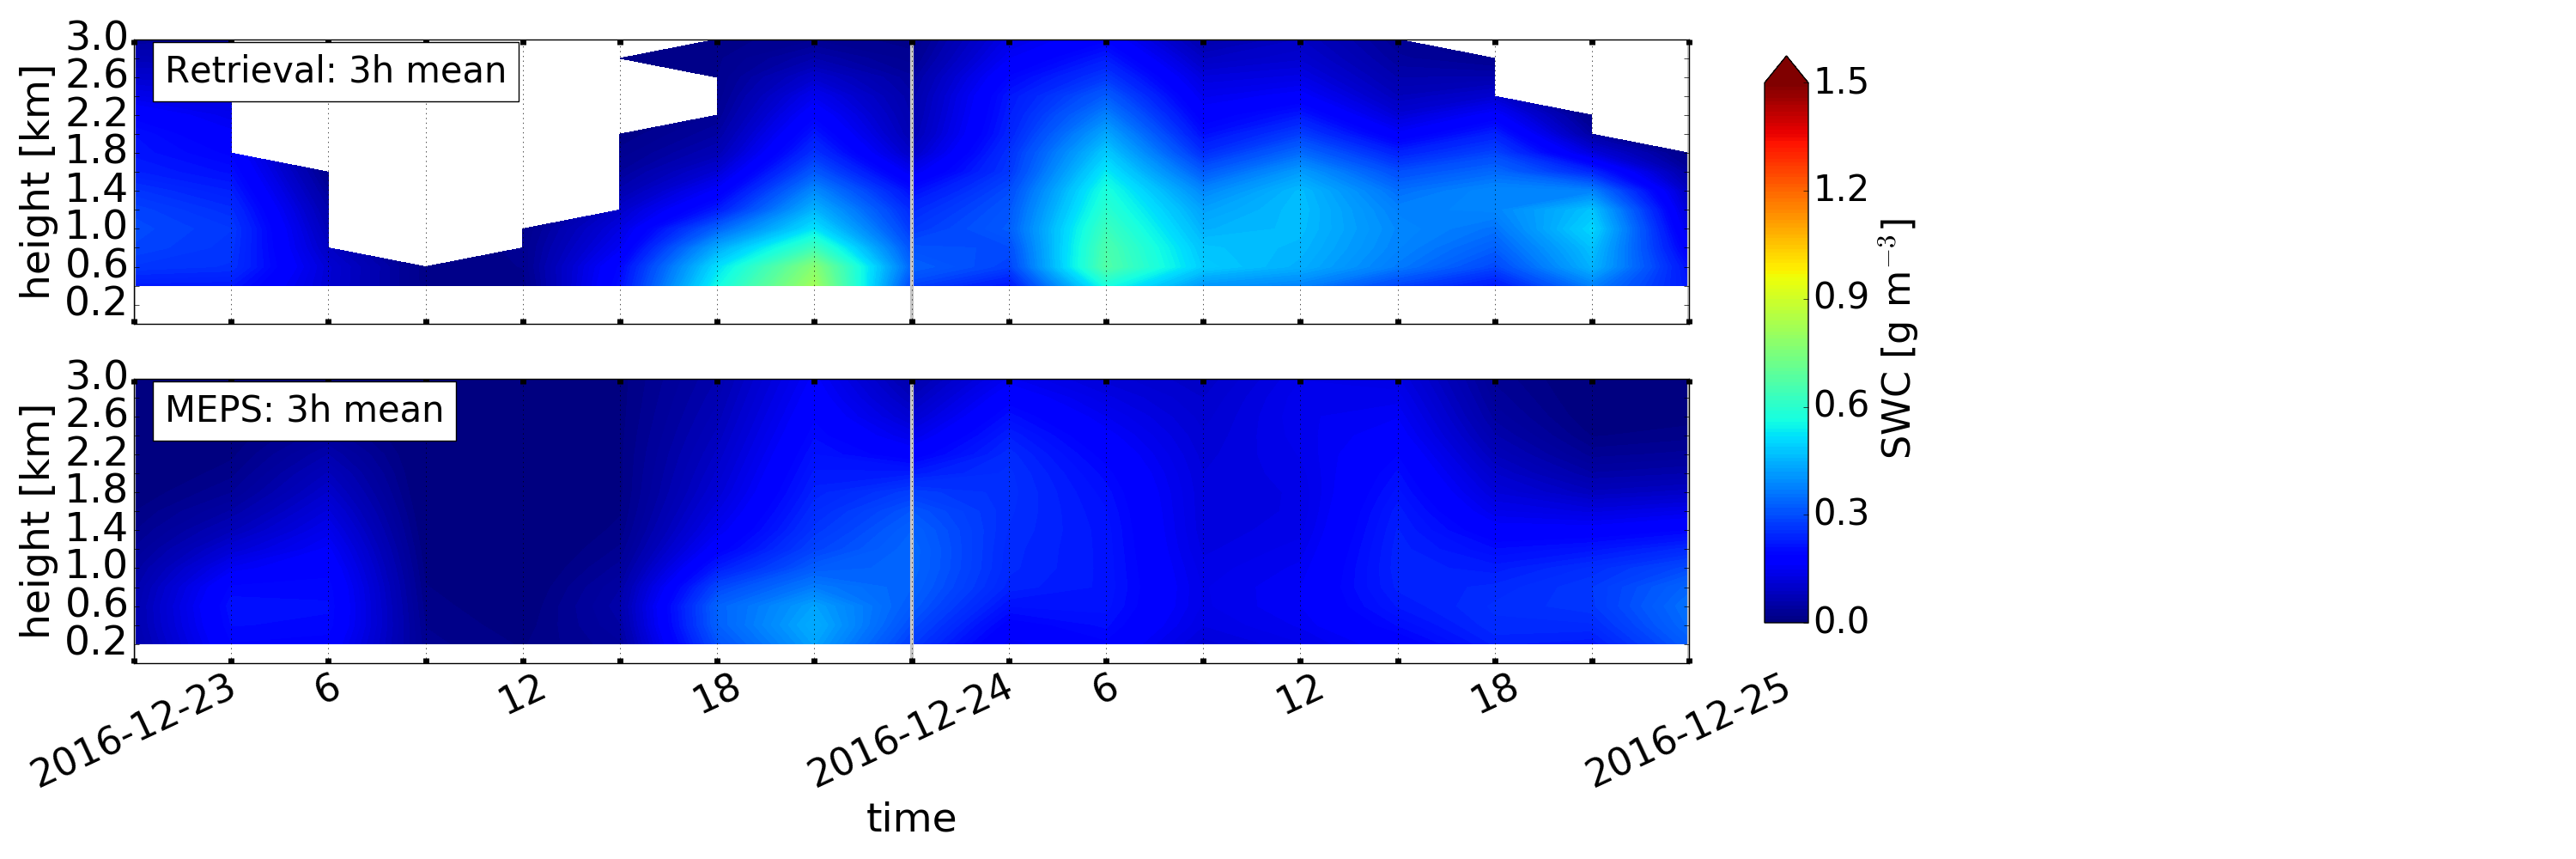
\includegraphics[trim={0.cm 0.8cm 19.cm 0.5cm},clip,width=0.9\textwidth]{./fig_vert_SWC_3h/20161223}
		\caption{}\label{fig:SWC3h:23}
	\end{subfigure}
	\caption{\textit{(As \Cref{fig:SWC21}.)} Initialisation \SI{23}{\dec} at \SI{0}{\UTC}.}\label{fig:SWC23}
\end{figure}
%%%%%%%%%%%%%%%%%%%%%%%%%%%%%%%%%%%%%%%%%%%%%%
%%%%%%%%% image SWC retrieval MEPS 24 %%%%%%%%%%%%%%
\begin{figure}[H]%\ContinuedFloat
	\centering
	% 24/12
	\begin{subfigure}[t]{1.05\textwidth}
		\centering
		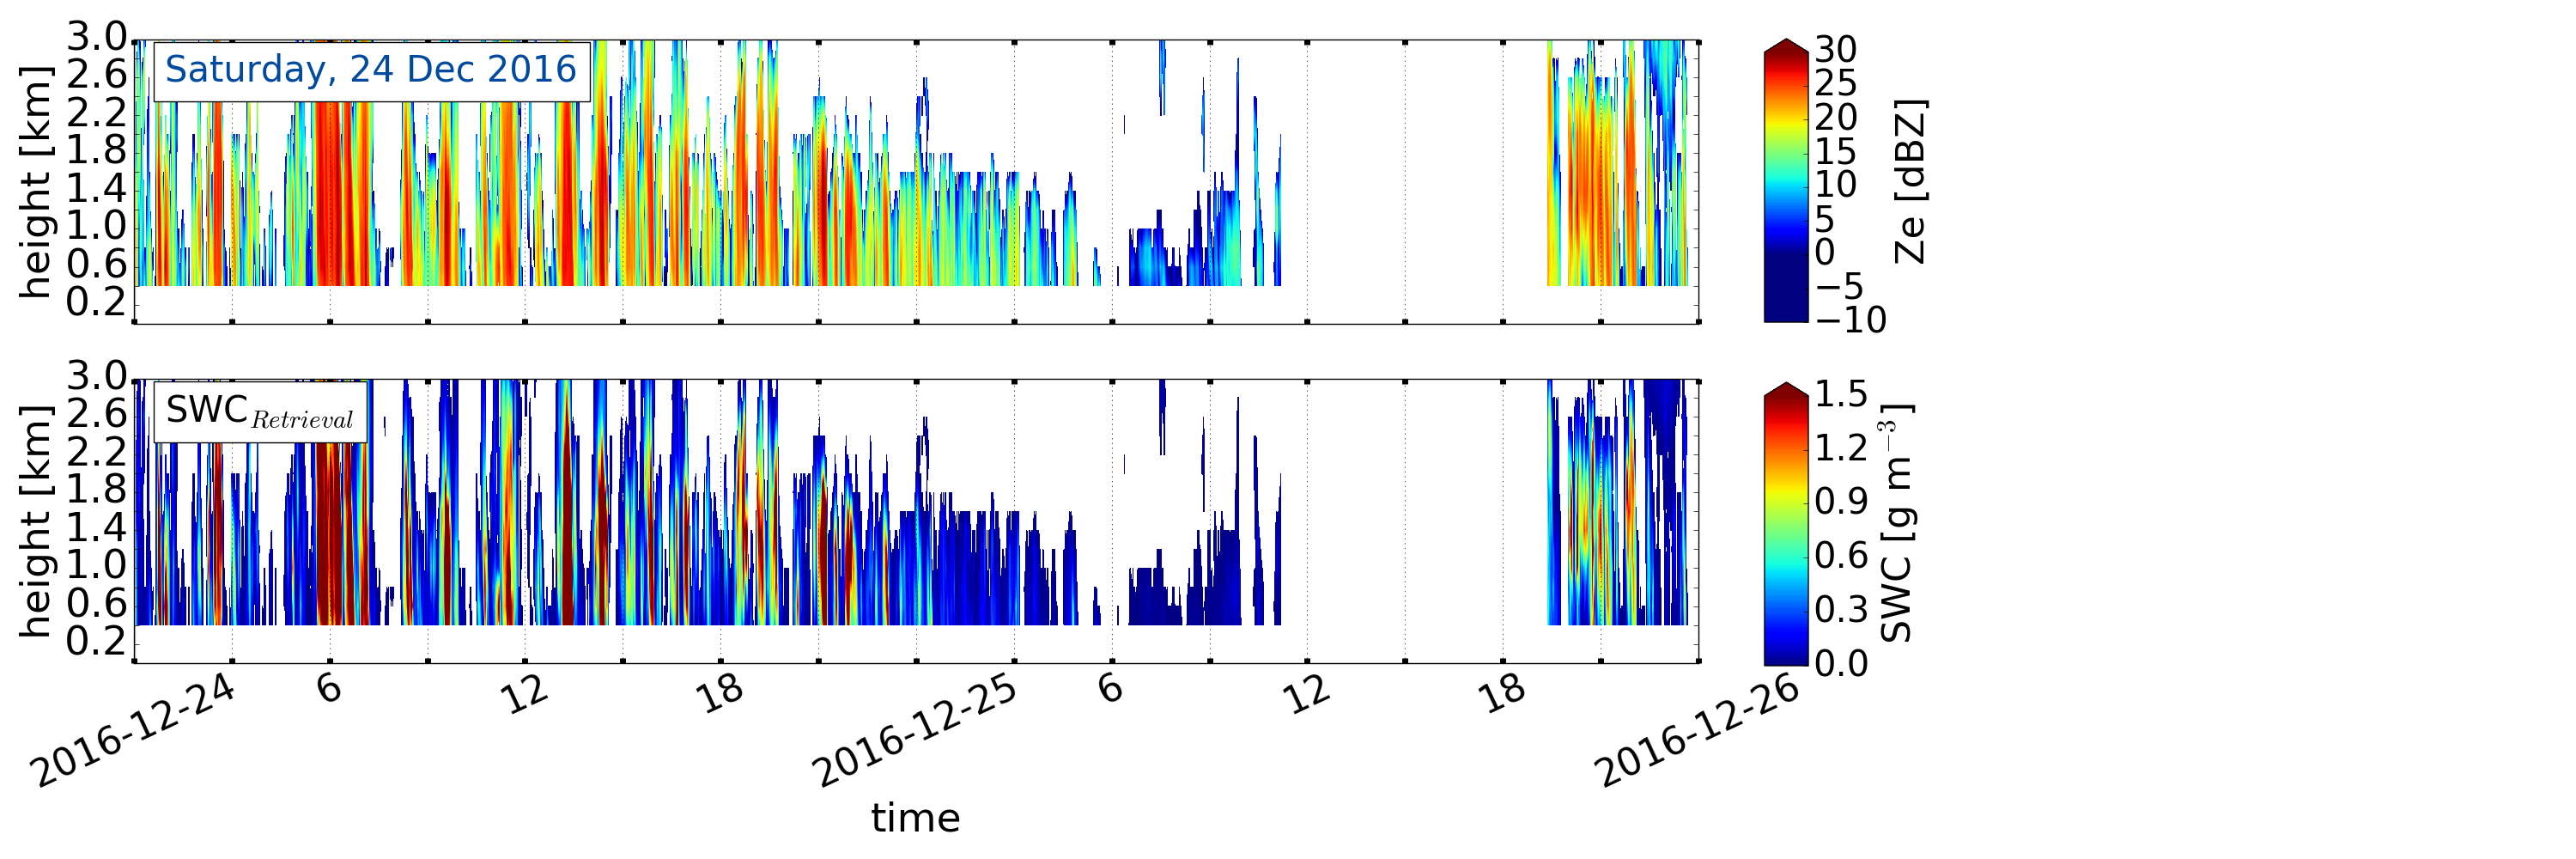
\includegraphics[trim={0.cm 2.2cm 19.cm 0.5cm},clip,width=0.9\textwidth]{./fig_obs_ret/20161224}
		\caption{}\label{fig:SWC:ret_24}
	\end{subfigure}
	% EM
	\begin{subfigure}[t]{1.05\textwidth}
		\centering
		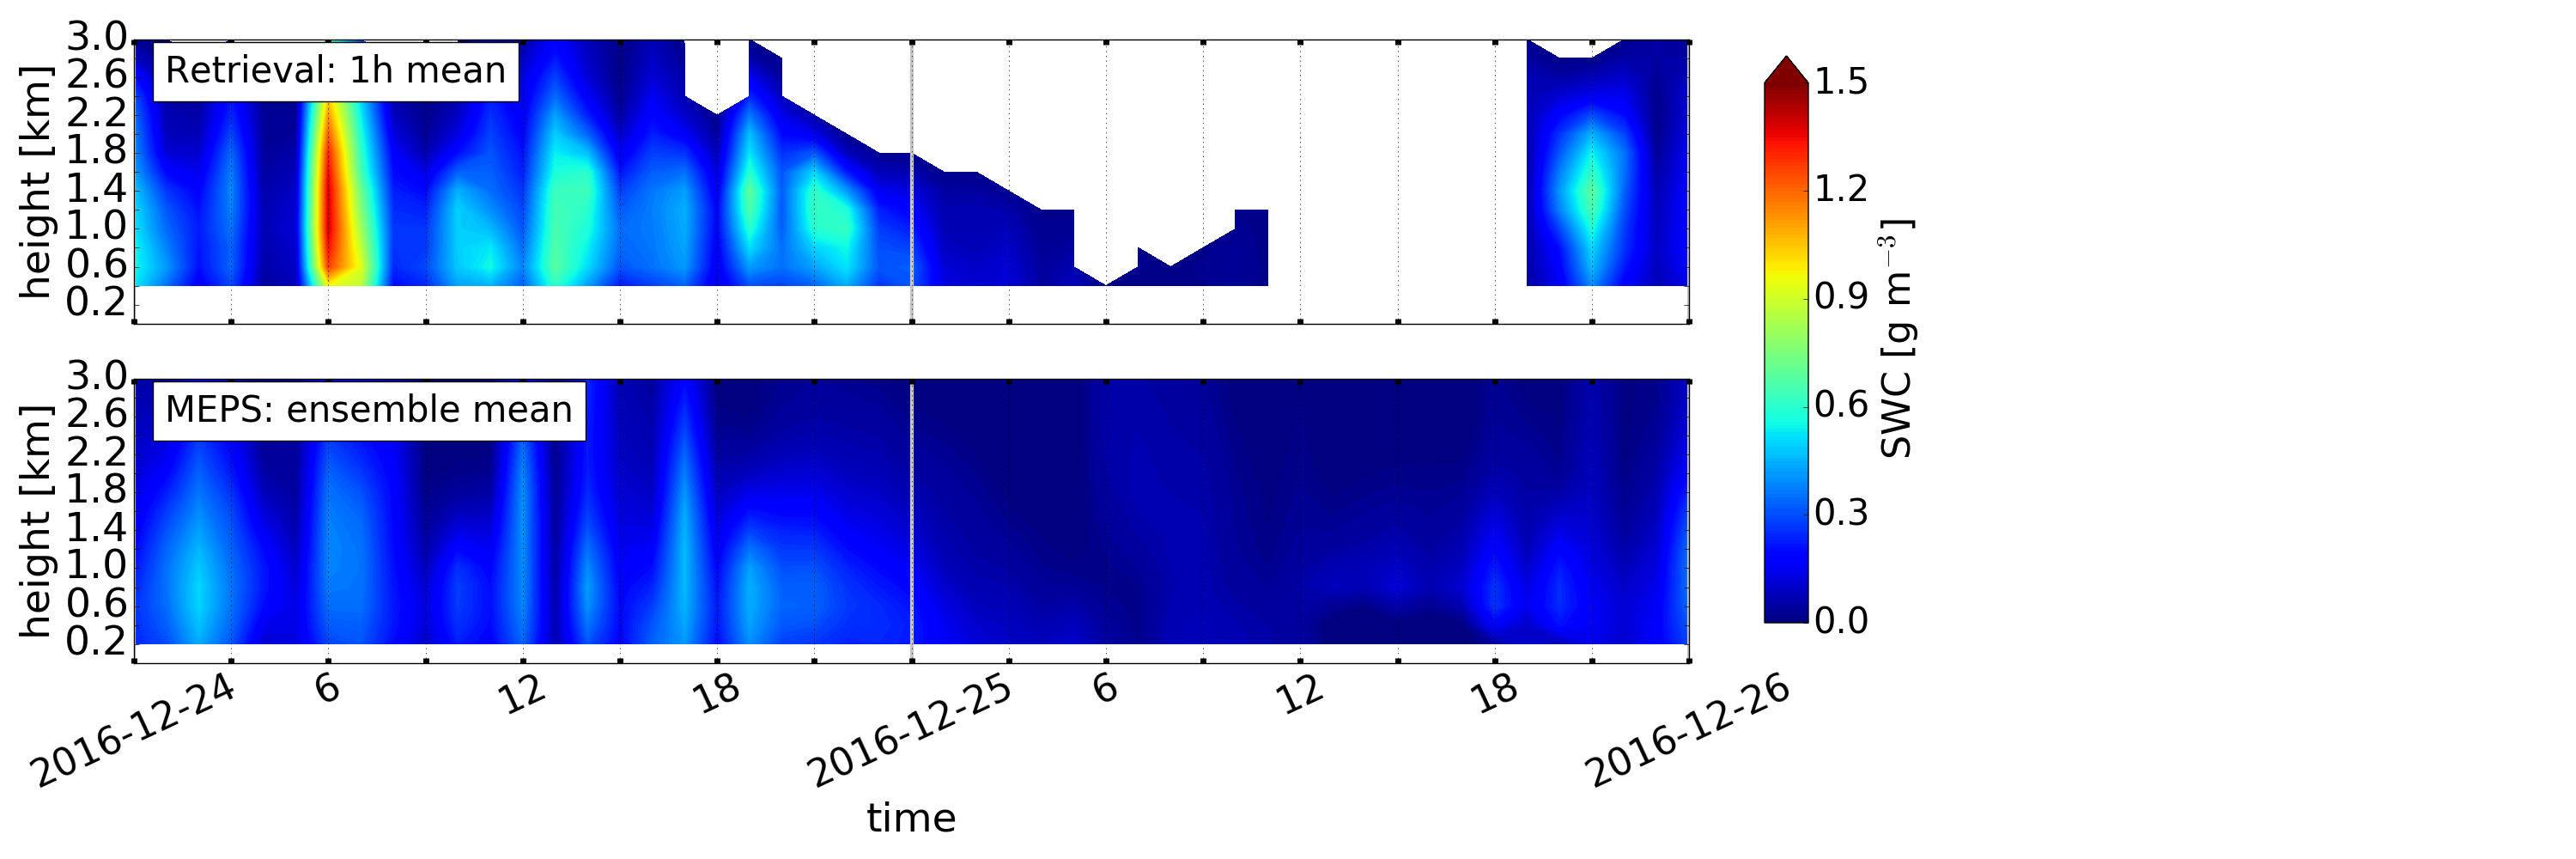
\includegraphics[trim={0.cm 2.2cm 19.cm 0.5cm},clip,width=0.9\textwidth]{./fig_vert_SWC_EM/20161224}
		\caption{}\label{fig:SWC_EM:24}
	\end{subfigure}
	% 3h
	\begin{subfigure}[t]{1.05\textwidth}
		\centering
		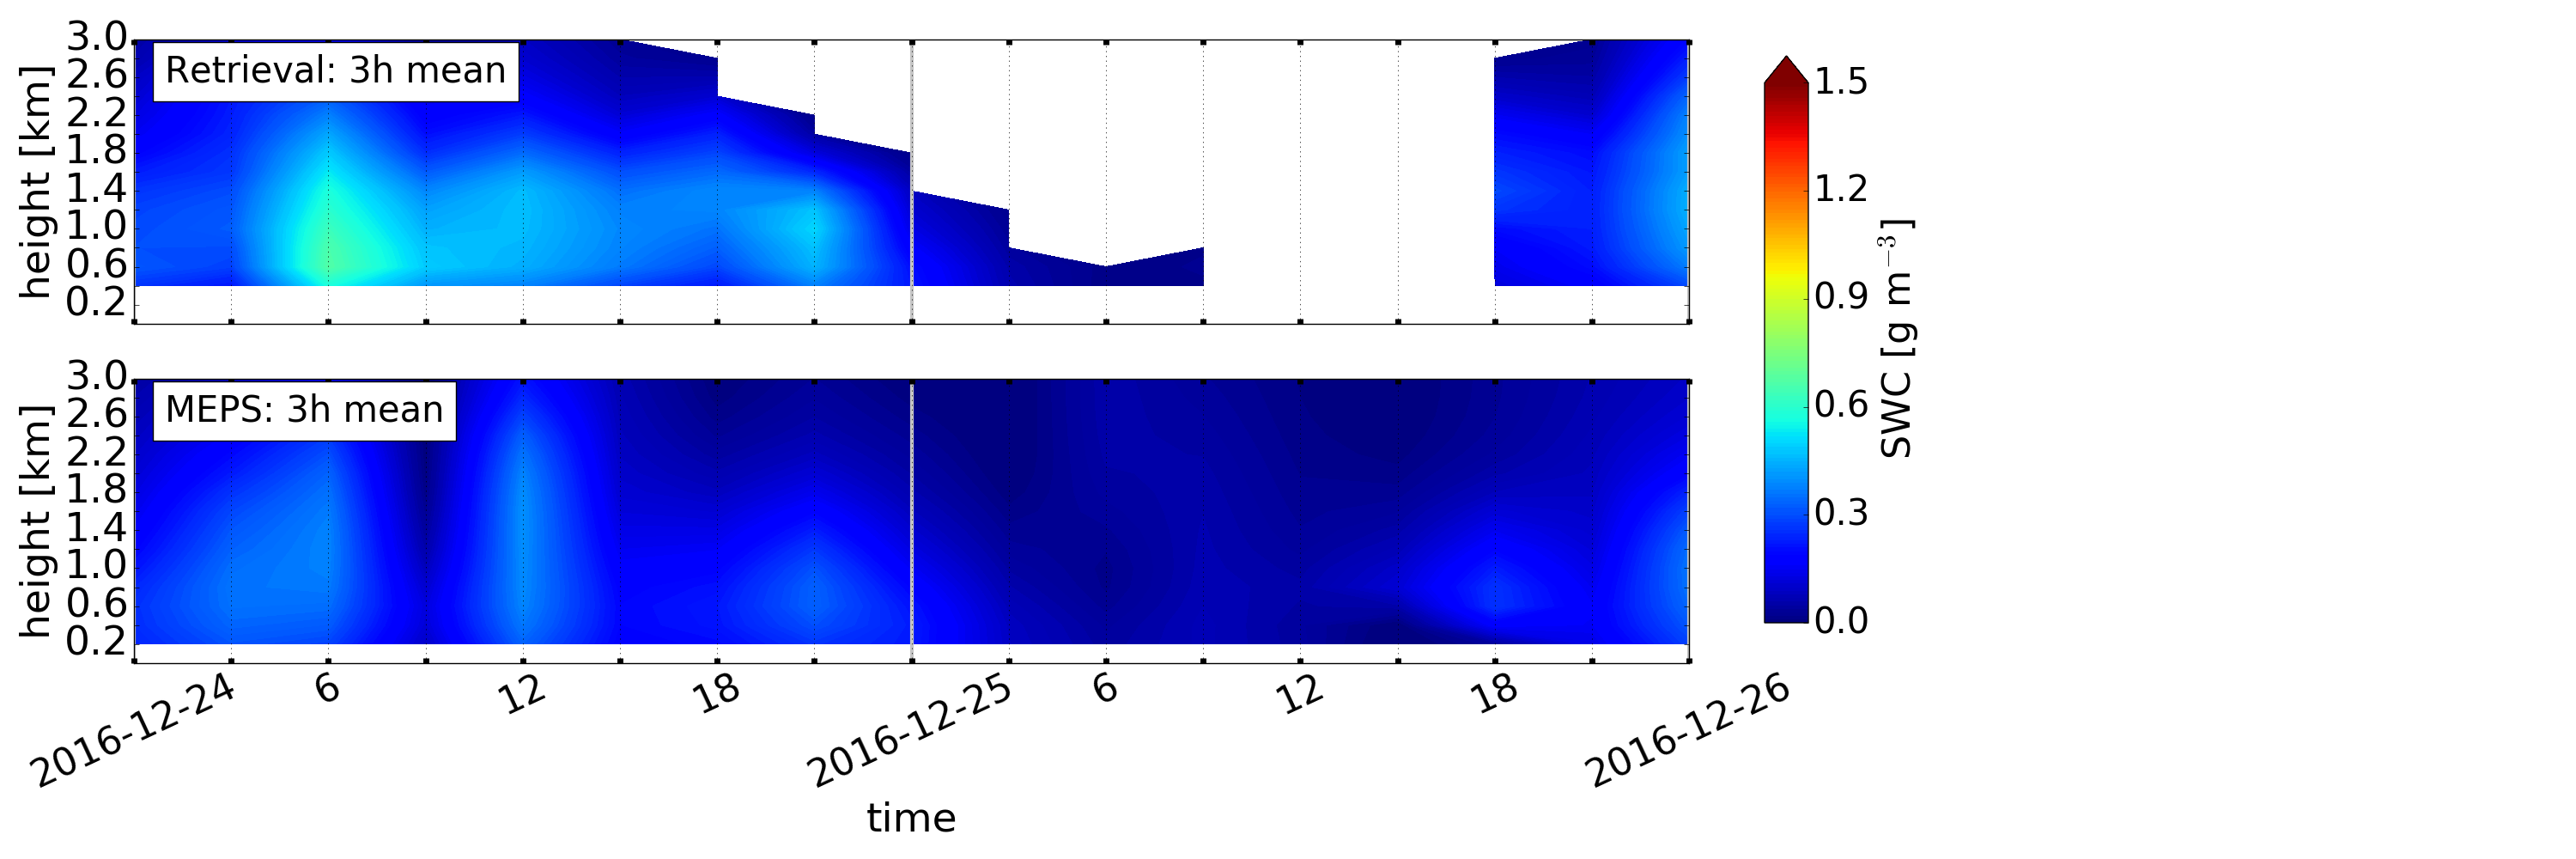
\includegraphics[trim={0.cm 0.8cm 19.cm 0.5cm},clip,width=0.9\textwidth]{./fig_vert_SWC_3h/20161224}
		\caption{}\label{fig:SWC3h:24}
	\end{subfigure}
	\caption{\textit{(As \Cref{fig:SWC21}.)} Initialisation \SI{24}{\dec} at \SI{0}{\UTC}.}\label{fig:SWC24}
\end{figure}
%%%%%%%%%%%%%%%%%%%%%%%%%%%%%%%%%%%%%%%%%%%%%%
%%%%%%%%% image SWC retrieval MEPS 25 %%%%%%%%%%%%%%
\begin{figure}[H]%\ContinuedFloat
	\centering
	% 25/12
	\begin{subfigure}[t]{1.05\textwidth}
		\centering
		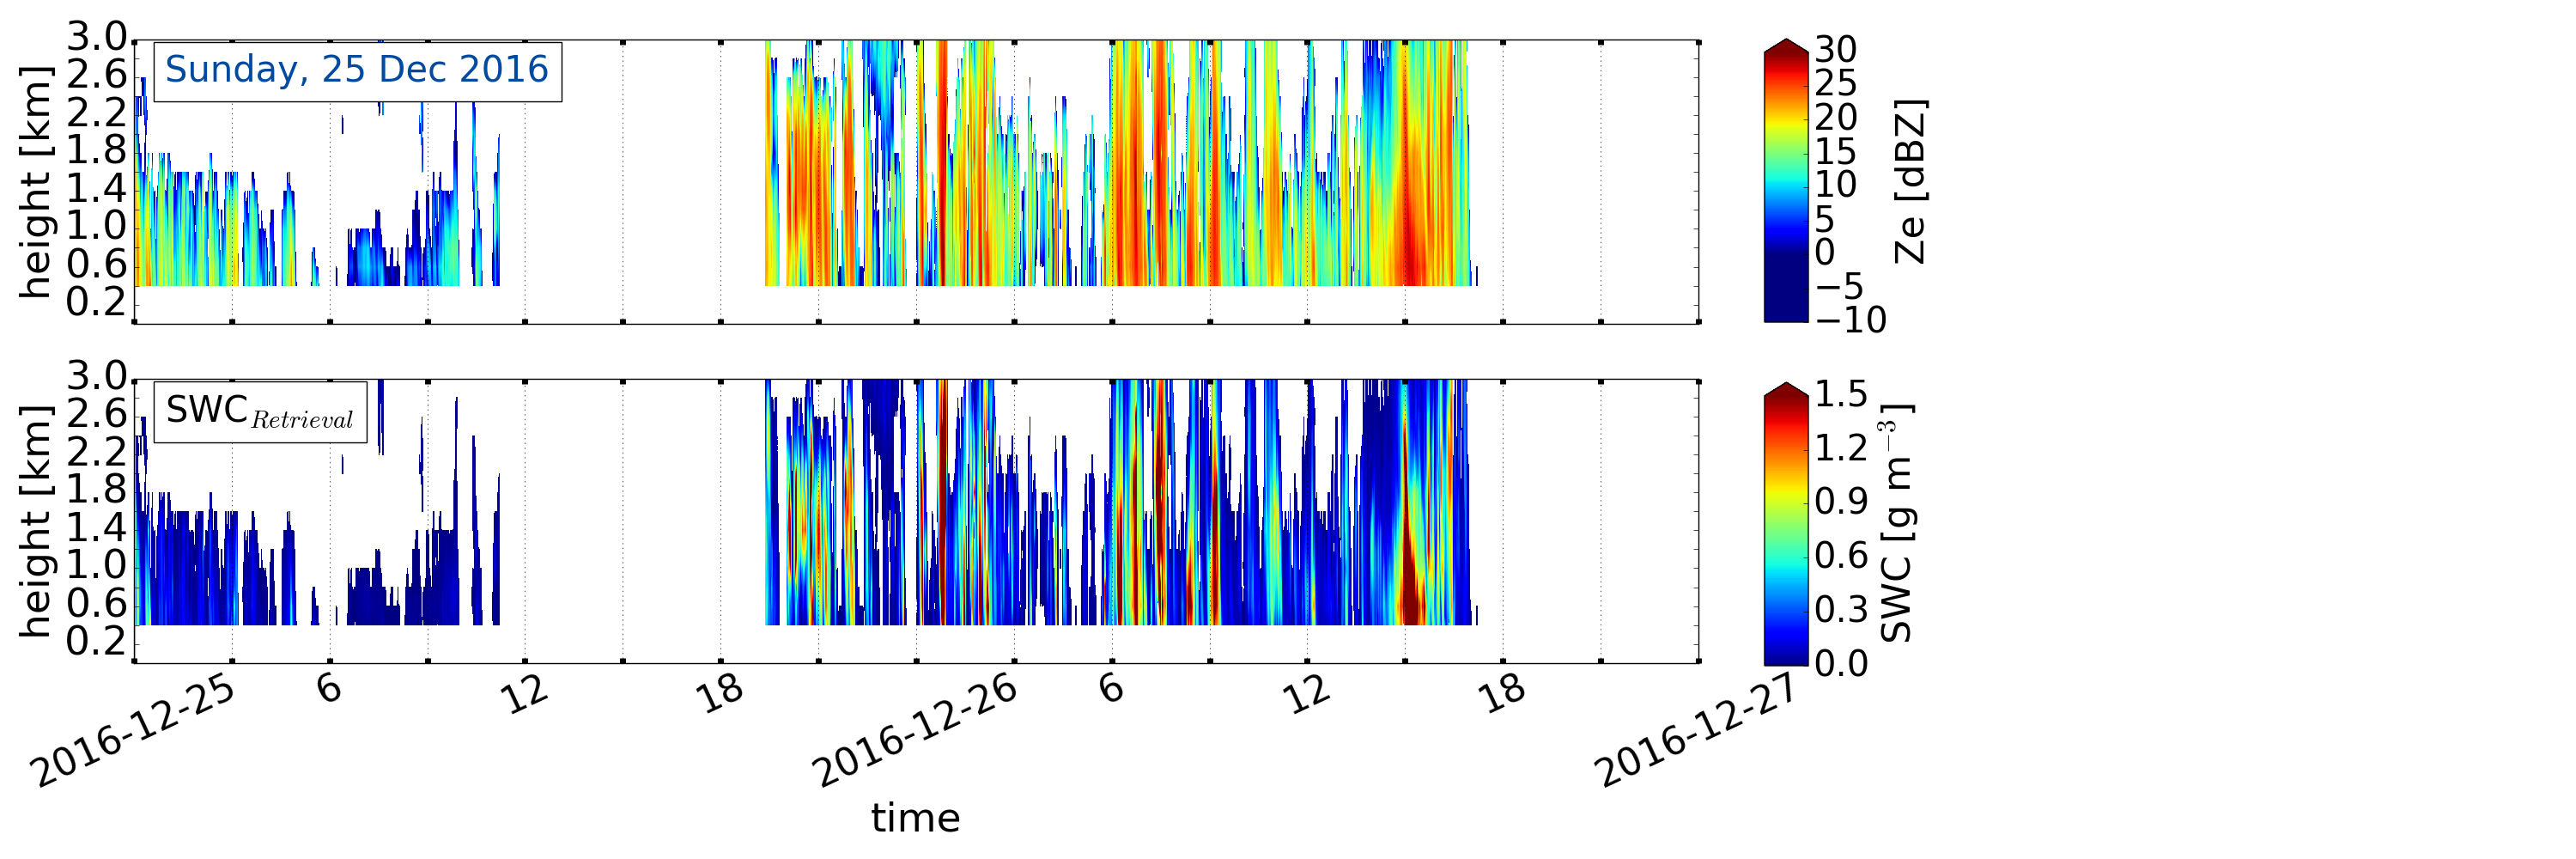
\includegraphics[trim={0.cm 2.2cm 19.cm 0.5cm},clip,width=0.9\textwidth]{./fig_obs_ret/20161225}
		\caption{}\label{fig:SWC:ret_25}
	\end{subfigure}
	% EM
	\begin{subfigure}[t]{1.05\textwidth}
		\centering
		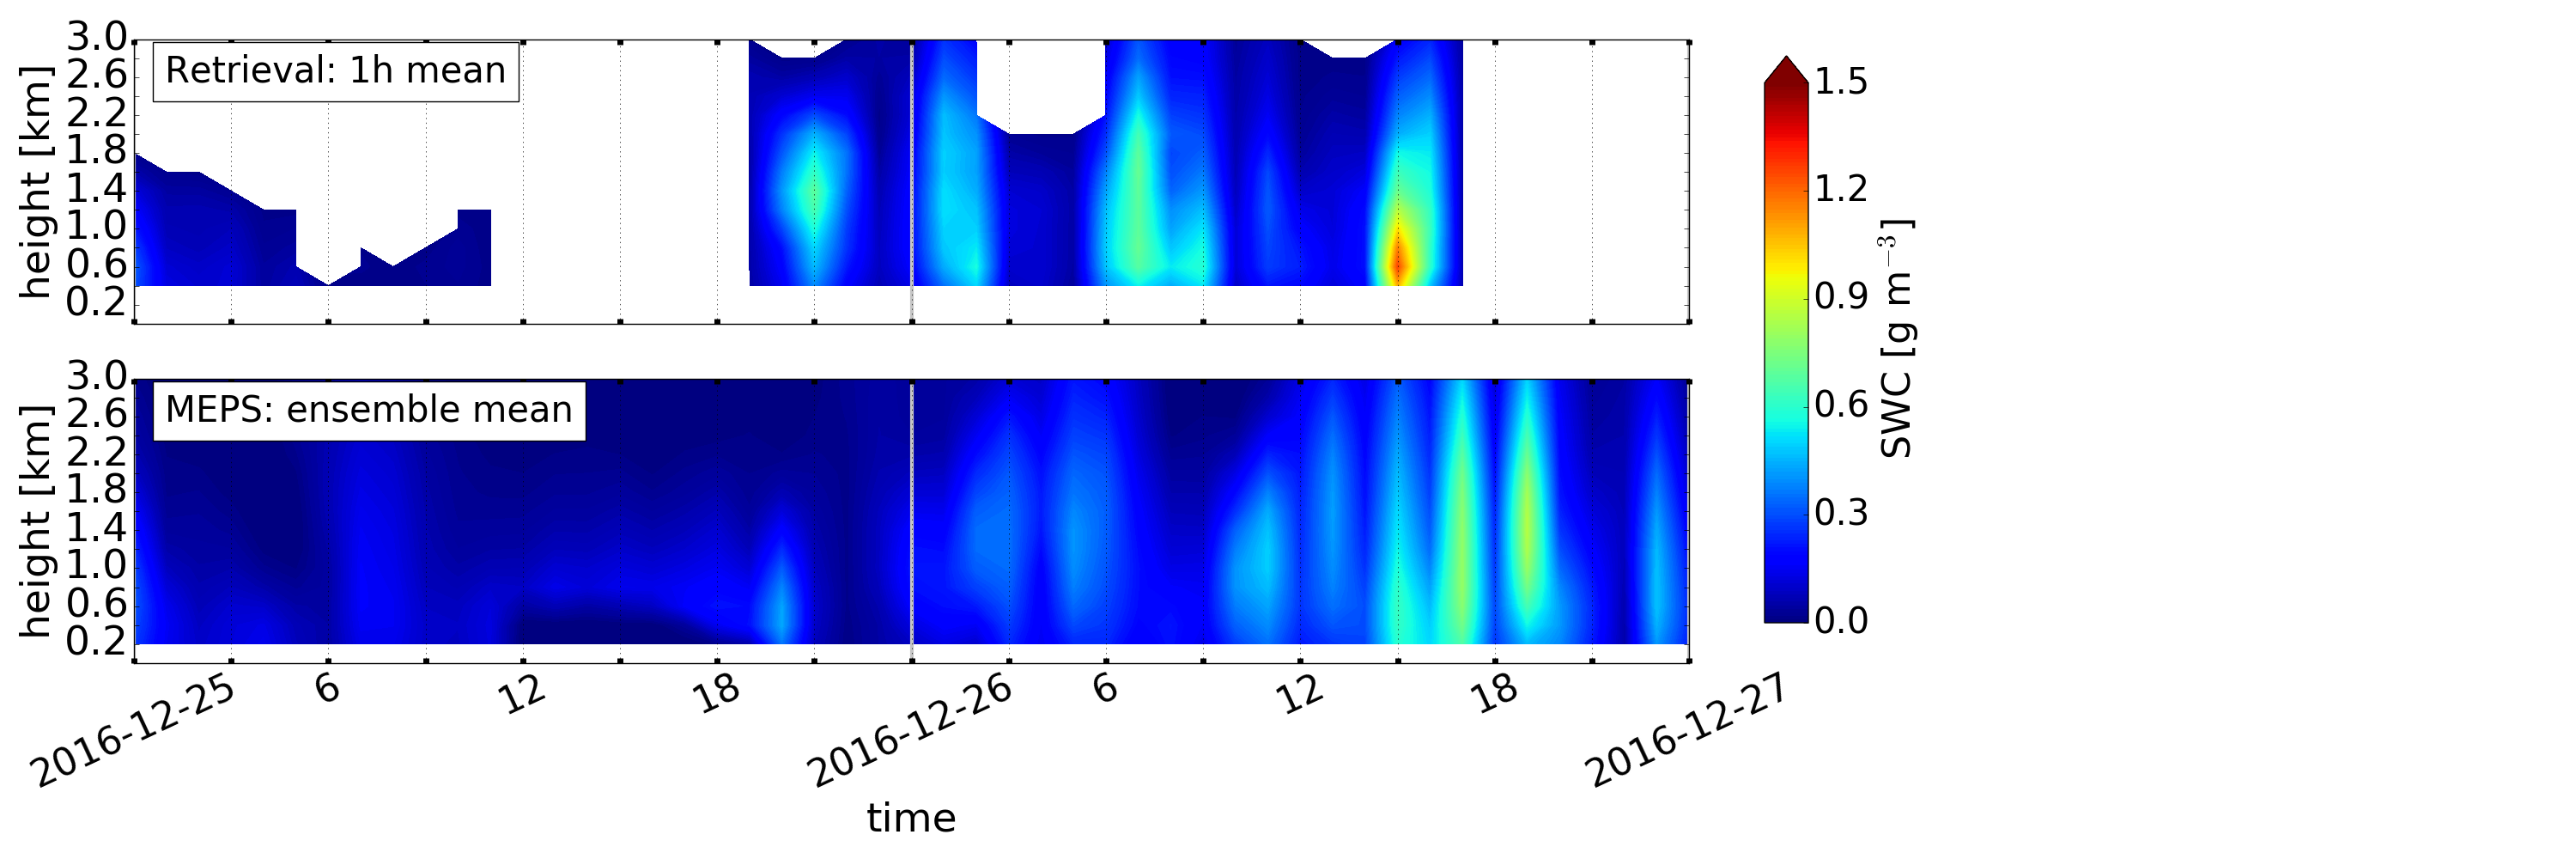
\includegraphics[trim={0.cm 2.2cm 19.cm 0.5cm},clip,width=0.9\textwidth]{./fig_vert_SWC_EM/20161225}
		\caption{}\label{fig:SWC_EM:25}
	\end{subfigure}
	% 3h
	\begin{subfigure}[t]{1.05\textwidth}
		\centering
		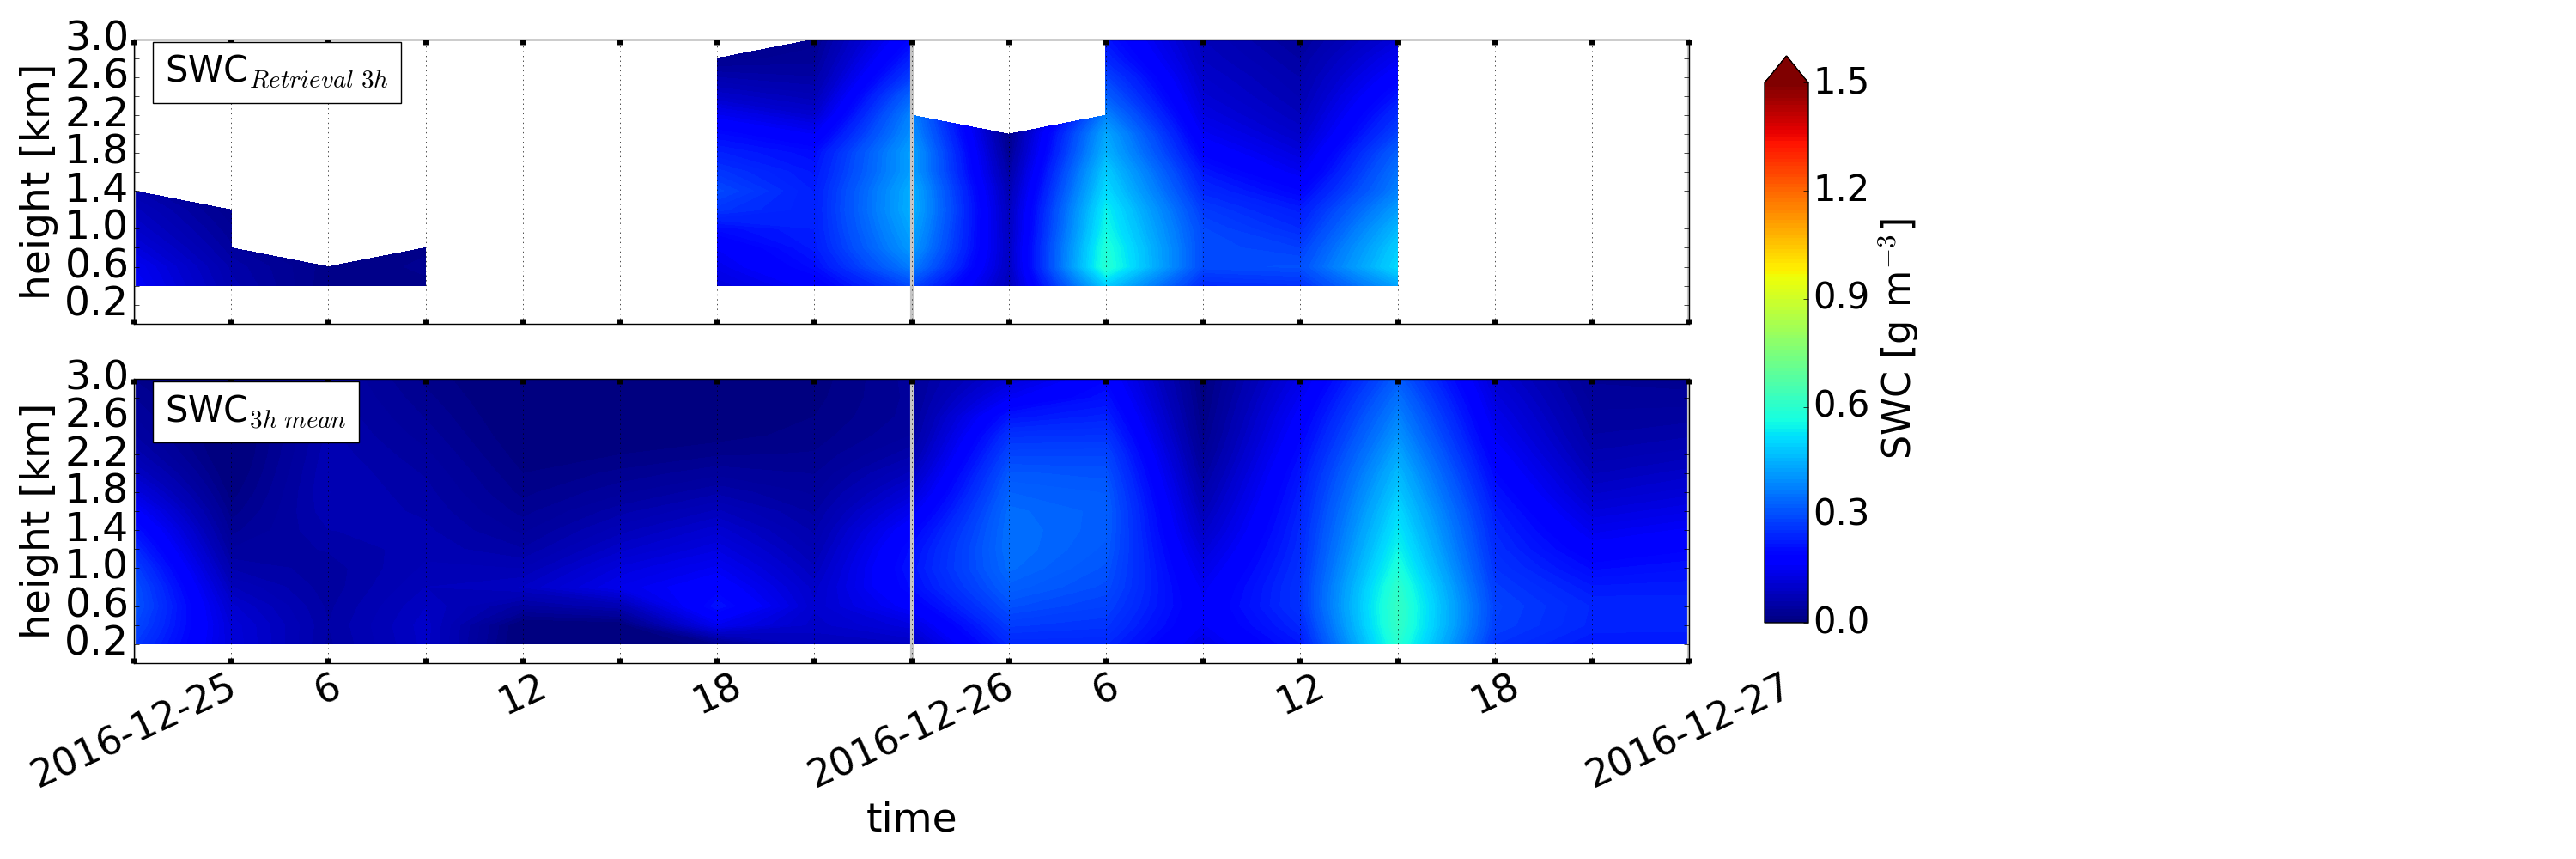
\includegraphics[trim={0.cm 0.8cm 19.cm 0.5cm},clip,width=0.9\textwidth]{./fig_vert_SWC_3h/20161225}
		\caption{}\label{fig:SWC3h:25}
	\end{subfigure}
	\caption{\textit{(As \Cref{fig:SWC21}.)} Initialisation \SI{25}{\dec} at \SI{0}{\UTC}.}\label{fig:SWC25}
\end{figure}
%%%%%%%%% image SWC retrieval MEPS 26 %%%%%%%%%%%%%%
\begin{figure}[H]%\ContinuedFloat
	\centering
	% 25/12
	\begin{subfigure}[t]{1.05\textwidth}
		\centering
		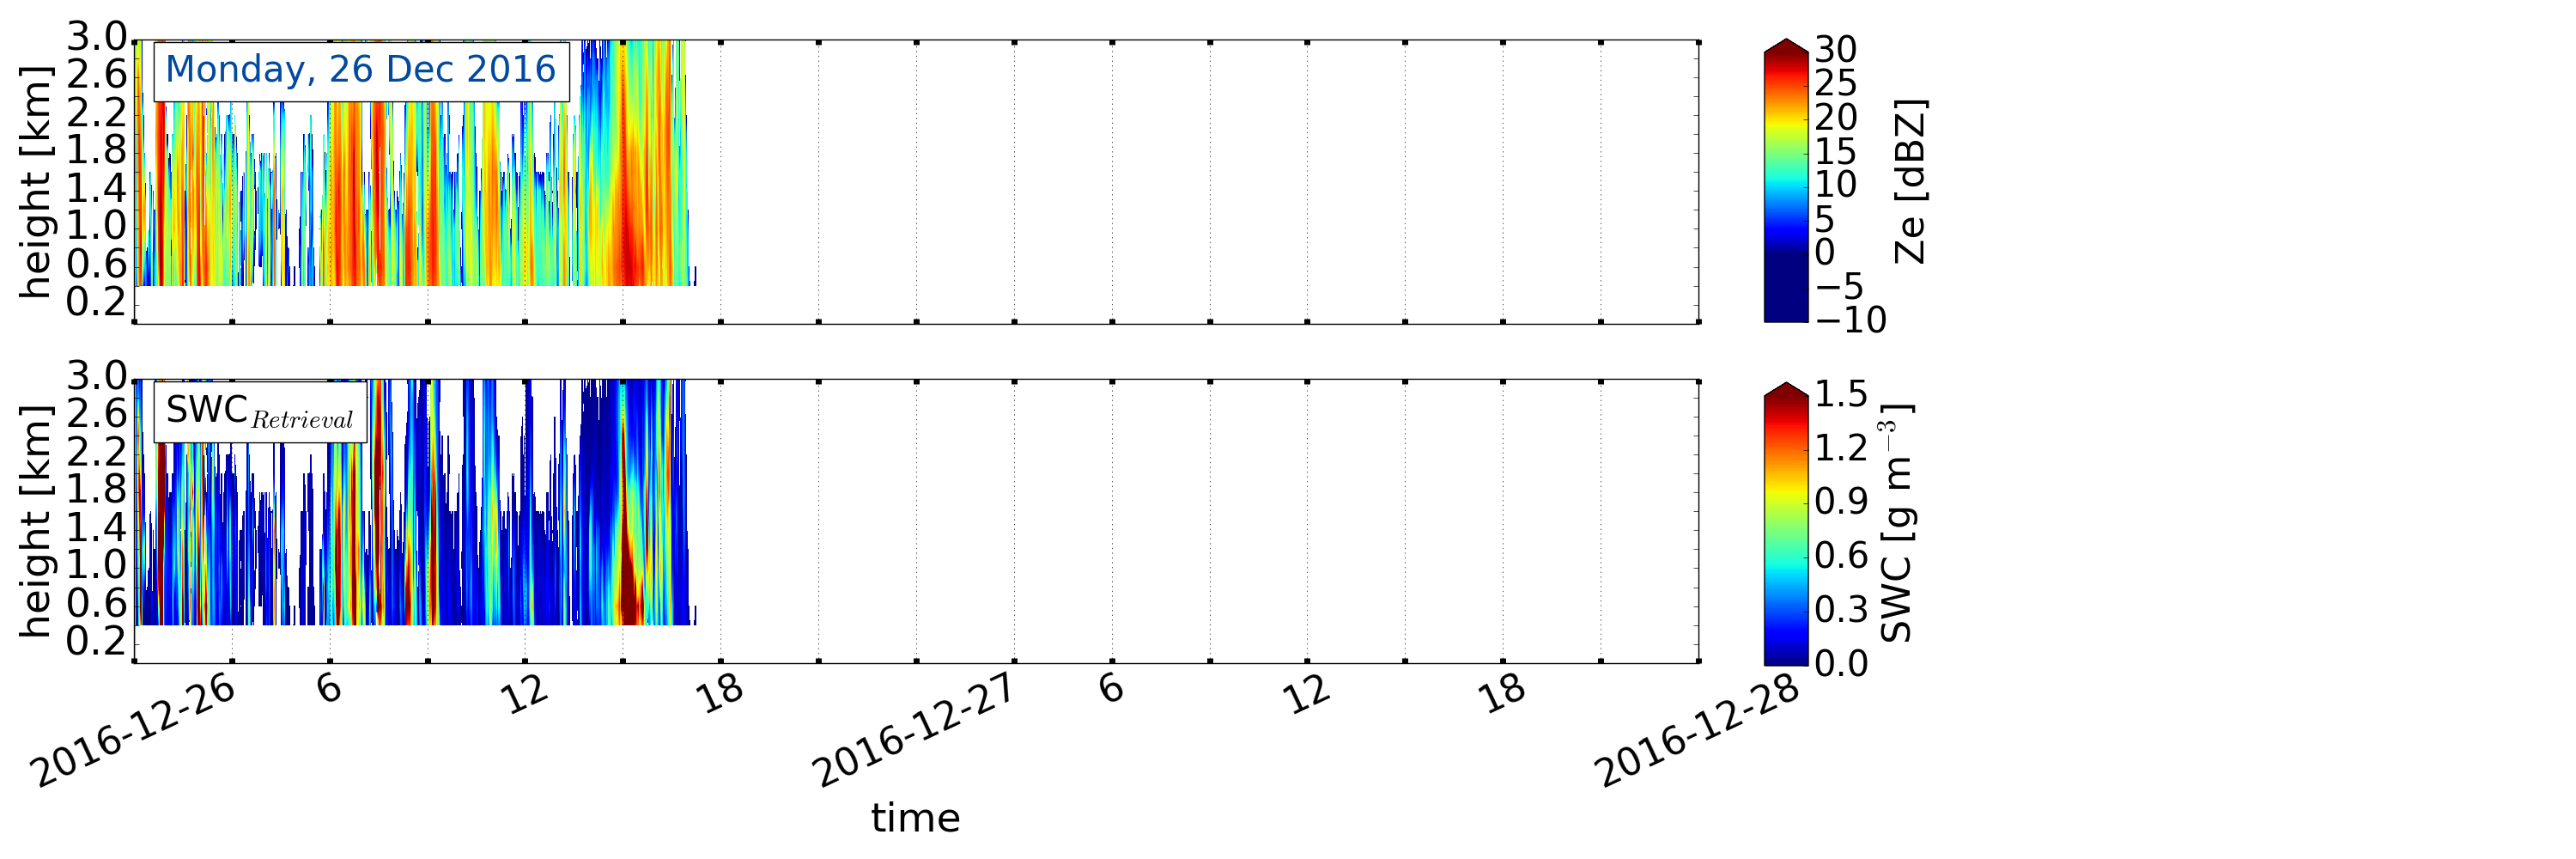
\includegraphics[trim={0.cm 2.2cm 19.cm 0.5cm},clip,width=0.9\textwidth]{./fig_obs_ret/20161226}
		\caption{}\label{fig:SWC:ret_26}
	\end{subfigure}
	% EM
	\begin{subfigure}[t]{1.05\textwidth}
		\centering
		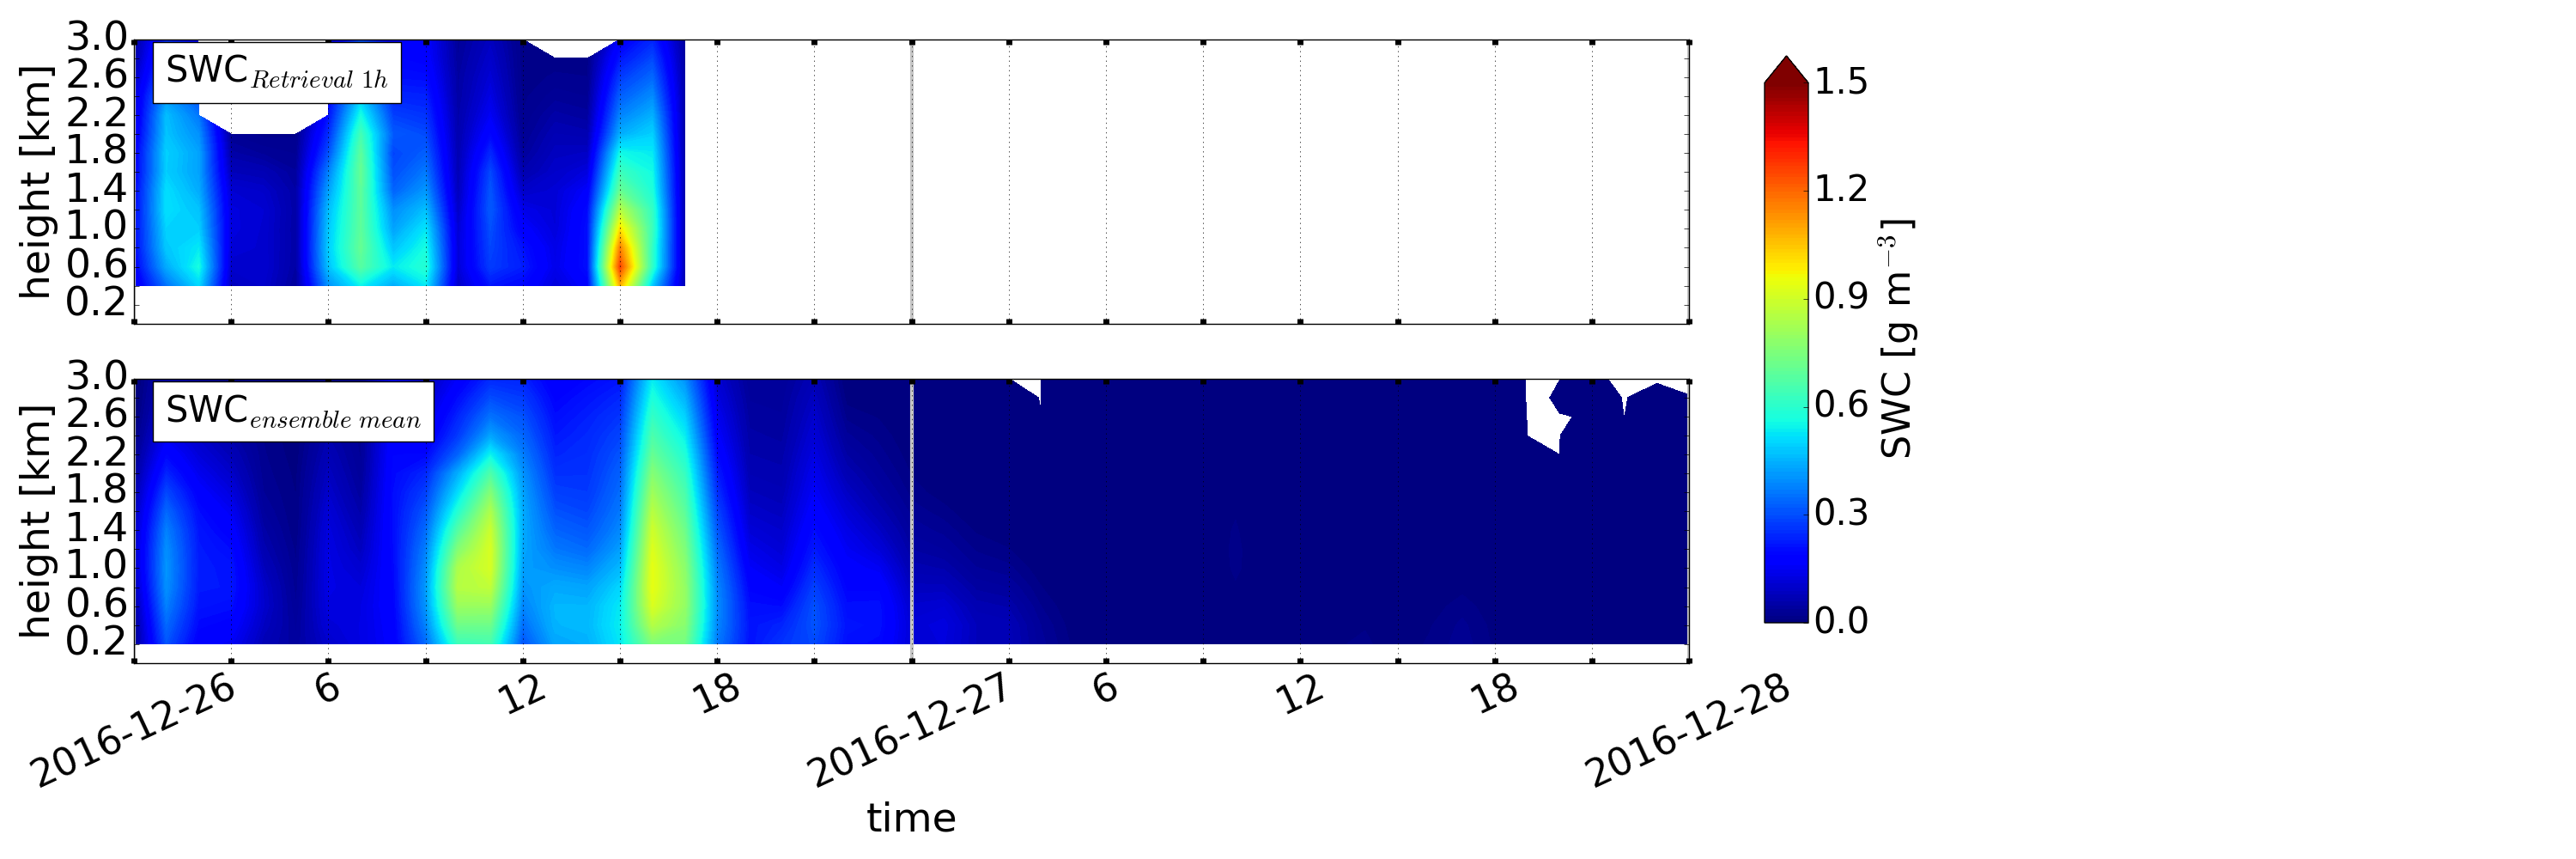
\includegraphics[trim={0.cm 2.2cm 19.cm 0.5cm},clip,width=0.9\textwidth]{./fig_vert_SWC_EM/20161226}
		\caption{}\label{fig:SWC_EM:26}
	\end{subfigure}
	% 3h
	\begin{subfigure}[t]{1.05\textwidth}
		\centering
		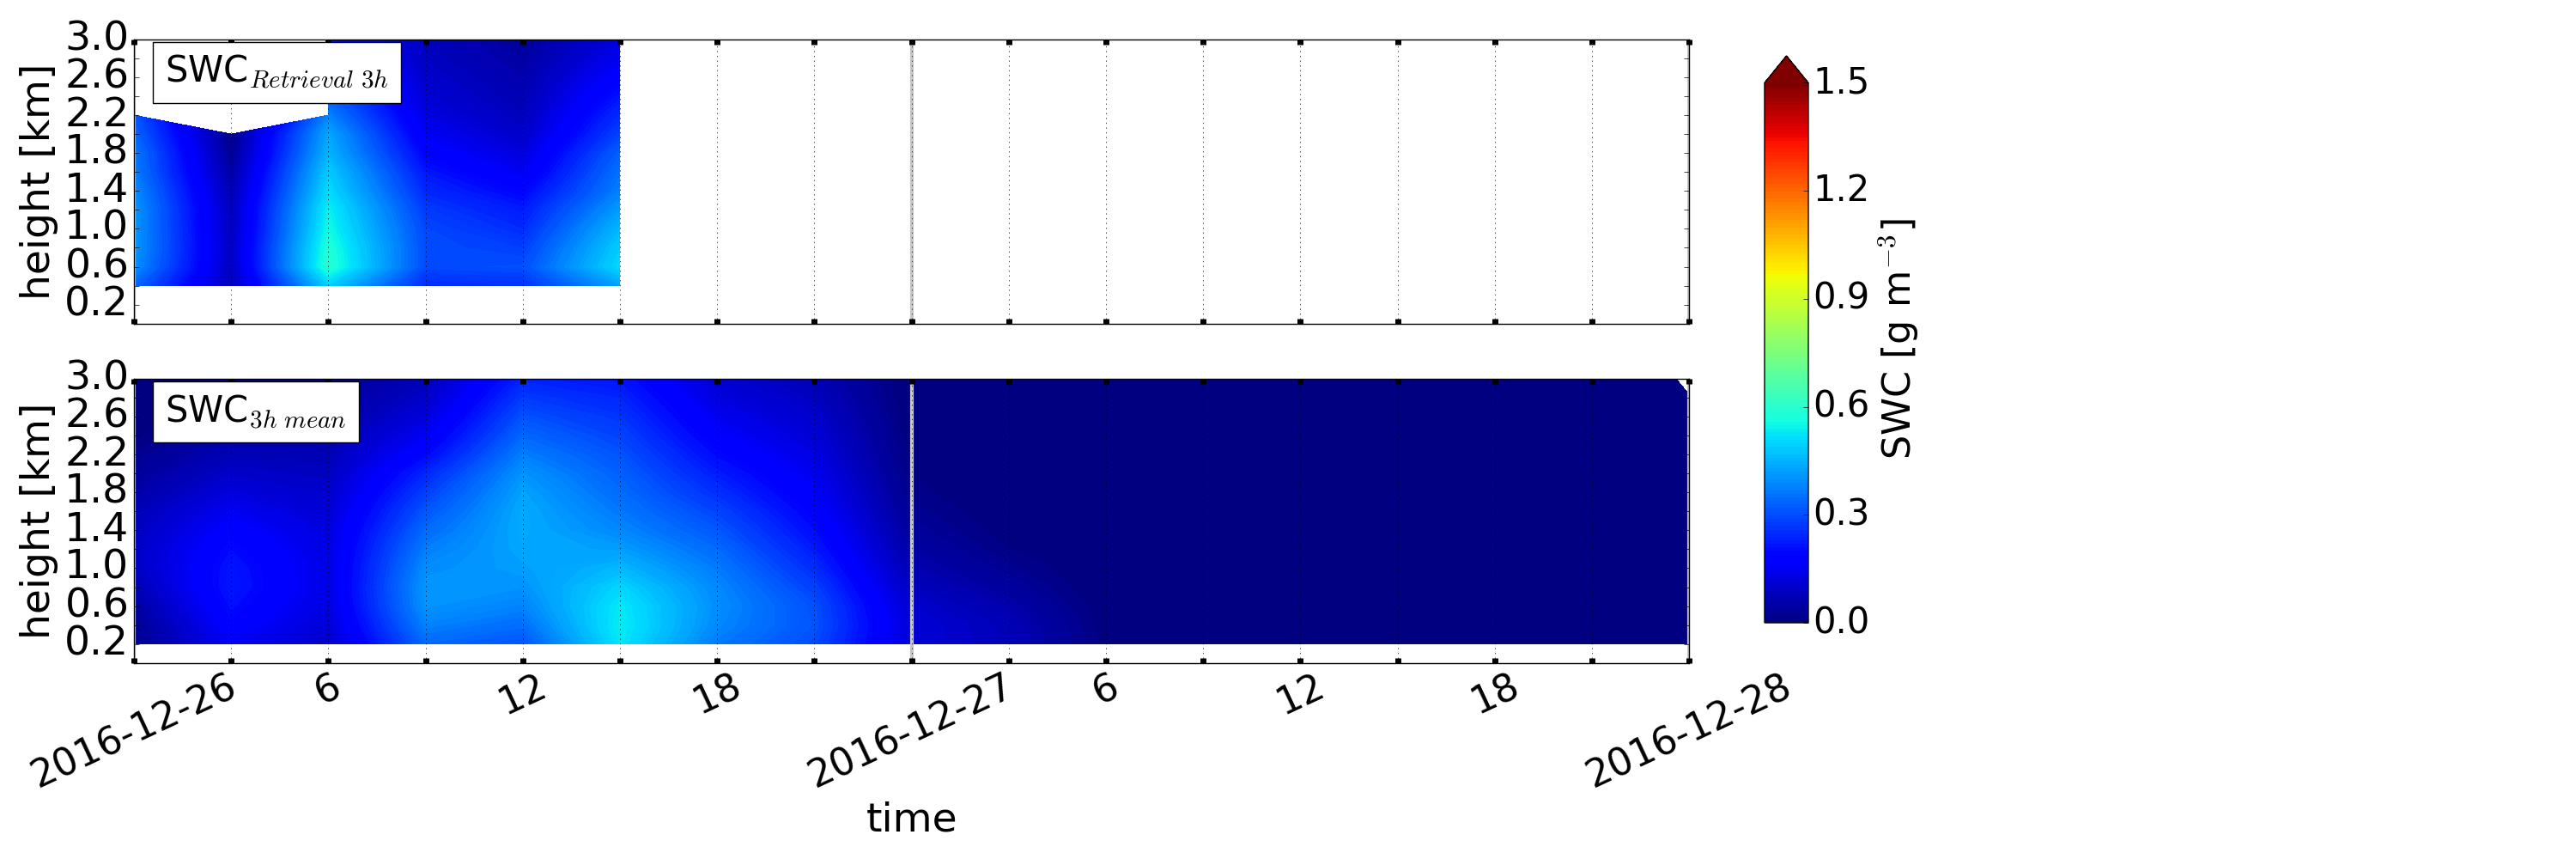
\includegraphics[trim={0.cm 0.8cm 19.cm 0.5cm},clip,width=0.9\textwidth]{./fig_vert_SWC_3h/20161226}
		\caption{}\label{fig:SWC3h:26}
	\end{subfigure}
	\caption{\textit{(As \Cref{fig:SWC21}.)} Initialisation \SI{26}{\dec} at \SI{0}{\UTC}.}\label{fig:SWC26}
\end{figure}
%%%%%%%%%%%%%%%%%%%%%%%%%%%%%%%%%%%%%%%%%%%%%%%%%%%%%%%%%%%%%%%%%%%%%%%%%
\noindent
\Cref{fig:SWC22,fig:SWC23,fig:SWC24,fig:SWC25,fig:SWC26} present the reflectivity of the MRR and the snow water content retrieved from the reflectivity as well as the \SI{48}{\hour} forecast values. Minutely MRR reflectivity and retrieved snow water content can be seen in \Cref{fig:SWC:ret_22} to \ref{fig:SWC:ret_26}. \Cref{fig:SWC_EM:22} to \ref{fig:SWC_EM:26} show in the upper panel the hourly averaged values from the retrieved SWC and in the lower panel the ensemble mean of the instantaneous forecast values every hour over all ensemble member.   
Three hourly averaged retrieved values are then presented in the upper panel of \Cref{fig:SWC3h:22} to \ref{fig:SWC3h:26}, the lower panel are the ensemble mean forecast values every three hours.
%%%% fronts upslope (23+26) %%%%
% 23/12
On \SI{23}{\dec} an occlusion passes over Haukeliseter between \SIlist{16;23}{\UTC}. The passage of the occlusion on \SI{23}{\dec} is already predicted for initialisations on \SI{22}{\dec} in \Cref{fig:SWC_EM:22}, \subref{fig:SWC3h:22}. 
% The predicted hourly and three hourly snow water content increases with shorter lead time in \Cref{fig:SWC_EM:23} and \subref{fig:SWC3h:23} after \SI{16}{\UTC}.
With shorter lead time the snow water content for hourly and three hourly ensemble means increases in \Cref{fig:SWC_EM:23} and \subref{fig:SWC3h:23} after \SI{16}{\UTC} on \SI{23}{\dec}. MEPS is able to estimate the snow water content for ensemble means of time resolutions \SI{3}{\hour} in \Cref{fig:SWC3h:22}, \ref{fig:SWC3h:23}.
\\
% 26/12
On \SI{26}{\dec}, retrieved snow water content until the passage of the occlusion is observed (\Cref{fig:res:sfc_pres26,fig:res:sfc_temp26,fig:res:sfc_wd26,fig:res:sfc_ws26,fig:res:sfc_precip26}). The average of all ensemble members (\Cref{fig:SWC_EM:26}) as well as the three-hourly instantaneous SWC (\Cref{fig:SWC3h:26}) predict the frontal transition between \SIlist{15;21}{\UTC}. Initialisations already \SI{39}{\hour} prior (\SI{25}{\dec}) simulate that intense precipitation will occur over a short time (\Cref{fig:SWC_EM:25}, \subref{fig:SWC3h:25}). 
\\
%%%%%%% image liquid forecast 25 %%%%%%%%%%%%%%%%
\begin{figure}[t]
	\centering
	\begin{subfigure}[b]{\textwidth}
		\centering
		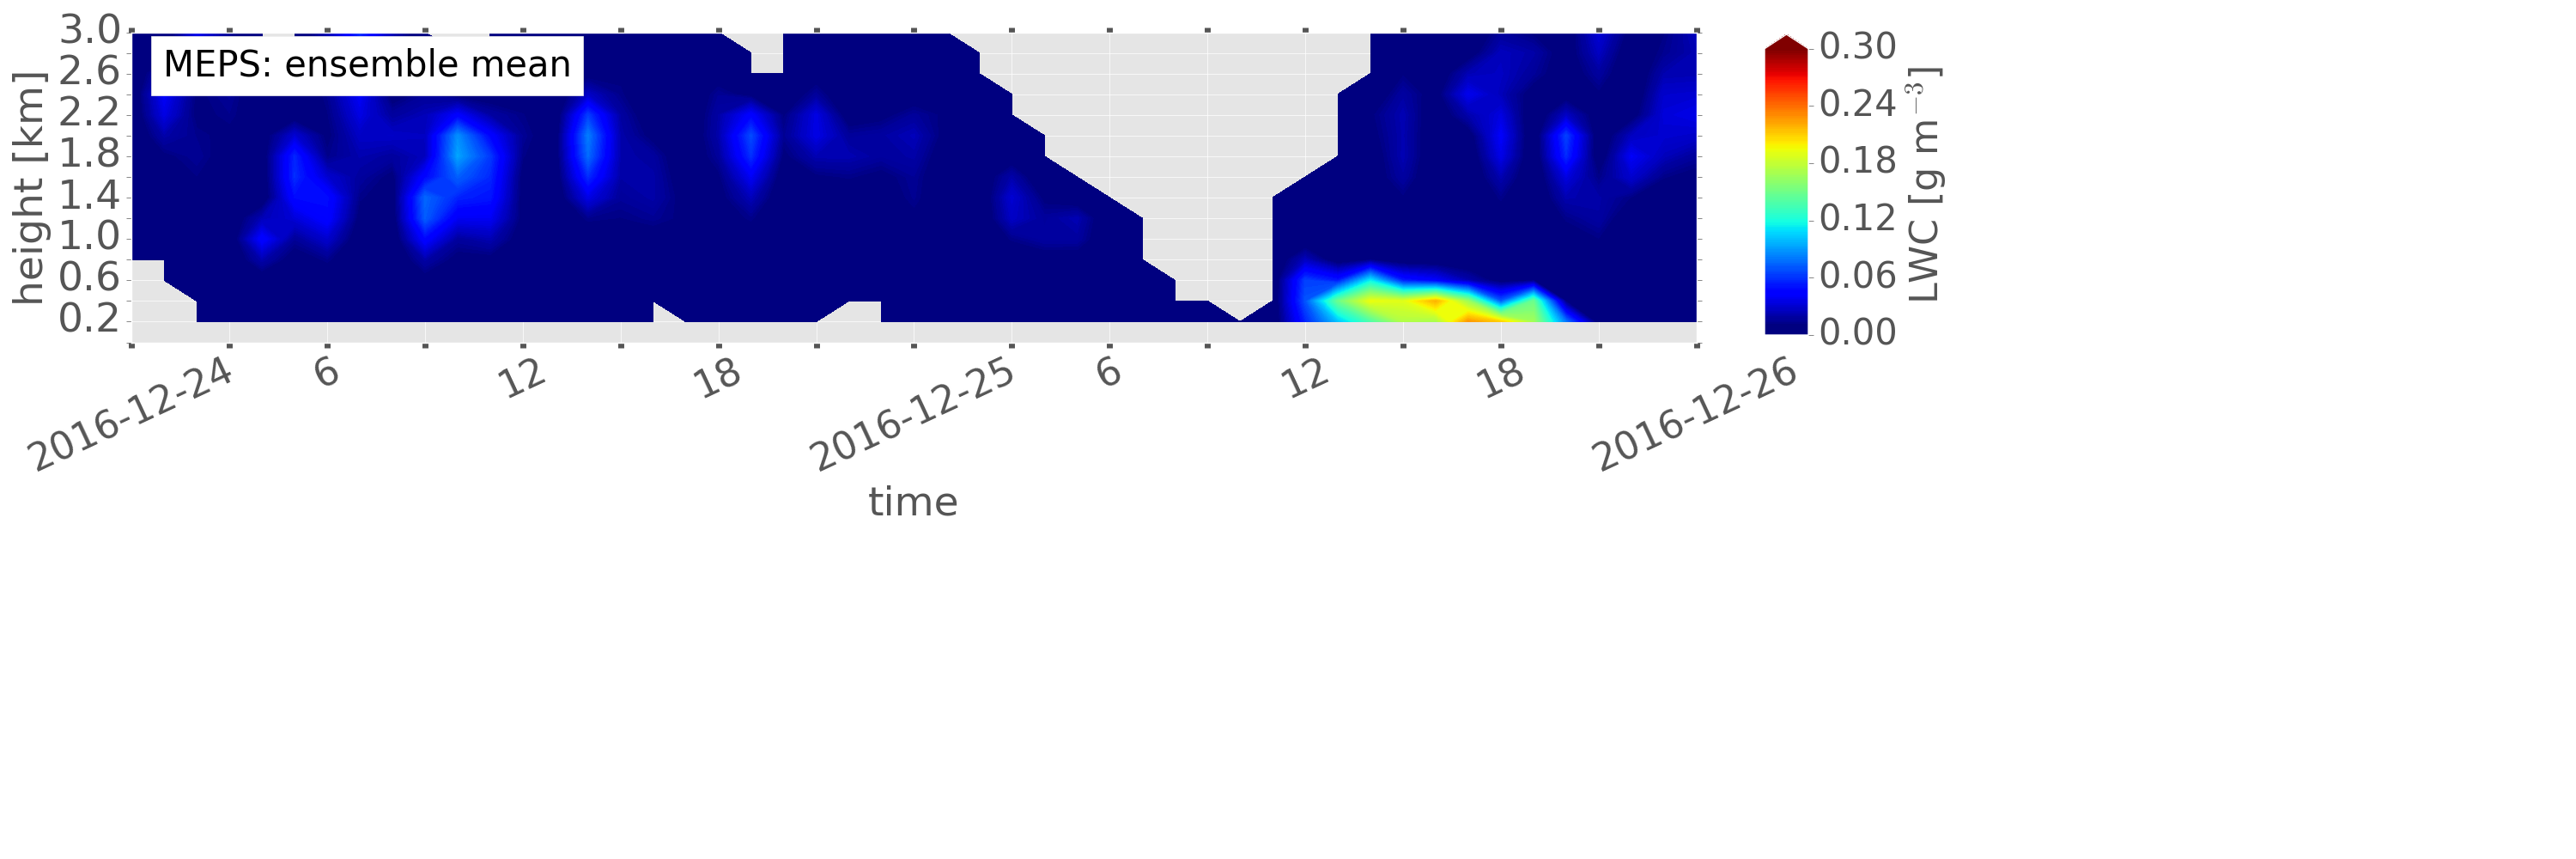
\includegraphics[trim={0.cm 11.5cm 18.5cm 0.4cm},clip,width=\textwidth]{./fig_vert_LWC_EM/20161224}
		\caption{}\label{fig:LWC:24}
	\end{subfigure}
	\begin{subfigure}[b]{\textwidth}
		\centering
		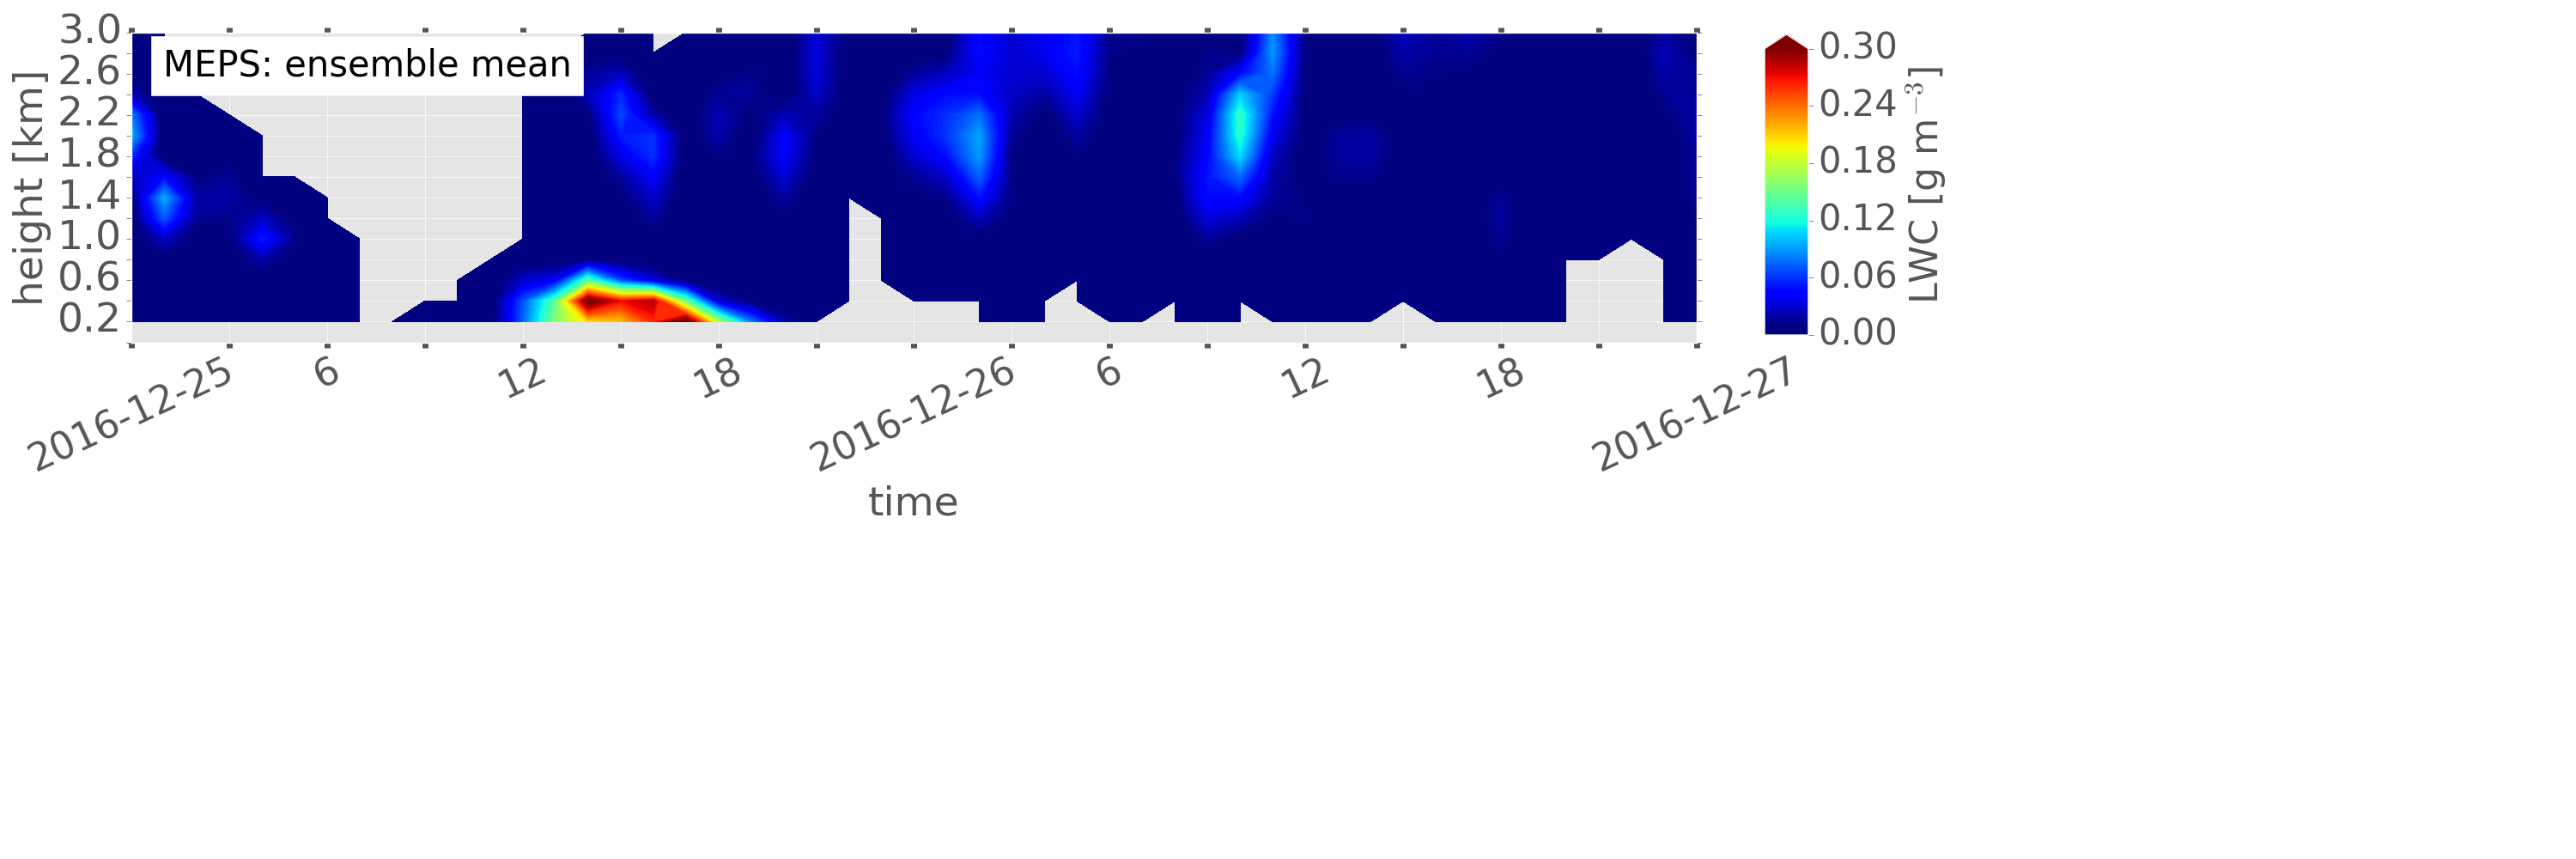
\includegraphics[trim={0.cm 10cm 18.5cm 0.4cm},clip,width=\textwidth]{./fig_vert_LWC_EM/20161225}
		\caption{}\label{fig:LWC:25}
	\end{subfigure}
	\caption{Ensemble mean \SI{48}{\hour} MEPS forecast for liquid water content. The Liquid water content is averaged over a layer thickness of \SI{200}{\metre}.  Missing values are neglected. Liquid water content according to the colour bar.
		%200m hourly averaged LWC forecast from MEPS with all ensemble members, neglecting missing values.
		Initialised on \SIlist{24;25}{\dec} at \SI{0}{\UTC}. 
	}\label{fig:LWC:2425}
\end{figure}
%%%%%%%%%%%%%%%%%%%%%%%%%%%%%%%%%%%%%%%%%%%%%%
\noindent
%%%% warm sector --> liquid (25) %%%%%
In general, the \SI{25}{\dec} %was a very weak 
storm had little snow but much %with 
liquid precipitation observed between \SIlist{11;19}{\UTC} in \Cref{fig:ret:refl25}. The retrieved snow water content in \Cref{fig:SWC24} and \ref{fig:SWC25} show a gap of missing values during liquid precipitation (\Cref{sec:pre_snow}).
The initialisations on \num{24} (\Cref{fig:SWC24}) and \SI{25}{\dec} (\Cref{fig:SWC25}) show forecasted snow water content less than \SI{0.4}{\SWC} for \SI{25}{\dec} while the retrieved maximum value is \SI{0.7}{\SWC} at \SI{15}{\UTC}.
\\
To see if liquid precipitation is predicted, the atmospheric cloud condensed water content and rainfall amount in model levels is summed (\Cref{fig:LWC:2425}). \Cref{fig:LWC:24} and \subref{fig:LWC:25} show liquid water content for initialisations on \SI{24}{\dec} and \SI{25}{\dec}, respectively. Positive \SI{2}{\metre} air temperatures are forecasted between \SIlist{12;21}{\UTC} (\Cref{fig:res:sfc_temp25}). Initialisations more than \SI{24}{\hour} prior (\SI{24}{\dec}) already show the occurrence of the liquid precipitation layer (\Cref{fig:LWC:24}). \Cref{fig:LWC:24} and \subref{fig:LWC:25} also show a narrow liquid layer thickness up to \SI{800}{\metre} for initialisations on \num{24} and \SI{25}{\dec}. 
\\
In Norwegian mountainous terrain this is an important forecast ability, since precipitation change can lead to a increased risk for people. The avalanche danger increases with the precipitation change especially during high wind speeds \citep{hansen_warmer_2014}. A change from snow to liquid precipitation increases the risk of transport accidence because of freezing rain.
Since MEPS forecasts the liquid layer correctly in thickness and duration it seems to be a good interaction between the \SI{2}{\metre} air temperature and the temperature in model levels. To produce the forecast analysis in MEPS, upper-air and surface assimilation is decoupled when starting from the model background (\Cref{sec:AROME}). MEPS \SI{2}{\metre} air temperature forecasts show the increase in temperature between \SIlist{12;18}{\UTC} on \SI{25}{\dec} (\Cref{fig:res:sfc_temp25}). This follows, that \SI{2}{\metre} air temperature is correctly translated to the upper model levels by applying a realistic temperature gradient, so that liquid precipitation is forecasted. 
The model level temperature must also reach a certain temperature threshold to forecast precipitation as liquid. 
This follows a high accuracy of MEPS for liquid forecast and the positive impact of using a high resolution convective scheme model. Precipitation is placement dependent. Lower horizontal resolution models, such as ECMWF, simulate for large grid cell area. This may lead that low temperature at a mountain top is predicted even though the meteorological observation in a valley observes rain, because an altitude difference of some hundred meter. %This can lead to forecasts of frozen precipitation instead of liquid.
%%%% turbulent (24+26) %%%%%
\\
\\
%%%% 1h average, EM01 %%%%%%%%%
The hourly ensemble mean using all ensemble members and neglecting the missing values is not a fair comparison. Therefore, an ensemble mean is created only with the deterministic and first perturbed ensemble member. Averaging only the deterministic and first perturbed ensemble member forecast leads to little snow water content (\Cref{fig:SWC1h}). \Cref{fig:SWC1h:22}, \subref{fig:SWC1h:23} and \subref{fig:SWC1h:25}, \subref{fig:SWC1h:26} show no occurrence of occlusion passages on \num{23} and \SI{26}{\dec}, respectively. Furthermore, the pulsing on \SI{24}{\dec} is seen weaker for initialisations on \SI{24}{\dec} (\Cref{fig:SWC1h:24}), but not \SI{48}{\hour} prior.
\\
A comparison with all other days show the same result, when only the deterministic forecast and first perturbed member is used \Cref{fig:SWC1h}. 
% In \Cref{fig:SWC1h:25} and \subref{fig:SWC1h:26} the amount of snow water content is very low. 
% Hourly averages, only using the deterministic forecast and the first ensemble member show no occurrence of the occlusion passages on \num{23} and \SI{26}{\dec} (\Cref{fig:SWC1h:23}, \subref{fig:SWC1h:26}).
% The deterministic forecast (EM0) and ensemble member one in \Cref{fig:EM09_22} indicate peaks of high SWC before \SI{8}{\UTC}. The retrieved SWC on \SI{23}{\dec} had two peaks, one at around \SI{2}{\UTC} and another at \SI{4}{\UTC}. 
\\
In \Cref{fig:EM09}, a comparison with each individual ensemble member shows high instantaneous values ($\ge$\SI{2.0}{\SWC}), especially for the deterministic and first ensemble member. This is seen for initialisations on almost all days during the Christmas event. 
\\
Surface overestimations is seen on \num{24}, \num{25}, and \SI{26}{\dec} (\Cref{sec:sfc_acc}). Higher predicted SWC for the deterministic and first perturbed member (\Cref{fig:EM09:24,fig:EM09:25,fig:EM09:26}) might have led to an overestimation of surface accumulation seen in \Cref{fig:sfc_acc24,fig:sfc_acc25,fig:sfc_acc26} (for ensemble member zero and one).
%High SWC is predicted by the deterministic forecast for initialisations on \num{24}, \num{25}, and \SI{26}{\dec} than for any other ensemble member (\Cref{fig:EM09_24} to \subref{fig:EM09_26}). % This deviation might have led to an overestimation of surface accumulation on \num{24} (\Cref{fig:sfc_acc24}), \num{25} (\Cref{fig:sfc_acc25}), and \SI{26}{\dec} (\Cref{fig:sfc_acc26}). %, where the deterministic forecast simulates higher values than the perturbed members .  
% 
% \\
\\
\\
%%%% CV + EM09 %%%%%%%%%
The variation of each initialised ensemble member for snow water content is given in \Cref{fig:EM09} for the respective day. % %initialised on the respective day are given in \Cref{fig:EM09}.
%The snow water content forecast of all nine ensemble member is given in \Cref{fig:EM09}.
One possibility to quantify the variability of all ensemble member during the Christmas 2016 storm, is by calculating the coefficient of variation (CV) for SWC, described in \Cref{sec:ens_mean_spread}. 
\Cref{fig:vari:EM22,fig:vari:EM24,fig:vari:EM25,fig:vari:EM26} show the coefficient of variation for SWC and gives the possibility to compare the SWC for different days with each other. The interpretation of the coefficient of variation for SWC is presented in \Cref{tab:verification}.
%%% table verification %%%%%%%%%%%%%%%%%%%%%%%%%%%%%%%%%%%%%
\begin{table}[t!]
	\begin{center}
		\caption{Interpretation of the coefficient of variation for SWC.} \label{tab:verification}
		\begin{tabular}{lc|c}
			\hline\hline
			\multicolumn{2}{c|}{\textbf{Size of CV}} & {\textbf{Interpretation}} \\ 
			\multicolumn{2}{c|}{[\SI{}{\percent}]} & variability \\ \hline \hline 
			\multicolumn{2}{c|}{\numrange{0}{< 25}} & negligible  \\ \hline
			\multicolumn{2}{c|}{\numrange{25}{< 50}} & low \\ \hline
			\multicolumn{2}{c|}{\numrange{50}{< 75}} & moderate \\ \hline
			\multicolumn{2}{c|}{\numrange{75}{< 100}} & high \\ \hline
			\multicolumn{2}{c|}{\num{100} to $\infty$} & very high  \\ \hline \hline
		\end{tabular}
	\end{center}
\end{table}
%%%%%%%%%%%%%%%%%%%%%%%%%%%%%%%%%%%%%%%%%%%%%%%%%%%%%%%%%%%%%%%%%%%%%%%%%
\noindent
\\
The grey line in \Cref{fig:ens_vari} presents the ensemble mean of the hourly predicted SWC values. The darker the shading in \Cref{fig:ens_vari} the smaller the variation of the SWC relative to the mean. 
\\
MEPS data does not exist for all ten ensemble members on \SI{23}{\dec}. No coefficient of variation is calculated for this day, since only six perturbed members were available. Therefore, the initialisation on \SI{22}{\dec} is used to validate the forecast. 
%%%%%%% image variability %%%%%%%%%%%%%%%%
\begin{figure}[t!]
	\centering
	\begin{subfigure}[b]{\textwidth}
		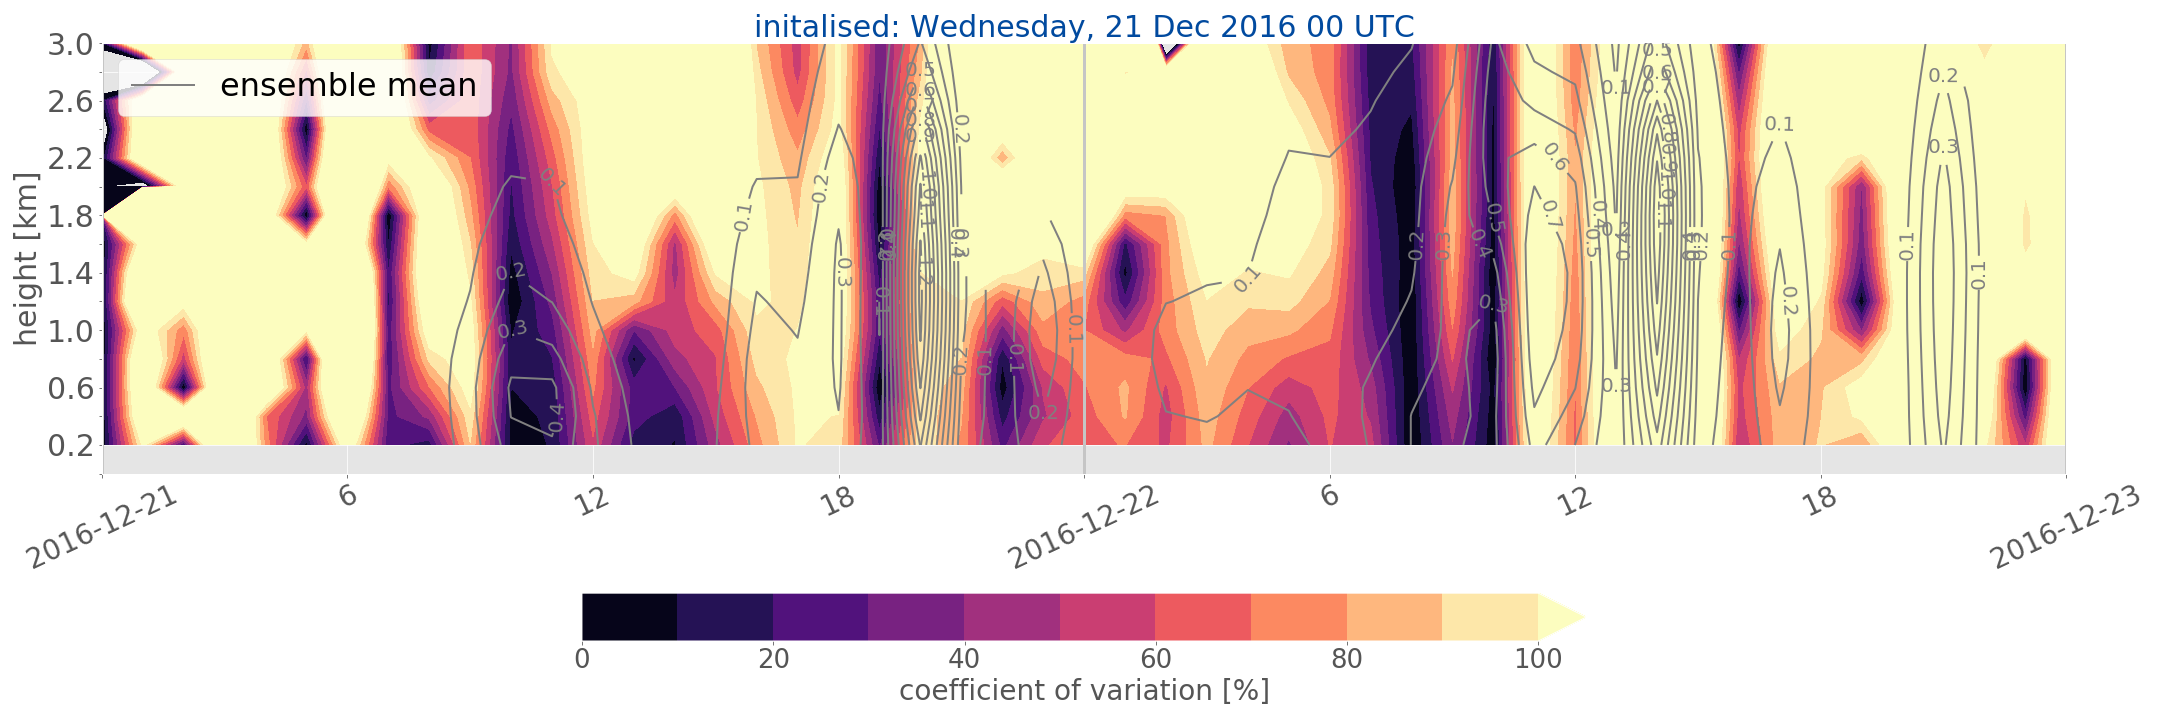
\includegraphics[trim={0cm 5cm 0cm 0cm},clip,width=\textwidth]{./fig_variation/20161221}
		\caption{}\label{fig:vari:EM21}
	\end{subfigure}
	\begin{subfigure}[b]{\textwidth}
		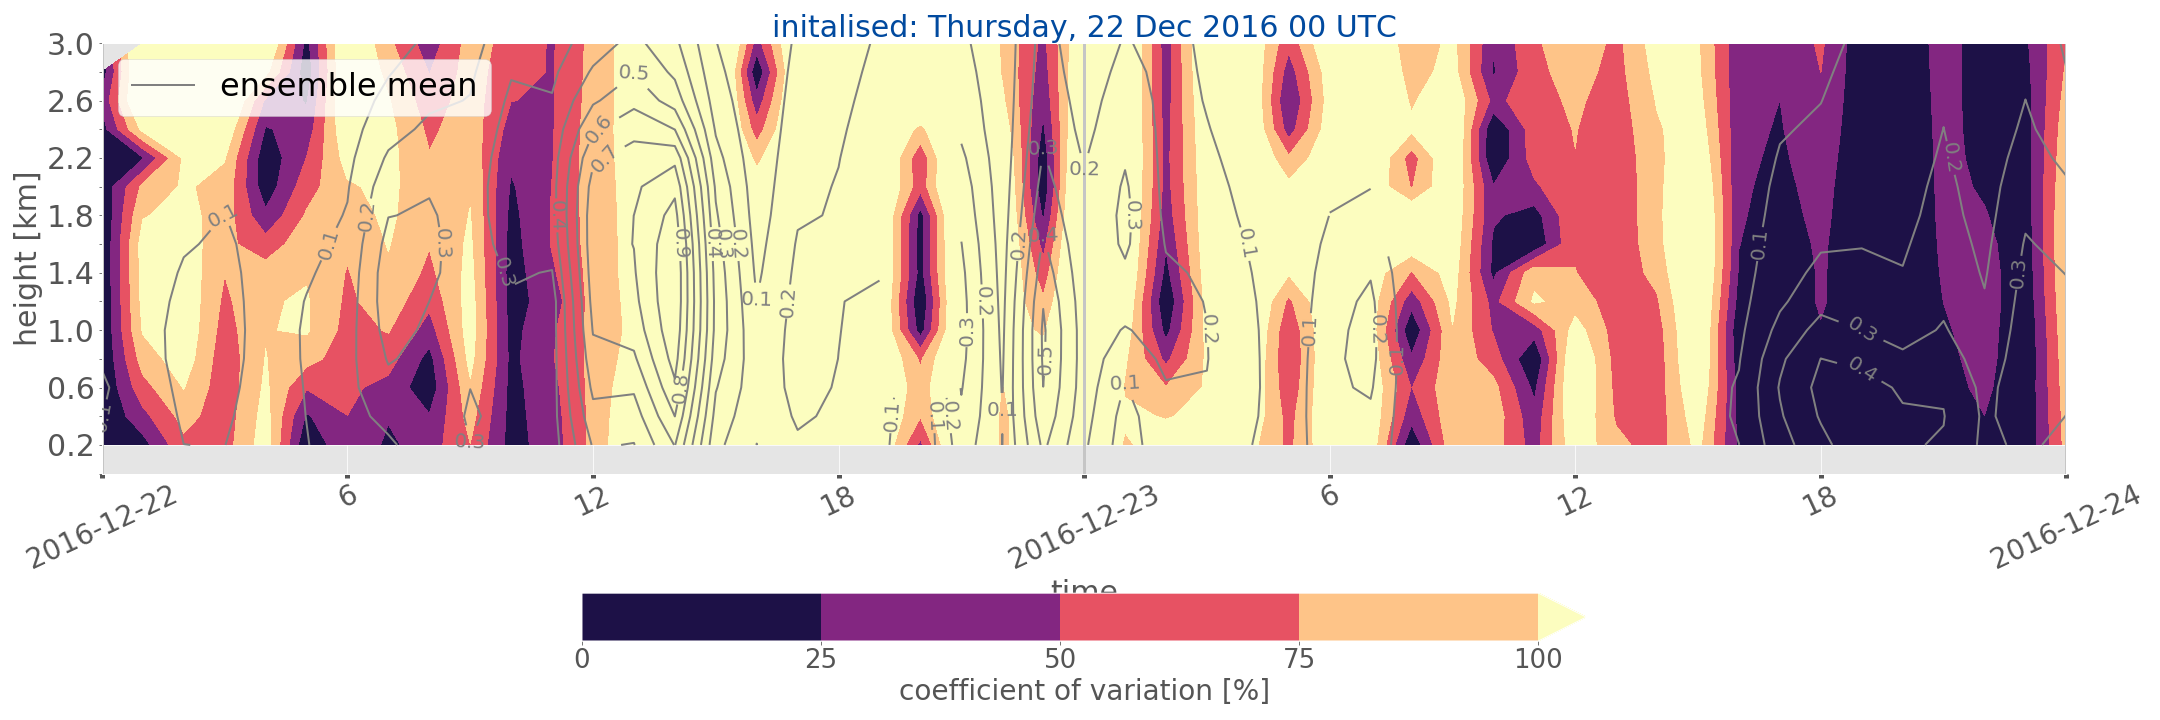
\includegraphics[trim={0cm 5cm 0cm 0cm},clip,width=\textwidth]{./fig_variation/20161222}
		\caption{}\label{fig:vari:EM22}
	\end{subfigure}
	\begin{subfigure}[b]{\textwidth}
		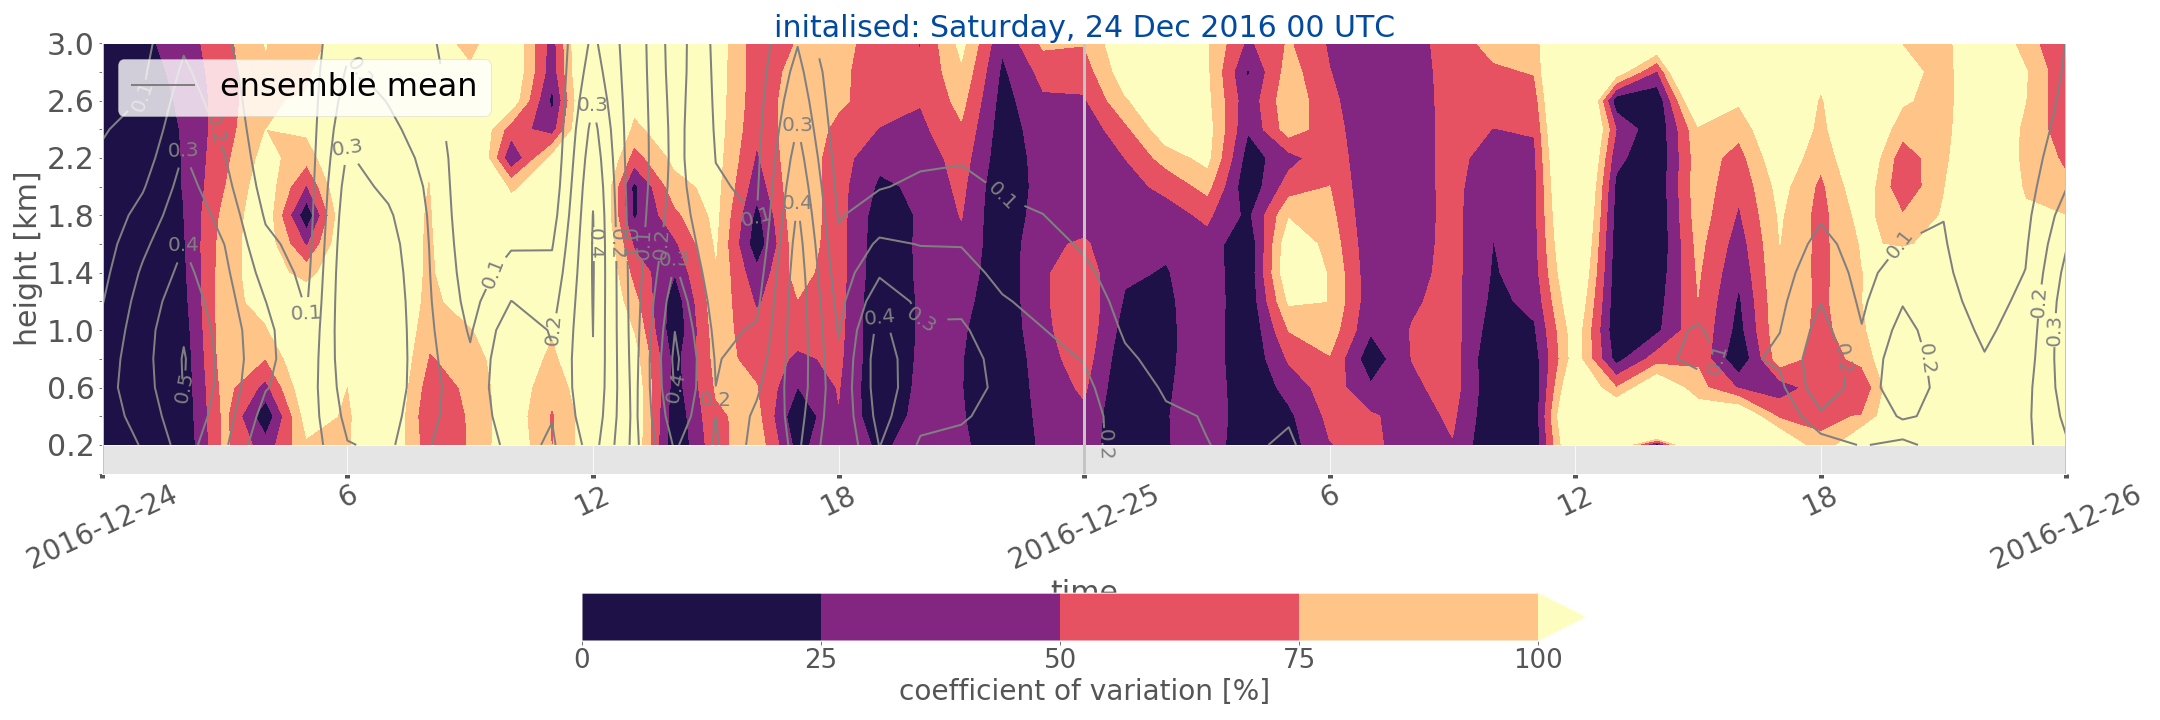
\includegraphics[trim={0cm 0cm 0cm 0cm},clip,width=\textwidth]{./fig_variation/20161224}
		\caption{}\label{fig:vari:EM24}
	\end{subfigure}
	\caption{SWC variation of the ten ensemble members of MEPS. The lighter the colour according to the colour bar the higher the variation between the perturbed ensemble members. In grey the ensemble mean of all ten members. For initialisations on \num{22} and \SI{24}{\dec}. \textit{Continued on next page.}}\label{fig:ens_vari}
\end{figure}
\begin{figure}[t!]\ContinuedFloat
	\begin{subfigure}[b]{\textwidth}
		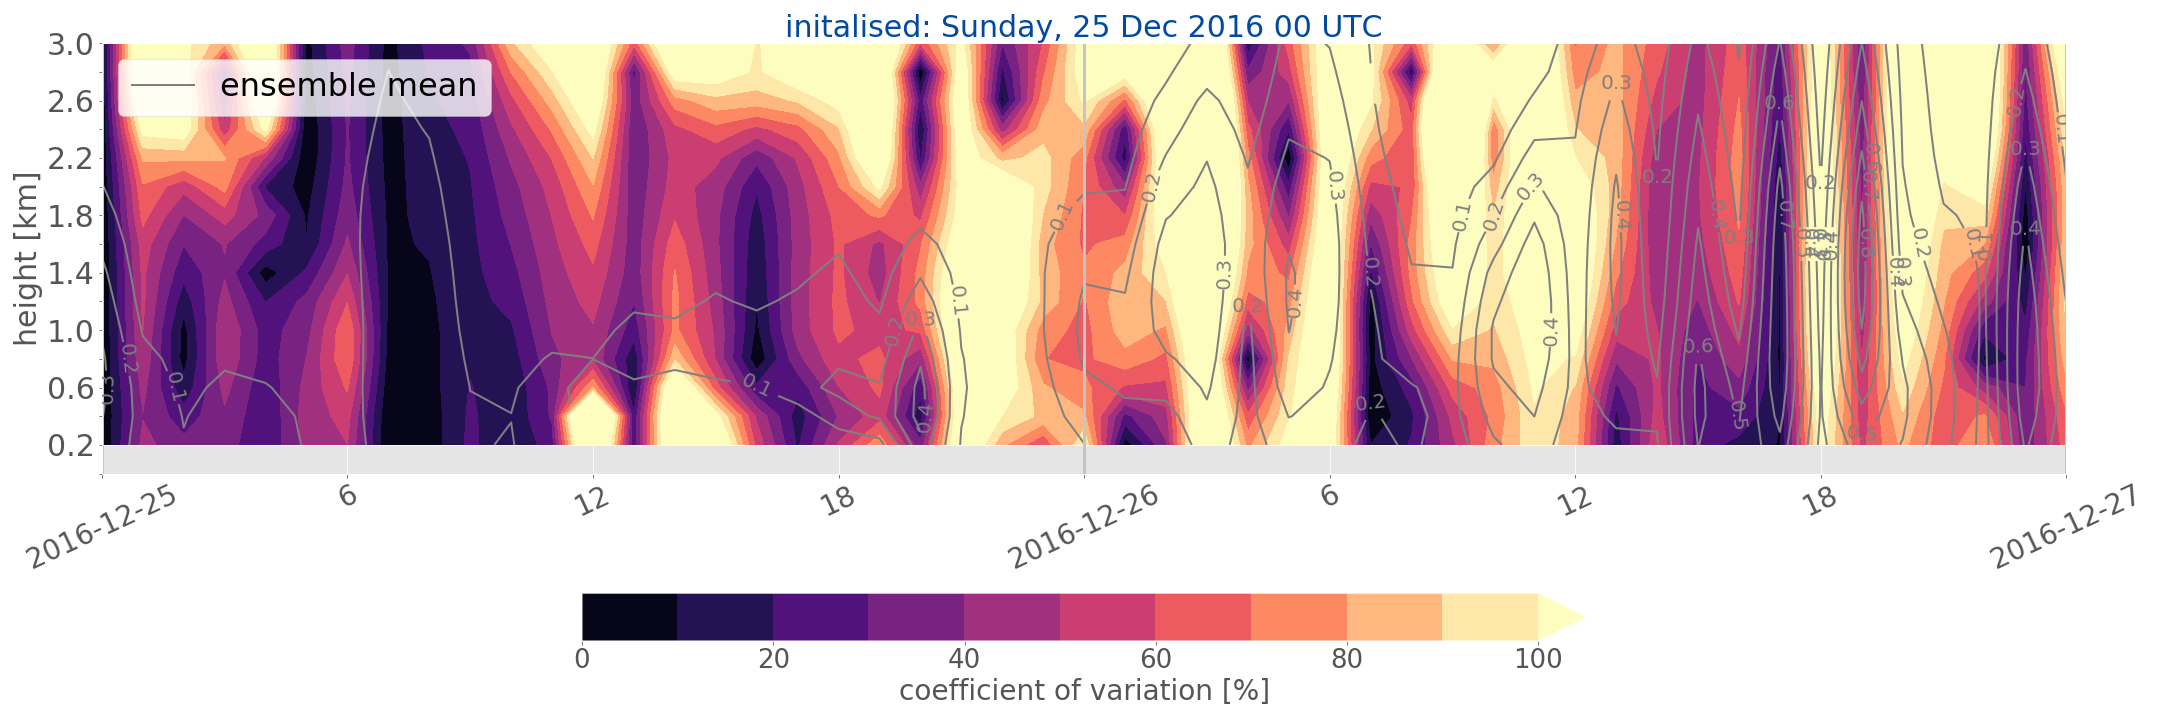
\includegraphics[trim={0cm 5cm 0cm 0cm},clip,width=\textwidth]{./fig_variation/20161225}
		\caption{}\label{fig:vari:EM25}
	\end{subfigure}
	\begin{subfigure}[b]{\textwidth}
		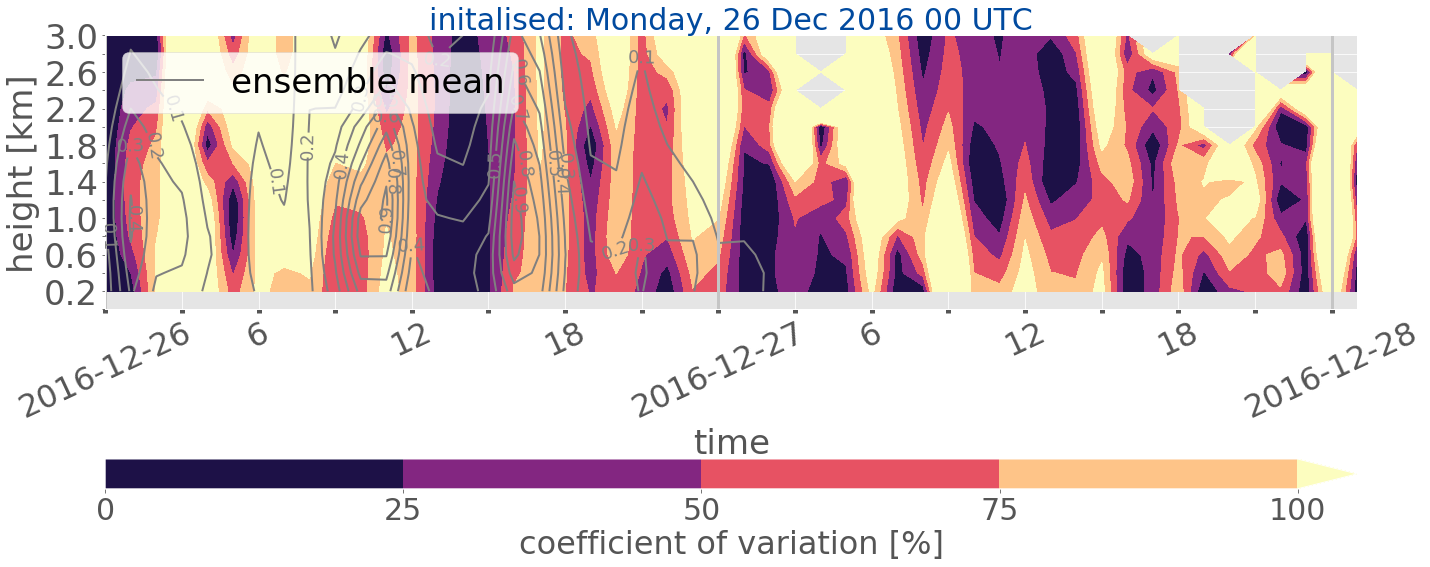
\includegraphics[trim={0cm 0cm 0cm 0cm},clip,width=\textwidth]{./fig_variation/20161226}
		\caption{}\label{fig:vari:EM26}
	\end{subfigure}
	\caption{\textit{(Continued from previous page.)} Initialisation \num{25} and \SI{26}{\dec}.}
\end{figure}
%%%%%%%%%%%%%%%%%%%%%%%%%%%%%%%%%%%%%%%%%%%%%
\noindent 
%%%% fronts upslope (23+26) %%%%
% 23/12
On \SI{23}{\dec}, two intense SWC pulses are observed in the lower troposphere at \SIlist{2;4}{\UTC} (\Cref{fig:SWC:ret_23}). The deterministic forecast, initialised on \SI{22}{\dec} predicted a pulse at \SIlist{1;3}{\UTC}, where the first perturbed ensemble member (EM1) has a strong SWC at \SI{3}{\UTC}. Initialisations \SI{24}{\hour} later show only one pulse in the deterministic forecast at \SI{2}{\UTC}.
\\
The occlusion passage on \SI{23}{\dec} is seen after \SI{16}{\UTC} in \Cref{fig:SWC23}.  
%prediction for the occlusion passage is quite weak for all ensemble members. % 
% 
% ini 22/12
Initialisations on \SI{22}{\dec} (\Cref{fig:EM09_22}) show for each ensemble member a weak predicted snow water content for the transition of the occlusion. 
% ini 23/12 
No MEPS forecast data was available for four perturbed ensemble for initialisations on \SI{23}{\dec}.
The comparison of only six ensemble members %for initialisation on \SI{23}{\dec} 
in \Cref{fig:EM09_23}, display low variability between all ensemble members during the up-slope storm. %, but not as certain as for an initialisation on \SI{22}{\dec} at \SI{0}{\UTC}. 
Nevertheless, for initialisations on \num{22} or \SI{23}{\dec} all ten ensemble members forecast the pulsing precipitation pattern to occur after \SI{16}{\UTC} (\Cref{fig:EM09_22} and \subref{fig:EM09_23}). 
%All ensemble members agree well with the development of the up-slope storm on \SI{23}{\dec} after \SI{16}{\UTC} (\Cref{fig:EM09_22}). 
For prediction initialised on \SI{22}{\dec} the verification in \Cref{fig:vari:EM22} shows little variability, below \SI{50}{\percent}, and show a good agreement on the occurrence of frozen precipitation after \SI{16}{\UTC}. 
\\
% 26/12
Before \SI{16}{\UTC} a pulsing precipitation pattern is observed in the lower \SI{3}{\km} at Haukeliseter on \SI{26}{\dec}. All ten ensemble member in \Cref{fig:EM09:25,fig:EM09:26} predict pulsing patterns. Initialisations on either \num{25} or \SI{26}{\dec} show interchangeable precipitation for the deterministic and first ensemble member similar as the retrieved snow water content (\Cref{fig:SWC26}). 
\\
% occlusion
The surface observations for \SI{26}{\dec} indicate the passage of the occlusion at Haukeliseter between \SIlist{15;19}{\UTC} (\Cref{fig:obs_meps:26}). A larger variability between the ensemble members than for the occlusion passage on \SI{23}{\dec} (\Cref{fig:vari:EM22})  is shown for the evolution of the occlusion on \SI{26}{\dec} in \Cref{fig:vari:EM25}, \subref{fig:vari:EM26}.  
\\
% ini 25
Initialisations on \SI{25}{\dec} present a lower variability for the transition of the occlusion after \SI{15}{\UTC} on \SI{26}{\dec}  (\Cref{fig:vari:EM25}) than initialisations less than \SI{24}{\hour} prior (\Cref{fig:vari:EM26}). 
Therefore, an increase of variability for shorter lead time is given in \Cref{fig:vari:EM26}. %rather than long lead time (\SI{48}{\hour}). 
The variation of all members for initialisations on \SI{25}{\dec} (\Cref{fig:EM09_25}) and on \SI{26}{\dec} (\ref{fig:EM09_26}) indicate that almost all perturbed member would have predicted the precipitation after \SI{16}{\UTC} on \SI{26}{\dec}, but the ensemble mean (\Cref{fig:SWC25}, \subref{fig:SWC26}) weakens the result. 
\\
% pulsing after occlusion
Initialisations on \SI{25}{\dec} (\Cref{fig:SWC_EM:25}, \subref{fig:SWC3h:25}) show a continued pulsing precipitation pattern after the occlusion passage. The two pulses around \SI{18}{\UTC} (\Cref{fig:SWC_EM:25}) are predicted with a negligible and moderate variability in \Cref{fig:ens_vari25}. %The SWC peaks at around \SIlist{3;5}{\UTC} show a very high variability. \Cref{fig:EM09_25} displays that four out of ten ensemble members would agree with the peaked event around \SI{5}{\UTC}. Whereas the peak at \SI{3}{\UTC} is dominated by the strong predicted SWC of the deterministic forecast, which follows the high variation in \Cref{fig:vari:EM25}. 
The retrieved snow water content in \Cref{fig:SWC_EM:26} shows a pulse at \SI{1}{\UTC}.
Initialisation on \SI{26}{\dec} forecast a high snow water content around \SI{1}{\UTC} as well. The forecasted SWC pulse at \SI{1}{\UTC} is related to a moderate variability of the ensemble members (\Cref{fig:vari:EM26}). 
Initialisations on \num{25} and \SI{26}{\dec} show high forecast variability for the predicted SWC between \SIlist{9;12}{\UTC}. The peak between \SIlist{15;18}{\UTC} has a low to moderate variability between the members. When looking at \Cref{fig:EM09_26} might this disagreement be related to the variation of the vertical predicted SWC. There seems to be no agreement between the different members about the incidence of the different SWC pulses on \SI{26}{\dec}. The high conflict for the CV before noon is most likely related to the high SWC of the deterministic SWC.
\\
%%%% warm sector --> liquid (25) %%%%%
On \SI{25}{\dec} forecasts for the warm sector passage show liquid precipitation (\Cref{fig:LWC:2425}).
%
Initialisations on \SI{24}{\dec}, indicate very low forecast variability up to \SI{0.8}{\km} until noon, this is when liquid precipitation was forecasted by MEPS and observed (\Cref{fig:res:obs_masc}).
%As \Cref{fig:vari:EM24} indicates the forecast variability is very low up to \SI{1.8}{\km} until noon, this is when liquid precipitation was measured. 
The depth of the liquid layer is up to \SI{0.8}{\km} in \Cref{fig:LWC:24} and \ref{fig:LWC:25}. 
\Cref{fig:vari:EM24} and \ref{fig:vari:EM25} show the variation for SWC on \SI{25}{\dec}. Between \SIlist{12;18}{\UTC} the variation is large below \SI{0.8}{\km}. This is related to the ten ensemble members in \Cref{fig:EM09}. Each ensemble member shows between \SIlist{12;18}{\UTC} little SWC. This little snow water content leads to a higher coefficient of variation and displays as a high variability although all ensemble members agree on the timing of liquid precipitation.
%The variation coefficient for snow water content (\Cref{fig:vari:EM24} and \ref{fig:vari:EM25}) has a large disagreement below \SI{0.8}{\km}, because of a low predicted SWC in \Cref{fig:SWC24}, \subref{fig:SWC25}.
%, but 
Above \SI{0.8}{\km} the variability for snow water content between the members is low. Initialisation on \SI{24}{\dec} show low snow water content pulses in \Cref{fig:SWC_EM:24} and \subref{fig:SWC3h:24} at \SI{18}{\UTC}, which had a moderate variability (\Cref{tab:verification}, \Cref{fig:vari:EM24}). Afterwards it is very high. For the initialisation on \SI{25}{\dec} show low forecast variability until noon (\Cref{fig:vari:EM25}). While liquid precipitation is predicted the variability in the lower layer of the troposphere is first very high and shortly before \SI{18}{\UTC} not existing. A high agreement for the SWC pulse at \SI{20}{\UTC} up to \SI{0.8}{\km} exists in \Cref{fig:vari:EM25} and decreases to be moderate above.
%%%% turbulent (24+26) %%%%%
Pulsing snow water content patterns are seen for the individual ensemble member forecasts for initialisations on \SI{24}{\dec} (\Cref{fig:EM09:24}). On \SI{24}{\dec} the observed snow water content in the lower troposphere changed between intense and less intense (\Cref{fig:SWC24}).
\\
%Again, t
Comparing hourly instantaneous SWC is not a fair comparison, since there might be a time delay of half an hour about the timing of a pulse which would follow it is not seen in the hourly model forecast. Furthermore, the best agreement is reached for ensemble means of all ten ensemble member at every hour, which smear out the snow amount in the lower \SI{3}{\km}.
%This is not a fair comparison since hourly instantaneous values are used and 
%there might be a time delay of half an hour about the development of boundaries which would follow it is not seen in the model forecast. As well as the best agreement is reached for ensemble means of all ten ensemble member at every hour.
\\
\\
%%%% general weak SWC %%%%%%%%%
%%%%%%% low predicted SWC %%%%%%%%%%%%%%%%
\begin{figure}[ht!]
	\centering
	\begin{subfigure}[b]{0.49\textwidth}
		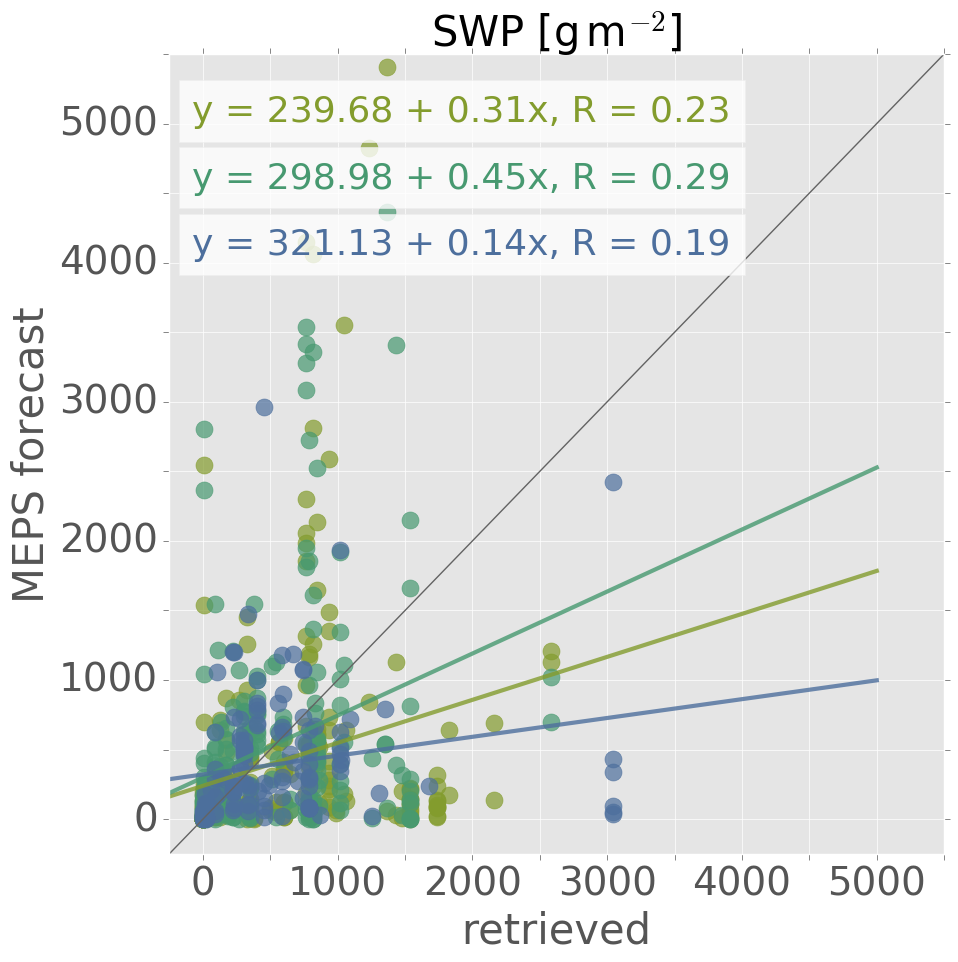
\includegraphics[width=\textwidth]{./fig_SWP_scat/EM09_20161221_23_00}
		\caption{}\label{fig:SWP:2123}
	\end{subfigure}
	%
	\begin{subfigure}[b]{0.49\textwidth}
		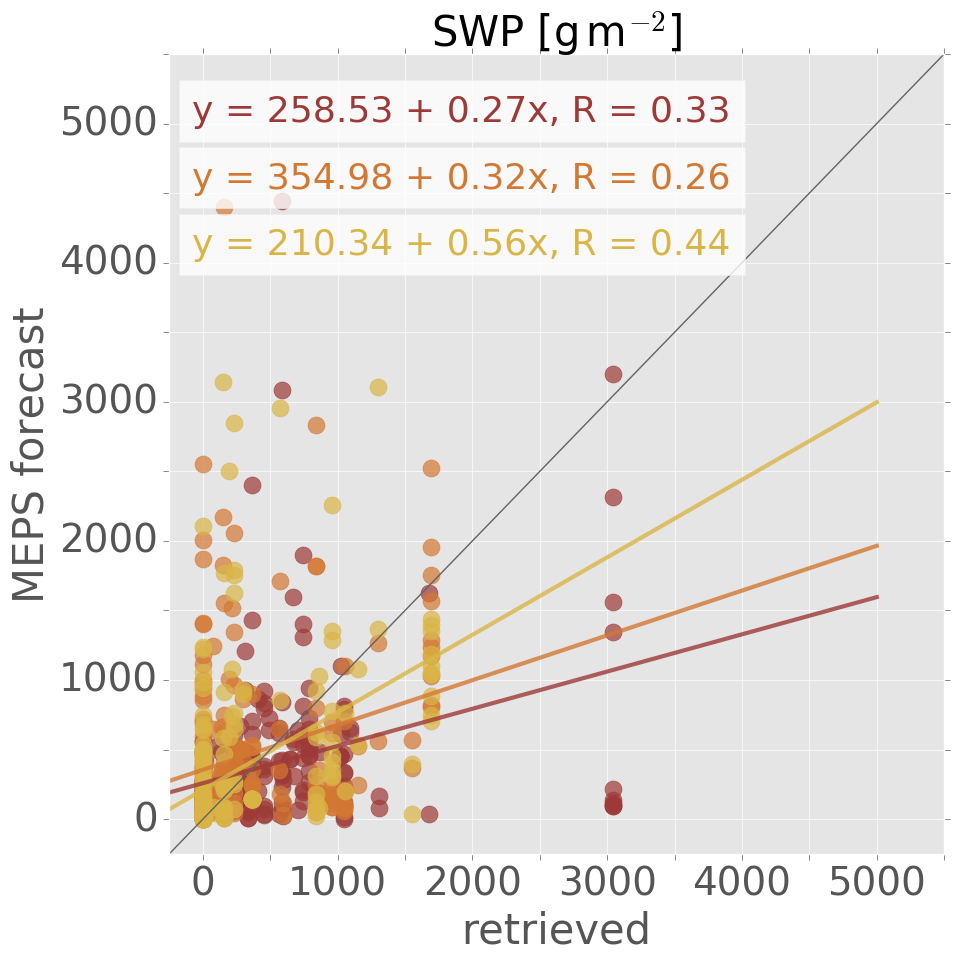
\includegraphics[width=\textwidth]{./fig_SWP_scat/EM09_20161224_26_00}
		\caption{}\label{fig:SWP:2426}
	\end{subfigure}
	% 	% label
	% 	\begin{subfigure}[b]{0.49\textwidth}
	% 		\centering
	% 		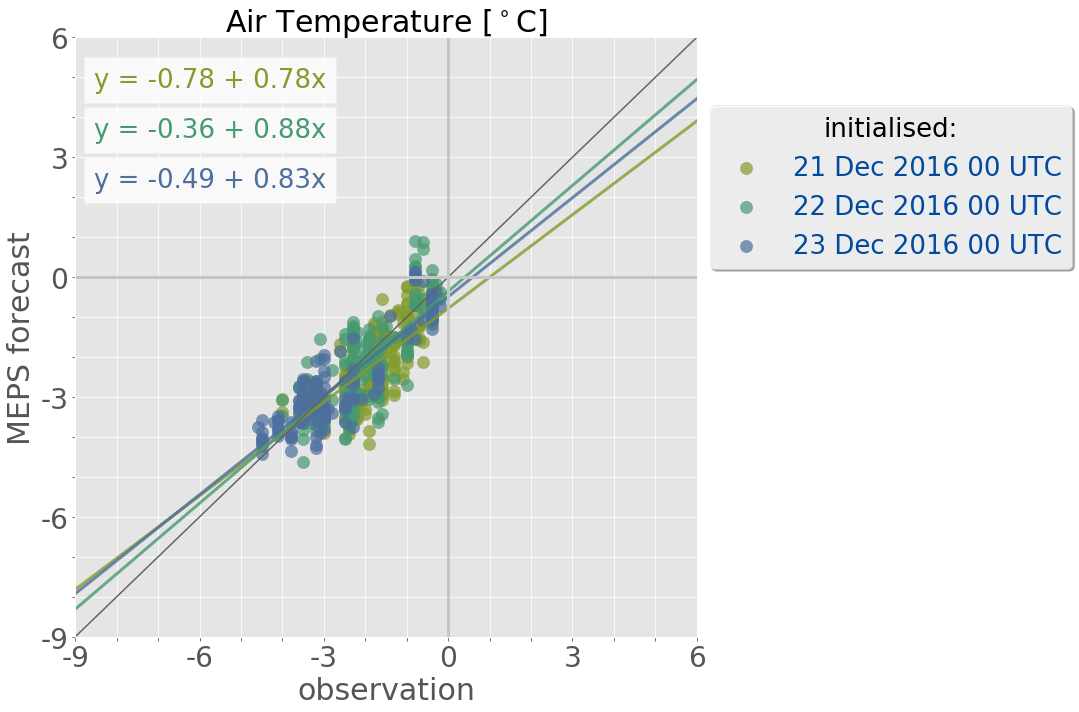
\includegraphics[trim={25.cm 15.5cm 0cm 3.6cm},clip,
	% 		width=0.8\textwidth]{./fig_sfc_temp/obs_model_20161221_23_00_label}
	% 	\end{subfigure}
	% 	\begin{subfigure}[b]{0.49\textwidth}
	% 		\centering
	% 		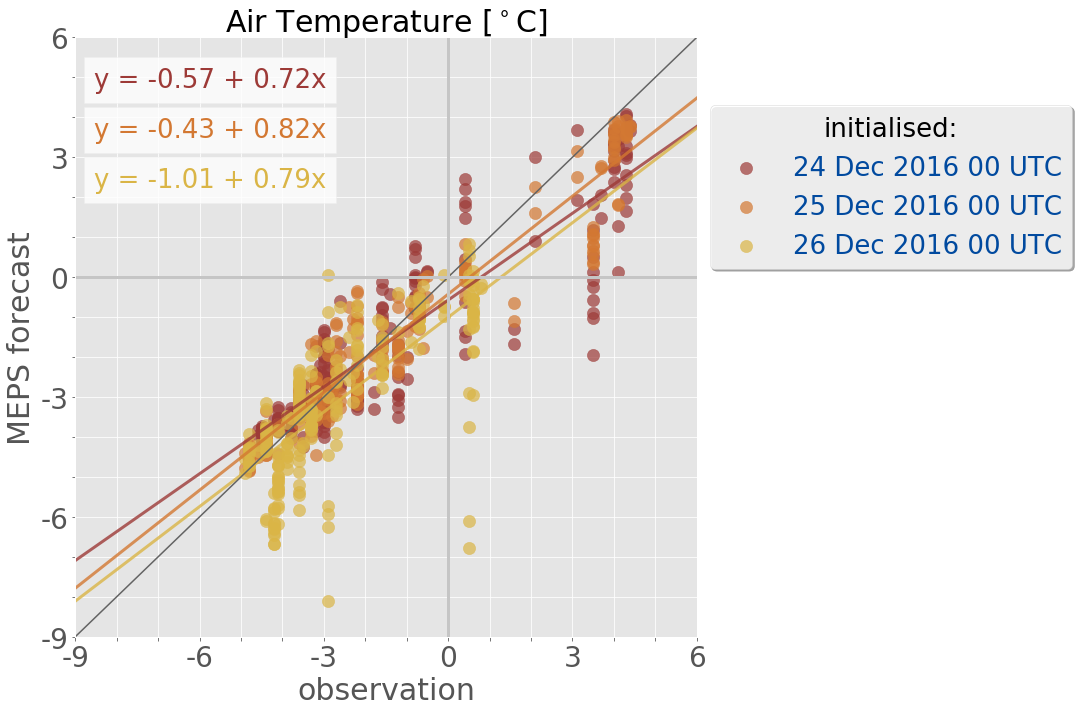
\includegraphics[trim={25.cm 15.5cm 0cm 3.6cm},clip,
	% 		width=0.8\textwidth]{./fig_sfc_temp/obs_model_20161224_26_00_label}
	% 	\end{subfigure}
	\caption{Snow water path correlation between retrieved and forecasted values for \SI{48}{\hour} lead time and all ensemble member. Separated for \num{21} to \SI{23}{\dec} (\protect\subref{fig:SWP:2123}) and \num{24} to \SI{26}{\dec} (\protect\subref{fig:SWP:2426}).}\label{fig:SWP}
\end{figure}
%%%%%%%%%%%%%%%%%%%%%%%%%%%%%%%%%%%%%%%%%%%%%%
\noindent
%In general, t
The forecasted instantaneous ensemble mean snow water content% amount 
is lower ($\le$ \SI{1.2}{\SWC}) than the retrieved values ($\le$ \SI{1.5}{\SWC}) for the 2016 Christmas storm.% on \SI{23}{\dec}. 
%Still, the instantaneous values averaged for all ensemble members are much weaker than the retrieved SWC. 
For the first glance MEPS simulates realistic snow water content when compared to observed snow water content up to \SI{3}{\km} and shows similar precipitation patterns. %Even though smeared out ensemble mean prediction occur compared to the observations. %\Cref{fig:SWC:21,fig:SWC:22,fig:SWC:23,fig:SWC:24,fig:SWC:25,fig:SWC:26} give a low forecasted ensemble mean of predicted SWC in the course of a day.
The average of all ten ensemble members leads to a smeared out ensemble mean for hourly or three hourly instantaneous values in \Cref{fig:SWC:21,fig:SWC:22,fig:SWC:23,fig:SWC:24,fig:SWC:25,fig:SWC:26}. 
To compare if lower snow water content was predicted than retrieved from the optimal estimation retrieval the snow water path is calculated (\Cref{sec:SWP}). 
\\
\Cref{fig:SWP} shows the correlation between retrieved and individual ensemble member \SI{48}{\hour} forecasts of snow water path. The slope parameter is for the days of the Christmas storm less than \SI{0.6}{\SWP} indicating a weak uphill correlation between retrieved and predicted values. %For all days, the slope of the regression line is smaller than \SI{1}{\SWP}. 
This shows, retrieved values are larger than the instantaneous ensemble member forecasts for snow water content. 
\\
On \num{24}, \num{25}, and \SI{26}{\dec} the surface snow accumulation is overestimated by MEPS (\Cref{fig:sfc_acc24,fig:sfc_acc25,fig:sfc_acc26}). This overestimation is not seen in the vertical. It might be related to the use of hourly instantaneous values in the vertical whereas the surface precipitation amount is the accumulated total precipitation at each hour. 
\\
Furthermore, it could be related to the interaction between the vertical model forecast and the surface forecast. Also, the optimal estimation retrieval fall speed is assumed to be constant (\SI{0.85}{\mPs}, \Cref{sec:ret_scheme}) whereas in MEPS the terminal speed velocity is assumed to be related to the particle diameter (\Cref{eq:fall_velo_MEPS}), which is often close to \SI{1}{\mPs} for frozen particles \citep[personal communication,][]{Priv_Comm_Jenny}. 
% Since the model estimates the wind direction correctly for west wind and local mountain effects it follows that there seems to be an interaction issue between modelled precipitation and the surface accumulation. Hourly ensemble mean of the instantaneous values could
% %Hourly vertical instantaneous values could 
% have led to a misinterpretation of the here presented results.
%\\
%Overall it seems a combination of all ten ensemble member for initialisations on \SI{22}{\dec} to be a good forecast when comparing to the retrieved SWC in \Cref{fig:SWC:ret_22}, \subref{fig:SWC_EM:22}, \ref{fig:SWC3h:22,fig:SWC:ret_23}, \ref{fig:SWC_EM:22,fig:SWC3h:22}.
% \\
% \\
% %A validation of how well the forecast performance is, is difficult to do at this stage, since the time resolution of MEPS is coarse compared to the observations. 
%  One possibility to quantify the variability of all ensemble member is by calculating the coefficient of variation (CV) for SWC, described in \Cref{sec:ens_mean_spread}. 
% \Cref{fig:vari:EM22,fig:vari:EM24,fig:vari:EM25,fig:vari:EM26} show the coefficient of variation for SWC and gives the possibility to compare the SWC for different days with each other.
\\
\\
One question to answer in this work is if the operational model MEPS simulates large scale weather systems correctly. As discussed here and in \Cref{sec:res:large_scale_sfc} it seems that the model is able to resolve the development of occlusions and warm fronts and its associated precipitation. Even with the intensification of the Christmas 2016 storm MEPS seems to be able to predict extreme events for precipitation such as occlusions and liquid precipitation related to warm sectors. %MEPS might have some issues predicting surface precipitation amount and wind speed. 
\\
MEPS also distinguishes realistically between liquid and frozen precipitation in strength and timing for the lower most atmosphere in mountainous terrain in Norway like Haukeliseter.
This can be a major challenge since a change in temperature and associated precipitation transformation can lead to high risk in the Norwegian mountains, especially during winter. 
\\
The here presented results are a first look, trying to compare a mesoscale ensemble member forecast system (MEPS) with vertical in-situ measurement for snow water content.
\\
The next section will go into detail, how the local orography at Haukeliseter may influence frozen precipitation, and how MEPS's representation of the topography may affect patterns of frozen precipitation. 
% %%%%%%%%%%%%%%%%%%%%%%%%%%%%%%%%%%%%%%%%%%%%%%%%%%%%%






%%%%%%%%% Local affects %%%%%%%%%%%%%%
\subsection{Discussion}\label{sec:res:oro_infl}
The previous chapters have indicated that the regional model MEPS is able to predict larger scale phenomena. This might be related to the outer boundary condition ECMWF or the Christmas 2016 extreme event was more predictable for large scale weather systems. In general, surface parameters such as sea level pressure and temperature were predicted well in MEPS. Only wind speed and precipitation accumulation showed overestimation in MEPS predictions. Wind speed forecasts were higher than observed wind speed. Related to the representation of the orography in MEPS the general overestimation of wind speed could already be apparent in the deterministic version AROME-MetCoOp.
\\
\\
%%%% local topography
% %%%%%%% image location %%%%%%%%%%%%%%%%
\begin{figure}[ht!]
	\begin{tabular}[t]{cc}
		\begin{tabular}[t]{c}
			\begin{subfigure}[b]{0.8\columnwidth}
				\includegraphics[trim={.3cm 2.2cm 5.5cm 2.4cm},clip,width=0.88\textwidth]{./fig_Norway/elevation_Haukeli}
				\caption{}\label{fig:res:Haukeli}
			\end{subfigure}\\
			\begin{subfigure}[b]{0.8\columnwidth}
				\includegraphics[trim={.3cm 2.2cm 5.5cm 2.4cm},clip,width=0.88\textwidth]{./fig_Norway/MEPS_elevation_Haukeli_wind}
				\caption{}\label{fig:res:MEPS_Haukeli}
			\end{subfigure}
		\end{tabular}
		&
		\begin{subfigure}[t]{0.18\columnwidth}
			\includegraphics[trim={17.5cm 2.2cm 1.8cm 2.4cm},clip,width=0.9\textwidth]{./fig_Norway/elevation_Haukeli}
		\end{subfigure}
	\end{tabular}
	\caption{Topography around Haukeliseter. In \protect\subref{fig:res:Haukeli} the DTM \SI{10}{\metre} Terrain Model (UTM33) from \cite{geonorge_dtm_2018}. Contours and shading according to the colour bar. \protect\subref{fig:res:MEPS_Haukeli}: Representation of the topography and the closest grid point to the measurement site Haukeliseter in MEPS. Contours and shading present the elevation of the grid cells. Wind barbs indicate the wind direction and speed for initialisations on \SI{23}{\dec} at \SI{0}{\UTC} after \SI{18}{\hour} lead time}\label{fig:res:topo}
\end{figure}
%%%%%%%%%%%%%%%%%%%%%%%%%%%%%%%%%%%%%%%%%%%%%%
\noindent
The Haukeliseter site is exposed to high wind speeds during the winter. The previous results in \Cref{sec:res:large_scale_sfc}, \ref{sec:sfc_acc,sec:res:large_scale_vert} have shown, that wind plays an important role for the precipitation catchment at Haukeliseter. 
\Cref{fig:res:Haukeli} presents the local topography around Haukeliseter.
The mountain plateau is surrounded by higher mountains to the west and more open to the south east (\Cref{fig:res:Haukeli}).  %this orography seems to influence the vertical precipitation pattern. 
%\Cref{fig:res:MEPS_Haukeli} shows the MEPS resolution and its \SI{2.5}{\km} grid cells around the Haukeliseter site. 
%\Cref{fig:res:topo} shows the comparison between the orography and the resolved topography by MEPS. 
\Cref{fig:res:MEPS_Haukeli} shows the \SI{2.5}{\km} grid resolution of the topography by MEPS.  
%The complex terrain represented in the model could have followed a local misplacement of a precipitation cell by a few kilometres and followed an estimation of more accumulation at the site after noon.
% \Cref{fig:res:MEPS_Haukeli} displays a high mountain to the west of the station and a small one to the south.
MEPS is able to cover some of the complex structure around the site, with the higher mountain to the west and the valley to the south-east (\Cref{fig:res:Haukeli}). Haukeliseter is at an altitude of \SI{991}{\metre} above sea level (\Cref{sec:dim:site}). In this thesis the closest grid point to the Haukeliseter measurement site is used, which is \ang{59.80}\,N, \ang{7.22}\,E (\textbf{Model} in \Cref{fig:res:MEPS_Haukeli}). The altitude of this grid point is \SI{1041}{\metre} above sea level.
\\
The elevation map in \Cref{fig:res:topo} shows, that the Haukeliseter measurement site is closer to the mountain to the west, than in reality. The valley to the south-east is shifted to north-east. 
\\
\\
%%%% general wind
%%%%%%% observed wind %%%%%%%%%%%%%%%%
\begin{figure}[ht!]
	\centering
	\includegraphics[width=0.75\textwidth]{./fig_windrose/20161221_26}
	\caption{\SI{10}{\metre} wind observed at Haukeliseter during \num{21} and \SI{26}{\dec}. Wind speed according to the colour bar.}\label{fig:windrose}
\end{figure}
%%%%%%%%%%%%%%%%%%%%%%%%%%%%%%%%%%%%%%%%%%%%%%
\noindent
\Cref{fig:windrose} shows the observed \SI{10}{\metre} wind during the 2016 Christmas storm. It shows stronger westerly winds up to \SI{20}{\mPs} at Haukeliseter. Measured south-easterlies reach wind speeds less than \SI{8}{\mPs}. \citet{wolff_new_2010} states that during precipitation events the westerly wind dominates.
\\
\\
%%%% south-west, south-east channelling
\Cref{fig:scat:wd2426} shows a good correlation for west winds, but on the other side, southerly winds seem to be troublesome to predict for MEPS. 
\Cref{fig:scat:wd2123} indicates an imbalance for south-westerly winds. While south-easterly winds (along the valley) are observed at Haukeliseter MEPS predicts the \SI{10}{\metre} wind to be south-westerly (\Cref{fig:res:topo}). 
\\
Observed south-easterly winds are channelled along the valley (\Cref{fig:res:Haukeli}). %, directed in south-east. 
% MEPS resolves it in the way that the wind is south-westerly, e.g. on \SI{23}{\dec} after \SI{18}{\hour} lead time (\Cref{fig:res:topo}). 
For large scale south-westerly flow the MEPS simulates south direction rather than 
%the observed wind direction along the 
south-easterly flow along the valley. As seen in \Cref{fig:res:topo} for \SI{23}{\dec} after \SI{18}{\hour} lead time, the wind blows along the \ang{7.2} E, since a higher (\SIrange{1500}{1650}{\metre}) elevation is to the west and a \SI{1350}{\metre} high mountain to the east.
% The \SI{10}{\metre} wind %predicted by MEPS 
% is predicted to blow between the high mountain to the west and the small mountain to the south %two elevations 
% in MEPS.
\\
On \num{21} and \SI{23}{\dec} wind directions from the south-east (\Cref{fig:res:sfc_wd21}) and south (\subref{fig:res:sfc_wd23}) were observed, respectively.
\\
As earlier discussed in \Cref{sec:res:large_scale_sfc} and \ref{sec:res:large_scale_vert}, the wind change is associated with the occlusion passage on \SI{23}{\dec} (\Cref{fig:weather:23}).
\\
%% 21/12
The wind direction change on \SI{21}{\dec} in \Cref{fig:res:sfc_wd21} is related to the large scale synoptic flow but is not associated to a frontal boundary (\Cref{fig:weather:21}). A comparison with the available large scale weather analysis map from ECMWF (\Cref{sec:largeScale}), shows that the large scale surface wind is from the south-west at \SI{6}{\UTC} on \SI{21}{\dec} (\Cref{fig:GP21_06}) and has changed to west at \SI{12}{\UTC} (\Cref{fig:GP21}). The observations at the Haukeliseter site show between \SIlist{6;12}{\UTC} wind from south-east, while the predicted MEPS wind direction is from south in \Cref{fig:res:sfc_wd21}. 
\\
The forecast model seems to forecast the wind direction overall well, only on \SI{21}{\dec} before \SI{10}{\UTC} a south-west instead of a south-east wind is predicted by MEPS (\Cref{fig:res:sfc_wd21}). It displays even if the large scale wind is from the south-west (\Cref{fig:GP21}) the local wind is rather from the south or south-east (\Cref{fig:res:sfc_wd21}). This small scale effect is most likely associated to the topography around Haukeliseter (\Cref{fig:res:topo}).
\\
\\
%%%% precip pattern
% continuous, pulsing
The orography influences the vertical precipitation pattern. A continuous structure is seen when the wind is south-easterly (up-slope) e.g. on \num{21} between \SIlist{9;12}{\UTC} (\Cref{fig:SWC21}) or \SI{23}{\dec} after \SI{15}{\UTC} (\Cref{fig:SWC23}). Westerlies produce disturbed, pulsing patterns with change between intense and less intense snow water content e.g. \SI{24}{\dec} (\Cref{fig:SWC24}). As the precipitation profiles in \Cref{fig:SWC21,fig:SWC22,fig:SWC23,fig:SWC24,fig:SWC25,fig:SWC26}\subref{fig:SWC:ret_22} show, are westerlies associated with high snow water content. In comparison continuous precipitation patterns related to south-easterlies have less intense snow water content.
\\
%% both vari
The ensemble variability in \Cref{fig:ens_vari} shows that the ensemble members are divided between the existence of the exact precipitation pulsing. 
The variability between the ensemble members for snow water content is smaller ($\le$ \SI{25}{\percent}) for precipitation related to south-easterly winds (\Cref{fig:ens_vari}). 
\\
%% continuous
The local wind direction influenced the precipitation pattern in the vertical on \num{21} and \SI{23}{\dec}. On both days, weak, south-easterly wind is observed and predicted and led to a continuous precipitation pattern between \SIlist{9;12}{\UTC} on \num{21} (\Cref{fig:SWC21}) and after\SI{15}{\UTC} on \SI{23}{\dec} (\Cref{fig:SWC23}). The precipitation is not as intense than for more turbulent precipitation structure e.g. after \SI{15}{\UTC} on \SI{21}{\dec} (\Cref{fig:SWC:ret_21}).
As \Cref{fig:SWC21,fig:SWC22,fig:SWC23} indicates the model is able to cover almost the exact timing of the up-slope storm pattern on \num{21} and \SI{23}{\dec}. The variability of each ensemble member initialised on \SI{21}{\dec} is presented in \Cref{fig:EM09_21}. It shows that almost all ensemble members agree on the occurrence of the storm pattern during \SIrange{9}{12}{\UTC}. The same is valid for the initialisations on \num{22} and \SI{23}{\dec} for the occlusion passage after \SI{15}{\UTC}.
%% pulsing
\\
Both days (\num{21} and \SI{23}{\dec}) show a moderate precipitation with not as intense snow water content than for precipitation patterns associated with westerlies such as on \SI{24}{\dec} (\Cref{fig:SWC24}). 
High wind speeds from the west and therefore over high mountains (\SI{1500}{\metre}) followed a pulsing storm pattern with alternating high and low SWC (e.g. \num{22} and \SI{24}{\dec}, \Cref{fig:SWC22} and \ref{fig:SWC24}). MEPS is able to forecast the pulsing pattern for initialisations longer than \SI{24}{\hour} prior.
%Wind from the west and therefore over high mountains (\SI{1500}{\metre}) always follow a pulsing with more intense vertical precipitation e.g. on \SI{24}{\dec}, (\Cref{fig:SWC:ret_24} and \ref{fig:SWC:ret_25}). 
This effect might be related to mountain lee wave breaking %at the mountain 
and result into a turbulent precipitation pattern with pulses of \SI{30}{\minute} intense precipitation. More precipitation events need to be studied to understand this effect around the Haukeliseter site. MEPS does not cover all pulses related to west wind during the course of a day. This is related to the short occurrence of the pulses as well as to the time resolution of MEPS. %the forecast values. 
Since the prediction values exist only every hour the model might miss some of the intense, \SI{30}{\minute} precipitation. %before or after the frozen precipitation. 
\\
\\
%%% overestimation wind speed
As \Cref{fig:scat:ws2123} and \subref{fig:scat:ws2426} present the correlation between observation and forecasts is low for high wind speeds. \Cref{fig:wind_precip} shows the relation of precipitation amount to wind direction (\ref{fig:wind_precip:WD}) and wind speed (\ref{fig:wind_precip:WS}).
While the wind direction of MEPS has a good agreement, at least for west wind, the wind speed shows larger values over all days (\Cref{fig:wind_precip}).
%The correlation between observations and forecast show an overestimation of predicted wind speed throughout the event. % \textcolor{red}{Is this overestimation different for different wind directions?} %
\citet{muller_arome-metcoop:_2017} already mentioned the bias of too strong wind speed prediction in AROME-MetCoOp.%, the previous operational deterministic version of MEPS.
% Although MEPS includes ten perturbed ensemble members, % the insufficiency of 
% the too high wind speed forecasts in AROME-MetCoOp is not resolved in extreme situations. 
\\
The surface precipitation amount show \SI{48}{\hour} accumulation only up to \SI{50}{\mm}, whereas the model predicts higher surface precipitation amount. The regression between precipitation amount and wind direction shows to be almost the same for observations and MEPS simulations. Weaker \SI{10}{\metre} wind speeds are observed than predicted. 
\\
High wind speeds might be related to the higher model grid point (\SI{1041}{\metre} above sea level) than the Haukeliseter measurement site (\SI{991}{\metre} above sea level). A difference of \SI{50}{\metre} in altitude may lead to the simulation of too high wind speeds. As earlier discussed is the double fence affected by wind (\Cref{sec:sfc_acc}). 
%%%%%%% precip WS, WD correlation %%%%%%%%%%%%%%%%
\begin{figure}
	\centering
	\begin{subfigure}[b]{0.8\textwidth}
		\centering
		\includegraphics[width=\textwidth]{./fig_scat_PP/precip_vs_WD}
		\caption{}\label{fig:wind_precip:WD}
	\end{subfigure}
	\begin{subfigure}[b]{0.8\textwidth}
		\centering
		\includegraphics[width=\textwidth]{./fig_scat_PP/precip_vs_WS}
		\caption{}\label{fig:wind_precip:WS}
	\end{subfigure}
	\caption{Correlation between surface precipitation amount accumulated over \SI{48}{\hour} and \protect\subref{fig:wind_precip:WD}, \SI{10}{\meter} wind direction, and \protect\subref{fig:wind_precip_WS}, \SI{10}{\metre} wind speed. Red indicating the observations by the double fence and weather mast. Black, the deterministic MEPS forecast and grey, the perturbed ensemble member. The regression line for each correlation and its associated regression coefficient.}\label{fig:wind_precip}
\end{figure}
%%%%%%%%%%%%%%%%%%%%%%%%%%%%%%%%%%%%%%%%%%%%%%
\noindent
%%%  overestimation sfc
\Cref{sec:sfc_acc} describes the overestimation of surface snow accumulation during the intensification of the extreme storm. MEPS forecast in \Cref{fig:sfc_acc24,fig:sfc_acc25,fig:sfc_acc26} show more ground accumulation than observed for \num{24} to \SI{26}{\dec}. Aim of this thesis is to analyse if the wind might have had an influence on the surface measurement of the double fence, which could not be shown, even if \SI{10}{\percent} under-catch by the double fence gauge is assumed (\Cref{tab:res:MEPS_err_10}).
\\
During \num{24} to \SI{26}{\dec} the wind is constantly from the west with higher wind speeds observed (\Cref{fig:obs_meps:24}, \ref{fig:obs_meps:26}) than during \num{21} to \SI{23}{\dec} (\Cref{fig:obs_meps:21}, \ref{fig:obs_meps:23}). \Cref{fig:scat:wd2123} and \subref{fig:scat:wd2426} indicate a better correlation for the observed and forecasted wind directions when precipitation overestimation occurred (\num{24} to \SI{26}{\dec}). During \num{24} and \SI{26}{\dec}, observed wind speeds were higher, up to \SI{20}{\mPs}, than on the previous days.
\\
A comparison of the hourly values of MEPS (\Cref{fig:EM09}), show neither on \num{24}, \num{25}, and \SI{26}{\dec} high snow amounts up to \SI{3}{\km} compared to the estimated SWC (\Cref{fig:SWC24,fig:SWC25,fig:SWC26}). \Cref{fig:EM09} shows values of very high instantaneous snow water content for individual ensemble members, but no prominent sign of overestimation when the surface %overestimation is present. 
simulated too much surface precipitation amount.
\\
The complex terrain and its representation in MEPS might have led to the overestimation of surface precipitation amount between \num{24} and \SI{26}{\dec}. Since the measurement site is closer to the mountain to the west, more precipitation is simulated for the leeward side.
\\
\\
%%% 
One outcome of the presented study is that MEPS is able to resolve the local topography and predicts the wind direction almost correctly.  It did not cover the south-east wind direction on \SI{21}{\dec} (\Cref{fig:res:sfc_wd21}), which must be related to the local topography. 
\\
True prediction of \SI{10}{\metre} wind direction (\Cref{fig:obs_meps:21,fig:obs_meps:22,fig:obs_meps:23,fig:obs_meps:24,fig:obs_meps:25,fig:obs_meps:26}\subref{fig:res:sfc_wd21}) leads to the correct estimation of frozen precipitation patterns, such as up-slope (south-easterlies) on \num{21} (\Cref{fig:SWC21}) and \SI{23}{\dec} (\ref{fig:SWC23}) and pulsing on \num{22}, \num{24}, \num{25}, and \SI{26}{\dec} (westerlies, \Cref{fig:SWC21}, \ref{fig:SWC22}, and \ref{fig:SWC24,fig:SWC25,fig:SWC26} ). 
\\
%Furthermore, 
This study presents only a first look for a comparison between observations up to \SI{3}{\km} of precipitation to MEPS forecast for an extreme event. 
\\
The local effect of pulsing patterns related to westerlies should be examined. To understand if e.g. mountain lee wave breaking occurs at the mountain to the west or if it is an effect of local surface fronts. 
\\
The deterministic forecast could be perturbed in another way. 
%Another approach could be to perturb the deterministic forecast in another way. 
Different perturbations might lead to a better correlation between \SI{10}{\metre} wind and precipitation amount observation and MEPS forecast at the surface. %Furthermore, 
The choice of using the closest grid point to Haukeliseter might not have been the best approach and must be investigated further. %Using four nearby grid points instead of only one could help to verify if overestimations of MEPS forecasts would still be present compared to observations. 
\\
%The regional model wind prediction is still dependent on the intensity of the storm. 
As \cite{muller_arome-metcoop:_2017} pointed out, higher wind speeds are in general better forecasted in AROME-MetCoOp than in ECMWF. %This  reduction of too high simulated wind speeds in a regional weather forecast model is an advantage compared to the global model ECMWF. 
The improved representation of surface parameters, \SI{24}{\hour} prior, in the fine-scale model MEPS is important when warnings are send out by the meteorological services for extreme weather events. This is an advantage for fine-scale forecast models, especially in Norway, where the topography changes from sea to mountainous terrain on small spatial scale.



%Especially in Norway, where the topography changes from sea to mountain terrain on small spatial scale. 
% With the forecast output more than \SI{24}{\hour} prior risk notice can be send out to the population and rescue teams can prepare in advance. Furthermore, roads and train tracks can be closed to increase the safety. %}
%Perhaps related to the representation of the orography in MEPS, or the general overestimation of wind speed already apparent in the deterministic version, AROME-MetCoOp.
%Alternatively, the use of four close grid points around Haukeliseter can be useful to inspect the spatial variability of surface accumulation. 
%the use of a
%An average of the grid points surrounding the Haukeliseter site could lead to a solution that is closer to the truth and must be evaluated further.


